\documentclass[manuscript]{acmart}

\usepackage{subcaption}
\usepackage{amsmath}
\usepackage{amsthm}
\usepackage{graphicx}
\usepackage{pdflscape}
\usepackage{booktabs}
\usepackage{longtable}
\usepackage{needspace}
\usepackage{array}
\usepackage{microtype}
\usepackage{placeins}
\usepackage{tikz}
\usepackage{pgfplots}
\usepgfplotslibrary{statistics}
\pgfplotsset{compat=1.17}
\usetikzlibrary{arrows.meta,positioning,fit,calc,shapes.geometric}
\usepackage[ruled,vlined,linesnumbered,longend]{algorithm2e}

\AtBeginDocument{%
  \providecommand\BibTeX{{Bib\TeX}}}
\acmJournal{TAAS}
\setcopyright{none}

\newtheorem{definition}{Definition}
\newtheorem{assumption}{Assumption}
\newtheorem{proposition}{Proposition}
\newtheorem{remark}{Remark}

\begin{document}

\title[Probe-Guided Rebalancing of Persistent Subscription Connections]{Probe-Guided Rebalancing of Persistent Subscription Connections with Greedy and Deep Q-Learning Control}

\author{Manish Kumar Agrawal}
\email{m\_agrawal@cs.iitr.ac.in}
\affiliation{%
  \department{Department of Computer Science and Engineering}
  \institution{Indian Institute of Technology Roorkee}
  \city{Roorkee}
  \state{Uttarakhand}
  \country{India}}

\author{Sandeep Kumar}
\email{sandeep.garg@cs.iitr.ac.in}
\affiliation{%
  \department{Department of Computer Science and Engineering}
  \institution{Indian Institute of Technology Roorkee}
  \city{Roorkee}
  \state{Uttarakhand}
  \country{India}}

\begin{abstract}
Transport load balancers cannot observe the application-level signals that
affect persistent subscription delivery. These include the subscriptions on
each connection, backlog per subscription, client acknowledgement capacity,
and pod reliability under subscription pressure. As a result, balanced
connection counts can still hide large differences in subscription counts and
queue backlog. We model client-side rebalancing as a sequence of decisions
based on partial observations. We present a probe-guided rebalancing framework
for persistent subscription transports, implemented and tested with STOMP. A
client combines telemetry from active persistent connections, local queue and
throughput counters, and one subscription-free connection that the existing
load balancer assigns to a random pod. The framework separates policy selection
from receipt-gated execution. It supports deterministic, pressure-aware greedy
control and Deep Q-Learning (DQL) over bounded actions. Both use subscription
count and backlog to assess a candidate; neither needs full cluster visibility.
The DQL policy additionally learns the tradeoff among backlog, imbalance,
throughput, and intervention cost. Execution guards block infeasible actions.
When migration is selected, the probe is promoted through a receipt-gated
standby, quiesce, drain, activate, detach, and old-socket retirement protocol.

In a locked scale-out simulator experiment, 20,000 subscriptions carry 775
million queued events on ten connections established on one Pod. Across 20
paired seeds, adding three Pods with unchanged connection placement yields
58,000 events/s. Probe-guided DQL and guarded-greedy migration yield 219,762
and 221,260 events/s, respectively. DQL reduces normalized backlog area by
12.30\% relative to unchanged placement (paired difference $-0.117504$;
95\% confidence interval $[-0.121210,-0.113345]$). The comparison establishes
the value of connection reassociation under the stated service model.
In a separate mixed-workload holdout, DQL improves mean composite reward by
0.0318 and reduces subscription-count variance by 90.0\% relative to the
two-dimensional heuristic, with a 4.5\% throughput tradeoff. Oracle Cloud
experiments establish execution of the mechanism: ten connection replacements
reassociate 4,000 of 20,000 subscriptions, and a loaded scale-out trial completes
three selective handoffs while retaining the other sessions and confirming
all 8,000 observed delivery ACKs. The framework therefore offers both a
transparent greedy policy and a learned multi-objective policy, with their
benefits evaluated separately from the shared handoff mechanism.
\end{abstract}

\begin{CCSXML}
<ccs2012>
 <concept>
  <concept_id>10010147.10010257.10010293.10010294</concept_id>
  <concept_desc>Computing methodologies~Reinforcement learning</concept_desc>
  <concept_significance>500</concept_significance>
 </concept>
 <concept>
  <concept_id>10010520.10010521.10010528</concept_id>
  <concept_desc>Computer systems organization~Cloud computing</concept_desc>
  <concept_significance>500</concept_significance>
 </concept>
 <concept>
  <concept_id>10011007.10010940.10010971.10010972</concept_id>
  <concept_desc>Software and its engineering~Message passing</concept_desc>
  <concept_significance>300</concept_significance>
 </concept>
 <concept>
  <concept_id>10011007.10010940.10010971.10010972.10010973</concept_id>
  <concept_desc>Software and its engineering~Publish-subscribe / event-based architectures</concept_desc>
  <concept_significance>300</concept_significance>
 </concept>
</ccs2012>
\end{CCSXML}
\ccsdesc[500]{Computing methodologies~Reinforcement learning}
\ccsdesc[500]{Computer systems organization~Cloud computing}
\ccsdesc[300]{Software and its engineering~Message passing}
\ccsdesc[300]{Software and its engineering~Publish-subscribe / event-based architectures}

\keywords{persistent connections, subscription rebalancing, deep Q-learning,
partial observability, probe promotion, greedy control, messaging systems, autonomic control}

\maketitle
\raggedbottom

\section{Introduction}

Distributed messaging systems support cloud-native and event-driven applications. Real-time analytics, notifications, workflow engines, and microservices need reliable event delivery as workloads change. Many deployments run several subscriber-service instances behind a transport-layer load balancer. Clients keep persistent STOMP/TCP, raw TCP, or WebSocket-style connections to these services.

Load balancing is therefore an important design concern. Poor distribution leaves some subscriber instances with growing backlogs and others with spare capacity. Clients then experience uneven delivery delays. Cloud resource-management reviews describe machine-learning methods for changing demand and capacity \cite{Khan2022MLCloudReview}. Deep-reinforcement-learning reviews also discuss adaptive policies for different resource types and competing objectives \cite{Zhou2024DRLCloudReview}. Conventional load balancers, however, usually distribute connections through policies such as round-robin or least-connections.

Those policies are simple and scalable, but connection count alone does not describe subscription-heavy messaging. A persistent connection may carry a few lightweight subscriptions or hundreds of high-rate subscriptions with growing queues. The load balancer may count both cases as one connection. The subscriber pod handles very different workloads in these cases. Its load depends on subscription count, backlog per subscription, and the client's message-processing and acknowledgement rates.

Subscriber-pod scale-out exposes this mismatch directly. If ten persistent
connections are established while only one pod exists, new pods increase
available processing capacity but do not change those established endpoints.
The client can use the new capacity by promoting a probe that reaches a
suitable pod and reassociating subscription-bearing connections to it. This
scale-out recovery is the central experiment in Section~\ref{sec:scaleout-recovery}.
The corresponding live handoff mechanism is examined during loaded Oracle
Cloud cluster scale-out in Section~\ref{sec:live-dql-scaleout}.

This mismatch creates two related problems. First, a client may reach a pod that already manages too many subscriptions, even when its connection count is acceptable. Second, the client may place too many subscriptions on one of its own connections. This can create local backlog even when the pod has enough capacity overall. A fixed connection pool cannot increase parallelism as subscription counts grow or event rates rise. Opening more connections without moving subscriptions, however, can leave the workload unevenly distributed.

Deep reinforcement learning has been used for hierarchical cloud scheduling \cite{Zhou2022DRLSelector}, multidimensional data-center allocation \cite{Wei2023TNSM}, and distributed cloud-edge offloading \cite{Nieto2024DRLOffloading}. Decentralized bandit methods select service instances from client QoS feedback \cite{Cilic2025} or coordinate edge offloading through server rewards \cite{Yahya2024}. BLOC also shows how client-side load balancing can use overload feedback without a central metadata store \cite{Bhattacharya2024}. These studies provide examples of adaptive control with limited information. Our focus is how the client changes persistent subscription connections. It retains a probed socket, promotes it only when the required checks pass, and transfers subscription ownership while preserving the durable queues.

Server placement, connection scaling, and subscription assignment depend on each other. Placement determines which pod a connection reaches. Scaling determines how many connections the client can use in parallel. Subscription assignment determines how evenly the work is spread across those connections. A practical controller must coordinate these decisions using only the information available to the client at runtime.

We propose an adaptive framework with coordinated control loops for persistent subscription messaging. It applies to long-lived STOMP/TCP, raw TCP, or WebSocket connections that carry multiple subscriptions and periodically report application-level statistics. The framework has three control loops at different system layers:

\begin{enumerate}
	\item A policy layer that chooses bounded actions from active-connection and probe statistics. We evaluate deterministic greedy rules and DQL as alternative selectors under partial observability.
	
	\item A client-side adaptive parallel connection scaling loop that adjusts the number of persistent transport connections based on total subscription count and per-subscription backlog characteristics.
	
	\item A connection-level load rebalancing loop that minimizes both subscription-count variance and per-subscription-backlog variance across scaled connections.
\end{enumerate}

Together, these loops let the client choose and carry out rebalancing actions without full cluster visibility. Both policy families use the client's own queues, active-connection statistics, and one retained probe assigned by the load balancer. The greedy policy responds to measured pressure and imbalance. DQL learns action values for the same operational objectives. The design keeps the existing transport load balancer.

\subsection*{Contributions}

The key contributions of this work are:

\begin{itemize}
	\item A client-side connection-replacement mechanism for persistent subscription transports. The client retains an authenticated, load-balancer-assigned probe and conditionally promotes that same socket, preserving the observed endpoint without requiring direct routing to a chosen Pod.
	
	\item A policy-independent separation of observation, action selection, and guarded execution. A pressure-aware greedy policy and a partially observable DQL policy use client-local queues and sampled Pod statistics. The experiments distinguish the benefit of the common mechanism from the choice of selector.
	
	\item Subscription- and backlog-aware connection scaling and two-dimensional connection rebalancing. These mechanisms distinguish adding transport parallelism, redistributing subscriptions across existing connections, and replacing a connection's delivery endpoint.
	
	\item An implemented receipt-gated handoff that retains subscription identity and durable queues. Standby target bindings, source quiescence, a fresh zero-in-flight check, target activation, and source retirement make migration an explicit protocol rather than an instantaneous reassignment.
	
	\item Complementary deployment and policy evidence: a 20,000-subscription Oracle Cloud cluster connection-replacement experiment, an isolated loaded scale-out trial with selective DQL handoffs, and controlled simulator comparisons and ablations. The evaluation separates executable handoff behavior, the benefit of rebalancing, and the contribution of learned action selection.
\end{itemize}

The contribution is not a new Q-learning update or a new greedy optimizer.
It is their integration with retained-probe selection and subscription-aware
connection replacement, supported by separate mechanism and policy tests.
Greedy control provides a transparent reference and a usable control policy;
DQL provides a learned choice among competing operational objectives. The
reported experiments evaluate them separately. They do not use a DQL model
to tune the scripted comparator or claim an evaluated hybrid policy.

\section{Background and Related Work}

\subsection{Persistent Messaging and Stream Processing}

We consider persistent subscription transports in which a client keeps a
long-lived connection to a subscriber service and multiplexes multiple
subscriptions over that connection. The abstraction covers STOMP-over-TCP,
custom TCP subscription streams, and WebSocket-based messaging. In each case,
the load created by one connection is not captured by the connection count
alone; it also depends on how many subscriptions are multiplexed over the
connection and how much backlog has accumulated behind those subscriptions.

Modern event-driven platforms and stream-processing engines face related
elasticity problems. Dynamic stream redirection can improve runtime elasticity
in distributed stream-processing systems \cite{Liu2020DrStream}. Cardellini
et al. survey runtime-adaptation strategies and organize them by their control
objectives and mechanisms \cite{Cardellini2022DSPAdaptation}. Recent adaptive
join-processing work also shows that workload redistribution can improve
latency and throughput under changing stream rates \cite{Sun2024AjStream}.
These studies motivate adaptive runtime control. Their actions change
operator placement, stream routing, or stateful processing inside the stream
runtime. They do not address the client-side persistent-transport problem in
which subscription count and per-subscription backlog must be balanced across a
client's own long-lived connections.

Fragkoulis et al. distinguish elasticity, reconfiguration, state management,
and fault tolerance in the evolution of stream-processing systems
\cite{Fragkoulis2024StreamEvolution}. This distinction matters here because
the durable queue stays in place: migration changes its subscription's delivery
owner, not the queue's stored contents. Transactional stream processing also
separates processing guarantees from ordinary stream execution
\cite{Zhang2024TransactionalStreams}. Accordingly, a completed connection
replacement is not, by itself, evidence of end-to-end exactly-once processing.

\subsection{Cloud, Microservice, and Load-Balancing Literature}

Recent cloud resource-management studies emphasize that adaptive schedulers
must operate under workload uncertainty, heterogeneous resources, and competing
objectives such as latency, throughput, energy, and utilization
\cite{Khan2022MLCloudReview}. Reviews of DRL-based cloud control identify the
same practical issues that matter here: reward design, non-stationary demand,
and operational deployment \cite{Zhou2024DRLCloudReview}. DRL has been used
for algorithm selection in hierarchical cloud scheduling
\cite{Zhou2022DRLSelector}, feedback-control-based cloud resource allocation
\cite{Chen2022RLFeedback}, multi-objective virtual-machine placement
\cite{Caviglione2021VMPlacement}, and multidimensional allocation in
distributed data centers \cite{Wei2023TNSM}. These works show how learned
control can account for delayed effects and competing objectives.
However, their controlled objects are usually tasks, virtual machines, jobs, or
data-center resources. Our controlled objects are lower in the messaging
stack: subscriptions, persistent client connections, and observed subscriber
pods.

Cloud scheduling offers several distinct approaches, not all of them
learning-based. Belgacem et al. use a spacing multi-objective antlion algorithm
to optimize makespan and virtual-machine cost \cite{Belgacem2020DynamicResource}.
Ding et al. instead use Q-learning for energy-efficient task scheduling
\cite{Ding2020QLearningCloud}, while Chen et al. use actor--critic DRL for
resource allocation in cloud data centers \cite{Chen2022ActorCritic}.
Collaborative scheduling addresses heterogeneous workflows
\cite{Chen2023CollaborativeScheduling}; workload-time windows provide temporal
context for cloud-service allocation \cite{Chen2023WorkloadWindows}.
Li et al. apply DRL to energy-aware Spark scheduling \cite{Li2023SparkDRL}.
Sanjalawe et al. provide a comprehensive review of AI-driven cloud job
scheduling \cite{Sanjalawe2025AIJobScheduling}.

The controlled workload also matters. Dong et al. use DQN for manufacturing
task scheduling \cite{Dong2020CloudManufacturing}, and Chen et al. study
attention-based scheduling across manufacturing cloud and edge resources
\cite{Chen2023CloudEdgeManufacturing}. Cheng et al. introduce preemption into
cost-aware cloud scheduling \cite{Cheng2023PreemptiveCloud}; Liu et al. consider
inter-region bandwidth and traffic costs for data-intensive jobs
\cite{Liu2026GeoDRL}. These papers supply scheduling context. Our problem
instead requires subscription reassociation while retaining queue identity
and delivery ownership across persistent connections.

Edge research is relevant here in two narrower respects: decentralized
observations and explicit tradeoffs among resource costs. Iftikhar et al.
provide a taxonomy of AI-based fog and edge computing \cite{Iftikhar2023EdgeAI},
while Hortelano et al. survey RL-based computation offloading
\cite{Hortelano2023RLOffloading}. A concrete decentralized example is Nieto
et al.'s per-device actor--critic offloading policy, which trades battery-related
QoE against task-latency requirements \cite{Nieto2024DRLOffloading}. Hou et al.
explicitly formulate distributed offloading with partial global information
\cite{Hou2023PODRL}. Partial observability is therefore already addressed in
earlier work. It is not, by itself, a new contribution of our controller.

Other offloading papers inform the choice of cost terms, rather than the
transport handoff mechanism. Xu et al. optimize cloud-edge resource rental and
allocation costs \cite{Xu2022CloudEdgeResource}. Huang et al. combine
computation offloading with resource allocation in wireless-powered edge
networks \cite{Huang2020Offloading}. Pan et al. model dependent tasks and train
an offloading scheduler using a modified PPO method \cite{Pan2023ICNOffloading}.
Jayanetti et al. consider energy and execution time for precedence-constrained
tasks \cite{Jayanetti2022EdgeCloudScheduling}. Mitsis et al. incorporate price
and risk into offloading decisions \cite{Mitsis2022RiskOffloading}, whereas Cui
et al. optimize caching and request routing for latency-sensitive content
distribution \cite{Cui2023IoTEdgeCloud}. Our migration and connection costs
likewise make operational tradeoffs explicit, but their definitions and the
subscription-ownership contract are specific to persistent messaging.

Microservice autoscaling provides a closer infrastructure comparison.
Abdel Khaleq and Ra use reinforcement learning to control horizontal scaling
from resource demand \cite{AbdelKhaleq2021Autoscaling}. HephaestusForge learns
microservice placement across Kubernetes clusters with multiple deployment
objectives \cite{Santos2025HephaestusForge}. These approaches change service
capacity or placement. Our mechanism addresses the complementary client-side
step: existing subscription-bearing sockets must reach the added capacity,
and candidate promotion must account for both subscription and backlog pressure.

\subsection{Autonomic and Learning-Based Control}

Gheibi et al. organize machine-learning support for self-adaptation around
monitor--analyze--plan--execute feedback loops, including policy updates and
resource management \cite{Gheibi2021MLSelfAdaptation}. Our controller follows
that established pattern; DQL alone is not the differentiating mechanism.
The industrial survey by Weyns et al. also examines the practical motivations,
risks, and difficulties of deploying self-adaptation
\cite{Weyns2023Industry}. This motivates making the observation boundary and
the concrete connection-handoff procedure explicit.

Recent DRL literature is also clear about the risks of applying learning
methods directly to production systems. Partial observability, non-stationary
workloads, reward design, and safe online adaptation remain difficult
\cite{DulacArnold2021}. Cloud DRL surveys make the same point for operational
cloud control \cite{Zhou2024DRLCloudReview}. The closer load-balancing
comparisons already include decentralized operation. The QEdgeProxy preprint
describes multi-player bandits and per-client QoS feedback for selecting
service instances \cite{Cilic2025}. Yahya et al. combine mean-field bandits
with server-reward adjustment for decentralized task offloading
\cite{Yahya2024}. BLOC uses overload feedback and dynamic capacity estimation
without a centralized metadata store \cite{Bhattacharya2024}. Selvakumar
et al. use predicted waiting times and service-chain communication costs to
prioritize requests and select instances \cite{Selvakumar2023}. These
mechanisms provide direct comparisons for decision inputs and adaptive
selection. Our narrower distinction is conditional reuse of a retained probe
socket together with a concrete subscription-ownership handoff.

Negi et al. classify soft-computing approaches to VM- and physical-machine-level
load balancing \cite{Singh2023SoftCloudLB}. In our messaging setting, a bounded
action-template design limits the corresponding control space: the DQL agent
chooses among deployable rebalancing actions rather than directly searching
the full combinatorial subscription-assignment space.

Metzger et al. use feature models to guide exploration through large or
evolving adaptation spaces \cite{Metzger2024GuidedExploration}. Our bounded
templates reduce a different search space: the possible subscription moves
and connection replacements available to one client. Recent RS-DRL work
instead changes reward shaping during replay to manage uncertainty in
self-adaptation \cite{Kavianifar2026RSDRL}. We retain a conventional DQL
learner and specialize the observations, feasible actions, and handoff
semantics to persistent messaging.

\subsection{Research Gap and Novelty}

The comparison above identifies a specific gap in how actions are chosen and
carried out. Decentralized load balancing already exists. BLOC, QEdgeProxy, and
decentralized offloading already address decisions without a central
full-state controller. Our mechanism combines four requirements. It treats
pod subscription count and backlog as separate pressure signals. It tracks
the client's subscription-to-connection assignments. It promotes the same
authenticated probe socket only after checking that candidate. Finally, it
uses receipt-gated delivery handoff while durable queues stay in place.
These requirements
define the comparison in Table~\ref{tab:comparison_related_work}.

The proposed mechanism connects these concerns through an endpoint-preserving
probe workflow. The load balancer selects a reachable Pod when the probe is
opened; the selected policy then evaluates whether to use that already-established connection.
Promotion is conditional, not an automatic consequence of probing. An
admissible migration reuses the observed socket and transfers subscription
delivery ownership under the handoff contract, while the durable queues remain
stationary. This differs from choosing a Pod by name and opening another
load-balanced socket, whose endpoint could differ from the one evaluated.
Local subscription and backlog measurements also support scaling and
redistribution across existing connections. The contribution is this
partially observable control and execution mechanism, evaluated with established
greedy and Q-learning methods. Their comparison is specific to the measured workloads.
Table~\ref{tab:comparison_related_work} summarizes the
positioning of the proposed approach relative to representative literature.

\begin{table*}[t]
	\small
	\caption{Comparison of Representative Work and the Proposed Framework}
	\label{tab:comparison_related_work}
	\centering
	\setlength{\tabcolsep}{3pt}
	\renewcommand{\arraystretch}{1.08}
	\begin{tabular}{>{\raggedright\arraybackslash}p{0.17\textwidth}>{\raggedright\arraybackslash}p{0.18\textwidth}>{\raggedright\arraybackslash}p{0.17\textwidth}>{\raggedright\arraybackslash}p{0.18\textwidth}>{\raggedright\arraybackslash}p{0.18\textwidth}}
		\toprule
		\textbf{Work} & \textbf{Main focus} & \textbf{Observed information} & \textbf{Controlled object} & \textbf{How this work differs}\\
		\midrule
		BLOC \cite{Bhattacharya2024} & Request balancing and overload control & Overload feedback; no central metadata store & Request admission and server selection & Adds retained-socket promotion and subscription ownership transfer\\
		QEdgeProxy \cite{Cilic2025} & QoS-aware service selection & Client QoS outcomes; decentralized bandits & Service-instance selection & Preserves the probed endpoint during connection replacement\\
		Adaptive load balancing \cite{Selvakumar2023} & Service-chain latency & Predicted waiting times; inter-service costs & Request priorities and instance selection & Reassociates existing subscription-bearing connections\\
		Decentralized offloading \cite{Yahya2024} & Task distribution among edge servers & Unknown network information; adjusted server rewards & Offloading population control & Reassociates persistent subscription groups\\
		Per-device DRL \cite{Nieto2024DRLOffloading} & Energy- and latency-aware offloading & Device, server, channel, and task state & Local, MEC, or cloud task execution & Uses subscription counts and queued-event pressure\\
		Partial-observation DRL \cite{Hou2023PODRL} & QoE-aware distributed offloading & Partial observations; device QoE preferences & IoT task-offloading decisions & Evaluates a retained probe and transfers subscriptions\\
		Dr-Stream \cite{Liu2020DrStream} & Stream redirection and operator elasticity & Stream-runtime measurements & Operator instances and stream state & Keeps durable queues stationary during transport handoff\\
		Aj-Stream \cite{Sun2024AjStream} & Skew-aware stream joining & Predicted key frequencies; instance load & Key grouping and operator scaling & Moves subscription ownership while queues stay in place\\
		RL autoscaling \cite{AbdelKhaleq2021Autoscaling} & Microservice scaling thresholds & Resource demand and response-time QoS & Available service capacity & Moves existing sticky sockets to available capacity\\
		Hephaestus\-Forge \cite{Santos2025HephaestusForge} & Multi-cluster microservice placement & Network latency; resource capacity; deployment cost & Pod-replica placement across clusters & Connects existing subscriptions to available Pod capacity\\
		Feature-model-guided RL \cite{Metzger2024GuidedExploration} & Exploration of adaptation choices & Feature models; configuration changes; rewards & Runtime feature configurations & Uses bounded connection actions with receipt-gated handoff\\
		RS-DRL \cite{Kavianifar2026RSDRL} & Reward-shaped self-adaptation & Runtime feedback; replayed transitions & Self-adaptive IoT configurations & Specializes actions to guarded transport and subscription handoff\\
		\bottomrule
	\end{tabular}
\end{table*}


\section{System Model}
Figure~\ref{fig:system_architecture} illustrates the overall architecture of the event-driven messaging system considered in this work. The system consists of four major components: (1) event producers, (2) ingest and queue services, (3) subscriber services, and (4) distributed consumer clients connected via persistent subscription transport connections.
\begin{figure*}[t]
	\centering
	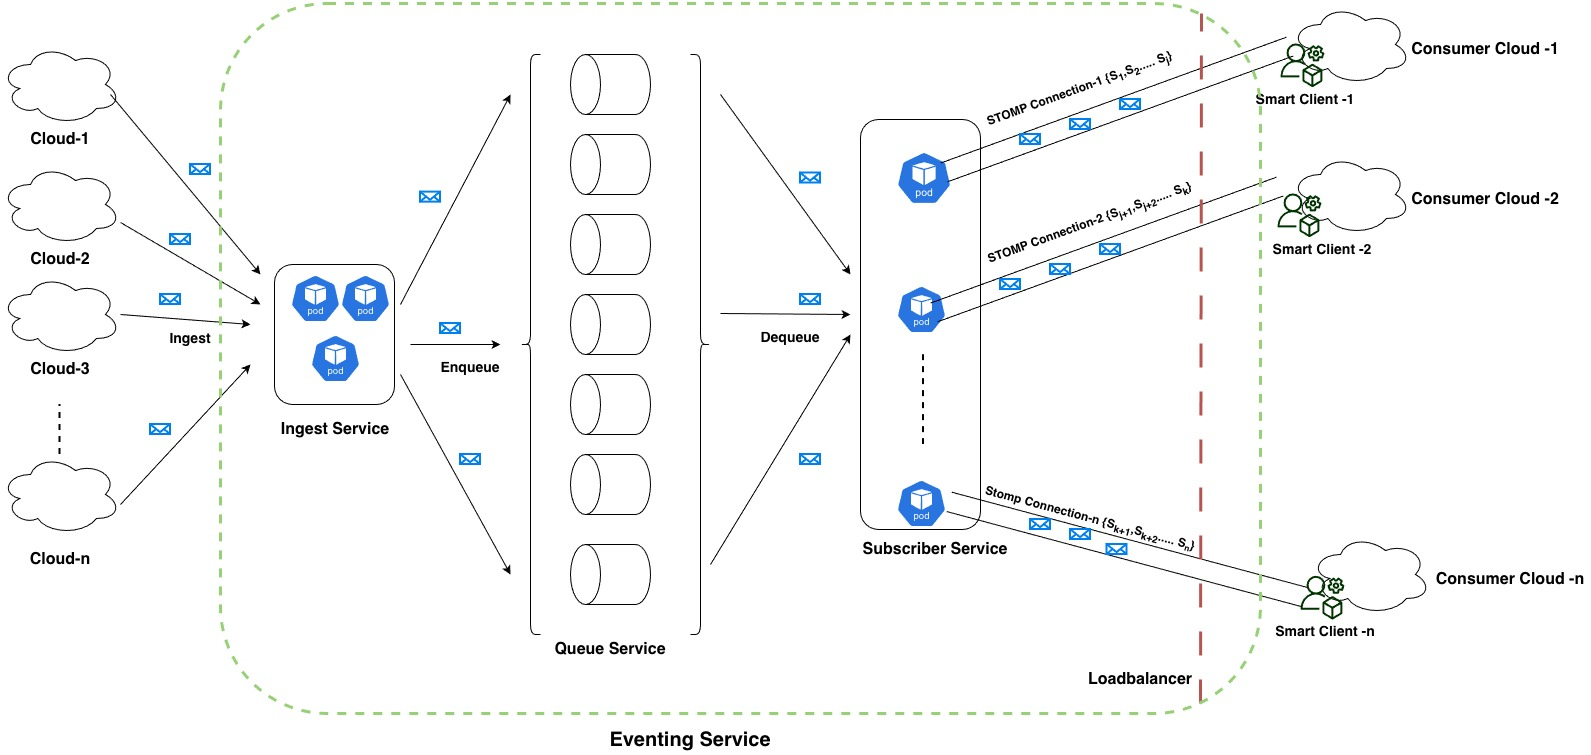
\includegraphics[width=\textwidth]{System-Architecture.jpg}
	\caption{System architecture with the DQL policy option shown. Producers send events through ingest services to durable subscription queues. Subscriber Pods deliver events over persistent connections. A client retains a load-balancer-assigned probe and promotes that same socket only after policy selection and execution checks. Greedy selection uses the same observation and actuation interfaces.}
	\Description{Left-to-right architecture diagram. Producer clouds send events through ingest pods into durable queues. Subscriber pods read those queues and accept persistent connections through a transport load balancer. On the right, a smart client maintains active connections, a subscription-free random probe, local queue metrics, a DQL controller, and a guarded action executor. Feedback arrows carry pod statistics to the client and connection operations back to the subscriber pods.}
	\label{fig:system_architecture}
\end{figure*}

\begin{landscape}
\begin{figure}[p]
	\centering
	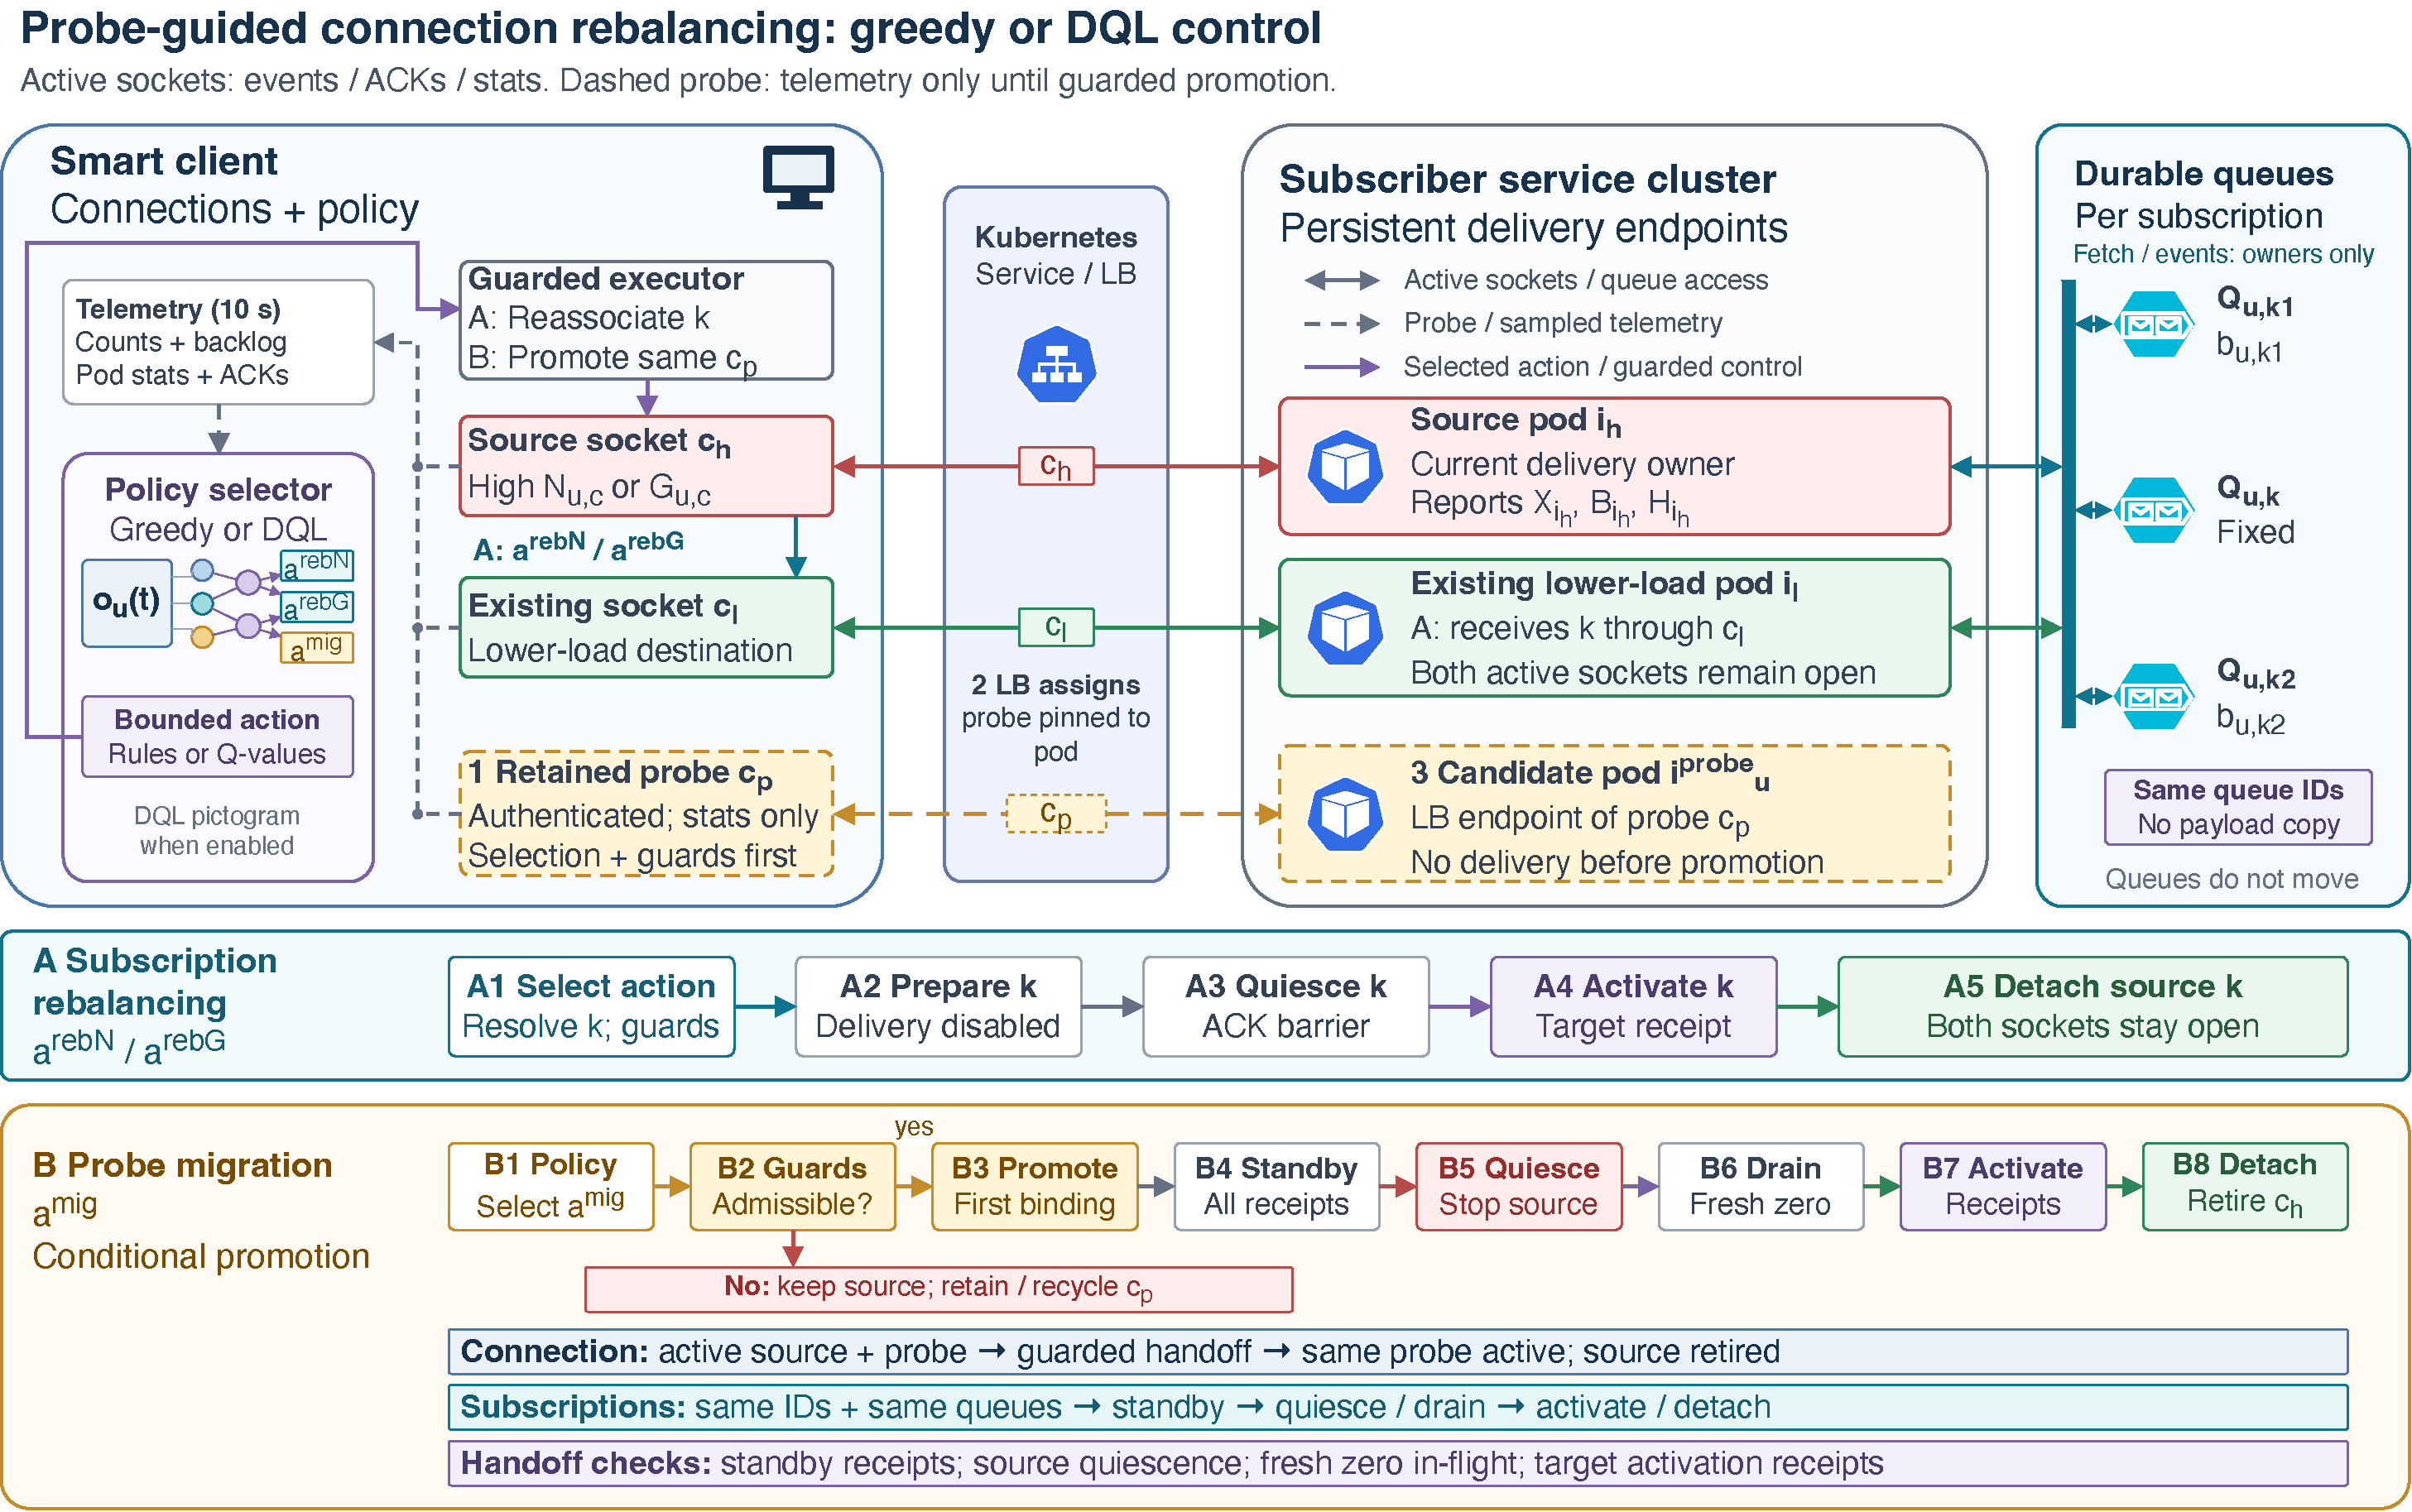
\includegraphics[width=\linewidth,height=0.83\textwidth,keepaspectratio]{figures/control-architecture-original-style.pdf}
	\caption{Shared probe-guided architecture with greedy or DQL selection. Path A rebalances subscriptions between existing sockets. Path B promotes the retained probe through its first standby binding, waits for all standby receipts, quiesces and drains the source, activates the target, detaches the source bindings, and retires the old socket. Unselected sockets and durable queues remain in place. The DQL pictogram denotes the optional learned selector, not an additional handoff service.}
	\Description{Two-path architecture with clients, subscriber Pods, and durable queues. Active and probe telemetry feed a greedy or DQL selector and a shared guarded executor. The selected probe keeps its load-balanced endpoint. Standby receipts, source quiescence, fresh zero-in-flight telemetry, activation receipts, and source detachment govern handoff. No ownership registry or epoch-commit service is shown.}
	\label{fig:control_architecture}
\end{figure}
\end{landscape}
\subsection{Event Producers and Ingest Service}

Event producers run in independent cloud environments, shown as Cloud-1 through Cloud-n in Figure~\ref{fig:system_architecture}. They generate events asynchronously and send them to the ingest service, which is the system's entry point.
The ingest service is implemented as a horizontally scalable set of service instances deployed as pods. Each ingest instance processes incoming events and enqueues them into the distributed queue service. The ingest service ensures reliable message intake and provides elasticity to handle fluctuating workloads.

\subsection{Queue Service}

The queue service acts as an intermediate buffering layer between event producers and subscribers. It provides durable storage and ensures reliable delivery of messages. Messages received from the ingest service are placed into queues, where they remain until consumed by subscriber services.The queue service supports parallel queues and can scale as event volume grows. Buffering lets producers and consumers work independently, without matching their processing rates.

\subsection{Subscriber Service}

The subscriber service is responsible for dequeuing messages from the queue service and delivering them to consumer clients. Similar to the ingest service, the subscriber service is deployed as multiple horizontally scalable instances.
Each subscriber service instance maintains persistent transport connections with multiple consumer clients. These connections may use STOMP-over-TCP, raw TCP, WebSocket, or another long-lived subscription-bearing transport. They allow real-time event delivery and enable clients to subscribe to specific event streams.
Subscriber service instances perform the following key functions:

\begin{itemize}
	\item Dequeue messages from the queue service
	\item Maintain subscription state for connected clients
	\item Deliver messages to subscribed clients
	\item Track subscription load, backlog, and delivery rate
\end{itemize}

The subscriber service instances are deployed behind a load balancer, which distributes incoming client connection requests across available subscriber instances.

\subsection{Load Balancer}

The load balancer serves as the initial connection routing layer between consumer clients and subscriber service instances. It distributes client connections across available subscriber instances using traditional transport-level algorithms such as round-robin or least-connections.

However, the load balancer operates without visibility into application-level metrics such as subscription count, message backlog, or processing load. As a result, connection assignments may not reflect the true load distribution across subscriber instances.
This limitation motivates the need for adaptive client-driven connection placement mechanisms.

\subsection{Consumer Clients and Persistent Transport Connections}

Consumer clients, referred to as Smart Clients in Figure~\ref{fig:system_architecture}, are deployed across multiple consumer cloud environments. These clients establish persistent subscription transport connections to subscriber service instances.

Each persistent transport connection can support multiple subscriptions. For
client $u$, let $\mathcal{K}_u(t)$ be its subscription set and
$\mathcal{C}_u(t)$ its active delivery-connection set. The subscriptions
assigned to connection $c\in\mathcal{C}_u(t)$ are

\begin{equation}
	\mathcal{K}_{u,c}(t)=\{k\in\mathcal{K}_u(t):z_{u,k,c}(t)=1\}.
\end{equation}

Here $z_{u,k,c}(t)$ is the binary assignment indicator defined in
Section~\ref{sec:problem-formulation}. Each subscription corresponds to a
specific event stream or topic; $k$ indexes a subscription, not a Pod.

The subscriber service maintains subscription state and delivers messages to clients based on these subscriptions.
Because subscription counts and event rates may vary significantly across connections, the load imposed by each client connection is highly variable.

\subsection{Connection Placement and Rebalancing Model}

Let the set of subscriber service instances be denoted as:

\begin{equation}
	\mathcal{S}=\{1,2,\ldots,n\}.
\end{equation}

Each subscriber instance exposes the following dynamic statistics to active
connections and probe connections:

\begin{equation}
	y_i(t)=\bigl(p_i,X_i(t),B_i(t),H_i\bigr).
\end{equation}

where:

\begin{itemize}
	\item $p_i$ is the pod name
	\item $X_i(t)$ is the pod-level subscription count
	\item $B_i(t)$ is the cumulative backlog over all subscription queues served by the pod
	\item $H_i$ is the configured maximum processing threshold, used only as a capacity-normalization signal
\end{itemize}

These statistics are exposed to clients through protocol-specific statistics
frames, headers, or control messages. Actual drain behavior is measured from the client side using delivered,
processed, and acknowledged message counts, because the effective drain rate also depends on client processing capacity.

Decentralized monitoring research similarly treats telemetry quality and
monitoring overhead as coupled concerns. DEMon, for example, uses adaptive
gossip-based monitoring in volatile edge environments \cite{Ilager2026DEMon}.
Here the telemetry scope is deliberately smaller: active sockets and a retained
probe provide sampled Pod observations, not a complete cluster view.

Clients maintain persistent connections and periodically evaluate alternative subscriber instances using a learning-based placement and rebalancing strategy. Based on observed load characteristics, clients may rebalance subscriptions across their own connections, scale connection parallelism, or migrate subscriptions to alternative subscriber instances.This adaptive mechanism enables the system to dynamically rebalance load across client connections and subscriber service instances while operating only on client-visible statistics.

\subsection{Retained-Probe Acquisition and Receipt-Gated Handoff}
\label{sec:probe_handoff}

Figure~\ref{fig:control_architecture} makes the selected-Pod mechanism
explicit. The client does not choose a Pod name and then attempt to bypass the
Kubernetes Service. It opens an authenticated, statistics-only probe through
the same transport load balancer used by ordinary connections. The load
balancer selects one ready subscriber Pod when that TCP/WebSocket connection is
established, after which the socket remains endpoint-bound to that Pod. The
STOMP implementation identifies the authenticated session and its Pod in
telemetry. A probe initially has no subscription bindings and does not fetch
events. Promotion changes the role of that existing session; it does not
create a second connection whose load-balanced destination might differ.

The selector evaluates a candidate that is already connected. Fresh and
sufficiently complete telemetry, a distinct source and target Pod, capacity,
cooldown, and handoff checks determine whether migration is admissible. The
DQL selector also applies its action-value hysteresis test. A rejected or
unselected probe remains statistics-only until refreshed or recycled. Thus,
probing does not imply migration, and the client never moves an established
TCP socket between endpoints. It replaces one delivery socket with the
already-connected probe and reassociates the source subscriptions.
In Figure~\ref{fig:control_architecture}, $c_p$ labels the retained probe,
whose endpoint is $i_u^{\mathrm{probe}}(t)$. The source and existing target Pod indices
are $i_h=i_{u,c_h}(t)$ and $i_l=i_{u,c_l}(t)$. Thus $i_h$ and $i_l$ identify
Pods, while $P_i(t)$ denotes a pressure score.

Queued events remain in the same durable subscription queues $Q_{u,k}(t)$.
The client retains each subscription identifier, listener, message permits,
and negative-acknowledgement visibility setting. For the selected subscription
set $\mathcal{K}_{\mathrm{move}}$, the executed protocol is:
\begin{enumerate}
	\item Create each target binding in \emph{standby}, waiting for its STOMP
	receipt. The first subscription request carries the probe-promotion flag.
	The server checks the authenticated session and its active-connection cap,
	then changes the probe's role. Standby bindings do not deliver events.
	The source remains active while these target bindings are prepared.
	\item After all standby receipts, add the promoted socket to the client
	pool and clear its probe role. Send a receipt-gated quiesce request for each
	source binding. Quiescence stops new delivery while existing in-flight
	messages remain on the source acknowledgement path.
	\item Record a barrier timestamp after the quiesce requests. Wait for a
	newer source telemetry frame that reports every selected subscription as
	quiesced with zero in-flight messages. A zero from an older frame cannot
	satisfy the barrier. Drain time is observed, not estimated from $H_i$.
	\item Activate the target bindings one at a time, waiting for their
	receipts. The source remains quiesced during this phase.
	\item Unsubscribe the source bindings with receipt checks. After all
	selected bindings are detached, remove and disconnect the old socket for
	a full-connection migration. Replenish the subscription-free probe
	asynchronously. Unselected active sockets remain connected.
\end{enumerate}

Let $s_b$ be the barrier timestamp, $s_f$ the timestamp of a received source
frame, and $I_{c_h,k}(s_f)$ its reported in-flight count. The target-activation
precondition is
\begin{equation}
	 s_f\geq s_b\quad\land\quad
	 \bigwedge_{k\in\mathcal{K}_{\mathrm{move}}}
	 \left[\operatorname{state}_{c_h,k}(s_f)=\mathrm{quiesced}
	 \land I_{c_h,k}(s_f)=0\right].
	\label{eq:handoff_barrier}
\end{equation}
This precondition describes the implemented planned handoff, assuming timely,
accurate telemetry and servers that honor quiescence. It is not a distributed
ownership lease or an epoch-fencing guarantee during partitions. On an
exception, the client attempts to quiesce and close the target before restoring
the source; unsuccessful cleanup is logged rather than counted as a completed
handoff. The protocol uses authenticated session state and receipts, not a
separate signed promotion token or an atomic cross-Pod ownership commit.
Receipt completion records server acknowledgement of the corresponding
operation; it is not by itself proof of an end-to-end exactly-once event census.
The delivery model remains unordered and permits redelivery after an
unconfirmed acknowledgement. The live results report observed deliveries,
ACK receipts, and unresolved records separately.

\subsection{System Characteristics}

The system exhibits the following important properties:

\begin{itemize}
	
	\item \textbf{Persistent connections.} Clients maintain long-lived STOMP-over-TCP,
	raw TCP, WebSocket, or equivalent subscription-bearing connections.
	
	\item \textbf{Subscription-Based Load:} Server load is determined primarily by subscription count and event rate, rather than connection count.
	
	\item \textbf{Dynamic Workload:} Event rates and subscription distributions change over time.
	
	\item \textbf{Distributed Architecture:} Subscriber services operate independently and scale horizontally.
	
	\item \textbf{Limited Load Balancer Visibility:} Load balancers lack application-level visibility into subscription load.
	
\end{itemize}

These characteristics make adaptive, client-driven connection placement particularly suitable for achieving optimal load balancing.




\section{Problem Formulation}
\label{sec:problem-formulation}

The main quantities are client subscriptions $\mathcal{K}_u$, active sockets
$\mathcal{C}_u$, per-subscription backlog $b_{u,k}$, and the corresponding
connection loads $(N_{u,c},G_{u,c})$. Pod-wide quantities $(X_i,B_i)$ include
all clients served by Pod $i$. Appendix~\ref{app:notation} collects the full
symbol reference; definitions also appear at their first use below.

We model the system at discrete control epochs $t=0,1,\ldots,T$. The interval
between adjacent epochs is $\Delta$ seconds: the next epoch is $t+1$, while
its physical time is $(t+1)\Delta$. Live-event timestamps and durations are
reported separately in seconds. Let
$\mathcal{S}=\{1,\ldots,n\}$ be the set of subscriber pods and
$\mathcal{U}=\{1,\ldots,m\}$ be the set of clients. Client $u$ maintains a
subscription set $\mathcal{K}_u(t)$ and a set of persistent transport
connections $\mathcal{C}_u(t)$, with
$1\leq |\mathcal{C}_u(t)|\leq C_{\max}$.
Indices $i,u,c,k$ refer to Pods, clients, connections, and subscriptions,
respectively. Calligraphic symbols denote sets; their cardinalities are
counts. In the single-client scaling rules, $C(t)=|\mathcal{C}_u(t)|$ and
$N_{\mathrm{sub}}(t)=|\mathcal{K}_u(t)|$ are count shorthands with the fixed client
index suppressed. They are never used as sets. Figure labels and algorithm
steps may omit $(t)$ when all quantities refer to the same decision epoch.

\subsection{Per-Subscription Queues}

Each subscription has a queue that stores messages waiting to be delivered and
processed. Let $Q_{u,k}(t)$ be the queue of subscription
$k\in\mathcal{K}_u(t)$, and let
\begin{equation}
	b_{u,k}(t)=|Q_{u,k}(t)|
\end{equation}
be the backlog for that subscription. This is the basic backlog measure used
by the client. At the pod level, backlog is a
server-owned aggregate. Let $\mathcal{R}_i(t)$ denote the set of subscription
queues currently served by pod $i$, and let $\tilde{b}_{i,r}(t)$ be the backlog
of server-side subscription queue $r\in\mathcal{R}_i(t)$. If queue $r$
corresponds to client $u$ and subscription $k$, then $\tilde{b}_{i,r}(t)$ is
the server-side counterpart of $b_{u,k}(t)$; however, $\mathcal{R}_i(t)$ also
contains queues belonging to other clients and is maintained by the pod, not by
any single client.

Let $z_{u,k,c}(t)\in\{0,1\}$ indicate whether subscription $k$ of client $u$ is
assigned to connection $c\in\mathcal{C}_u(t)$. Feasible assignment requires
\begin{equation}
	\sum_{c\in\mathcal{C}_u(t)} z_{u,k,c}(t)=1,
	\qquad \forall u,\; k\in\mathcal{K}_u(t).
	\label{eq:subscription_assignment}
\end{equation}
Let $i_{u,c}(t)\in\mathcal{S}$ denote the pod index reached by connection
$c$. This endpoint mapping differs from the Pod name $p_i$ and from the
selected DQL action $a_u(t)$.
The number of subscriptions and cumulative subscription backlog on connection
$c$ are
\begin{align}
	N_{u,c}(t) &= \sum_{k\in\mathcal{K}_u(t)} z_{u,k,c}(t),\\
	G_{u,c}(t) &= \sum_{k\in\mathcal{K}_u(t)}
	b_{u,k}(t)z_{u,k,c}(t).
	\label{eq:connection_backlog}
\end{align}
The first term captures subscription-management pressure on the connection; the
second captures queue pressure induced by the subscriptions mapped to that
connection.

\subsection{Pod Statistics and Partial Observability}

Each pod exposes a statistics tuple through active connections and probe
connections:
\begin{equation}
	y_i(t)=\bigl(p_i,\; X_i(t),\; B_i(t),\; H_i\bigr),
	\label{eq:pod_stats}
\end{equation}
Here $p_i$ is the pod name, and $X_i(t)$ is its subscription count.
The value $B_i(t)$ is the cumulative backlog across all subscription queues
served by pod $i$. The value $H_i$ is the configured maximum processing threshold. Using the
server-side queue set $\mathcal{R}_i(t)$, the pod-level subscription count and
cumulative pod backlog are
\begin{equation}
	X_i(t)=|\mathcal{R}_i(t)|,\qquad
	B_i(t)=
	\sum_{r\in\mathcal{R}_i(t)}
	\tilde{b}_{i,r}(t).
	\label{eq:pod_backlog}
\end{equation}
Thus $B_i(t)$ is not defined by summing over the connection set
$\mathcal{C}_u(t)$ of a particular client. A client's connections determine
which pod statistics it can observe and which subscriptions it can move, but
the pod backlog itself is the cumulative backlog over all subscription queues
served by that pod. These pod-level values include traffic from many clients
and are not directly computable by a single client unless reported by the pod.

At each statistics interval $\Delta$ (10 seconds in the target deployment),
every active connection receives the tuple of its current pod. In addition,
client $u$ maintains one authenticated probe connection whose endpoint is
selected by the load balancer and receives its tuple. The client
retains the probe socket and its endpoint identity until promotion, expiry, or
recycling; it does not resample a different pod merely by reading the next
observation. Therefore the client observes only a subset
$\mathcal{O}_u(t)\subseteq\mathcal{S}$ of pod states:
\begin{equation}
	\mathcal{O}_u(t)=
	\{i_{u,c}(t):c\in\mathcal{C}_u(t)\}
	\cup
	\{i^{\mathrm{probe}}_u(t)\}.
\end{equation}
The client stores the newest tuple for each observed pod in a local cache. This
makes the placement problem partially observable: global cluster variance is
available to an offline evaluator or simulator, but not to an individual client
controller. In particular, an admissible migration target must be represented
by a currently retained probe socket; the client cannot replace the sampled
candidate with an unobserved globally optimal pod.

\begin{assumption}[Available deployment signals]
For every pod $i$ observed by client $u$, where $i\in\mathcal{O}_u(t)$, the
protocol supplies $(p_i,X_i(t),B_i(t),H_i)$ in a statistics frame, header, or
control message. Client
$u$ can also measure its own per-subscription backlogs $b_{u,k}(t)$, delivered
message count, processed message count, acknowledged message count, active
connection count, and migration count over each interval $\Delta$.
\end{assumption}

\begin{assumption}[Transport abstraction]
The underlying transport is required only to maintain long-lived client--pod
connections, multiplex one or more subscriptions over a connection, support
subscription migration or reassignment, and expose periodic statistics through
headers, frames, or control messages. STOMP-over-TCP, custom TCP streams, and
WebSocket-based messaging are concrete examples of this abstraction.
\end{assumption}

\begin{remark}
The pod threshold $H_i$ is not treated as an actual drain rate. The true drain
rate depends on the queue subsystem, pod scheduling, network transport,
connection behavior, client processing capacity, and acknowledgement rate.
Hence $B_i(t)/(H_i\Delta+\varepsilon_0)$ is used only as a dimensionless
pod-side pressure ratio. Here $B_i$ counts messages, $H_i$ has units of
events per second, and $\varepsilon_0$ has units of messages. The ratio is
not an estimate of the actual drain time.
\end{remark}

\subsection{Local Imbalance Measures}

For client $u$, define the mean subscription count and mean backlog load across
its own connections:
\begin{align}
	\bar{N}_u(t)
	&= \frac{1}{|\mathcal{C}_u(t)|}
	\sum_{c\in\mathcal{C}_u(t)} N_{u,c}(t),\\
	\bar{G}_u(t)
	&= \frac{1}{|\mathcal{C}_u(t)|}
	\sum_{c\in\mathcal{C}_u(t)} G_{u,c}(t).
\end{align}
The corresponding variances are
\begin{align}
	V^N_u(t)
	&= \frac{1}{|\mathcal{C}_u(t)|}
	\sum_{c\in\mathcal{C}_u(t)}
	\bigl(N_{u,c}(t)-\bar{N}_u(t)\bigr)^2,\\
	V^G_u(t)
	&= \frac{1}{|\mathcal{C}_u(t)|}
	\sum_{c\in\mathcal{C}_u(t)}
	\bigl(G_{u,c}(t)-\bar{G}_u(t)\bigr)^2.
\end{align}
The first variance captures subscription-management skew, while the second
captures backlog skew. The local rebalancing objective is therefore
\begin{equation}
	V_u(t)=
	\eta_N\widehat{V}^N_u(t)
	+\eta_G\widehat{V}^G_u(t),
	\qquad
	\eta_N+\eta_G=1,
	\label{eq:local_connection_imbalance}
\end{equation}
where hats denote normalized quantities. This formulation is necessary because
two connections can have equal backlog but very different subscription counts,
or equal subscription counts but very different backlog.
The normalized terms place the two variances on a common scale before they are
combined. In the evaluation setup, we use positive reference values
$V^N_{\mathrm{ref}}$ and $V^G_{\mathrm{ref}}$ and compute
\begin{align*}
	\widehat{V}^N_u(t)
	&=\min\left\{\frac{V^N_u(t)}{V^N_{\mathrm{ref}}},1\right\},\\
	\widehat{V}^G_u(t)
	&=\min\left\{\frac{V^G_u(t)}{V^G_{\mathrm{ref}}},1\right\}.
\end{align*}
Thus $V_u(t)$ is a dimensionless connection-imbalance score in which the
subscription-count component and the backlog-load component are comparable.
The subscription-count reference $V^N_{\mathrm{ref}}$ is chosen from an
operational tolerance rather than learned by DQL. Since
$\sqrt{V^N_u(t)}$ is the standard deviation of subscription counts across
client $u$'s active connections, a tolerable subscription-count standard
deviation $\sigma^{N}_{\mathrm{tol}}$ defines
\[
	V^N_{\mathrm{ref}}=(\sigma^{N}_{\mathrm{tol}})^2.
\]
For example, if the operator allows roughly a $\Delta_N$-subscription spread
between a heavy and a light connection, then
$\sigma^{N}_{\mathrm{tol}}\approx \Delta_N/2$ is a practical calibration. If
the subscription-density threshold is $\Theta_N$, a default choice is
$\sigma^{N}_{\mathrm{tol}}=\rho_N\Theta_N$ with
$\rho_N\in[0.1,0.25]$; smaller values increase sensitivity to
subscription-count skew.
The backlog-load reference $V^G_{\mathrm{ref}}$ is chosen in the same way,
but in backlog units. Since $\sqrt{V^G_u(t)}$ is the standard deviation of
cumulative connection backlog $G_{u,c}(t)$ across client $u$'s active
connections, a tolerable backlog-load standard deviation
$\sigma^{G}_{\mathrm{tol}}$ defines
\[
	V^G_{\mathrm{ref}}=(\sigma^{G}_{\mathrm{tol}})^2.
\]
If the operator allows roughly a $\Delta_G$-message backlog spread between a
heavy and a light connection, then
$\sigma^{G}_{\mathrm{tol}}\approx \Delta_G/2$ is the direct calibration. When
the tolerance is latency-driven, $\Delta_G$ is derived from the
client-observed processing capability rather than from pod capacity alone. For
example, if $\widehat{r}^{\mathrm{ack}}_{u}$ is a conservative ACK or processing rate
measured by client $u$ and $\tau_G$ is the acceptable additional drain-time
skew, then $\Delta_G=\widehat{r}^{\mathrm{ack}}_{u}\tau_G$ is a defensible choice. If
no latency SLO is available, a practical default is
$\sigma^{G}_{\mathrm{tol}}=\rho_G\beta\Theta_N$ with
$\rho_G\in[0.1,0.25]$, where $\beta\Theta_N$ is the nominal backlog budget of
a connection carrying $\Theta_N$ subscriptions.
The weights $\eta_N,\eta_G\geq0$ determine how much the controller prioritizes
subscription-management fairness versus backlog-load fairness. For example,
larger $\eta_N$ makes the controller more sensitive to connections carrying
too many subscriptions, while larger $\eta_G$ makes it more sensitive to
connections accumulating more queued messages. The constraint
$\eta_N+\eta_G=1$ makes $V_u(t)$ a convex combination rather than an
unbounded sum.

\subsection{Pod Pressure and Deployable Reward}

For an observed pod $i\in\mathcal{O}_u(t)$, define normalized pressure terms
\begin{align}
	P^X_i(t) &= \min\left\{\frac{X_i(t)}{X_{\mathrm{safe}}},1\right\},\\
	P^B_i(t) &= \min\left\{\frac{B_i(t)}{B_{\mathrm{ref}}},1\right\},\\
	P^H_i(t) &= \min\left\{\frac{B_i(t)}{H_i\Delta+\varepsilon_0},1\right\},
	\qquad \varepsilon_0>0.
\end{align}
Here $X_{\mathrm{safe}}$ is the subscription count at which pod reliability begins to
degrade. The value $X_{\mathrm{hard}}$ is the hard reference count at which we treat the
pod as severely overloaded by subscription-management work.
The value $B_{\mathrm{ref}}$ is the backlog reference used for normalization. The condition
$X_{\mathrm{hard}}>X_{\mathrm{safe}}$ is required. Since high subscription count has been
observed to make connections unreliable, we also define a nonlinear
reliability-risk penalty
\begin{equation}
	P^R_i(t)=
	\left[
	\frac{X_i(t)-X_{\mathrm{safe}}}
	{X_{\mathrm{hard}}-X_{\mathrm{safe}}}
	\right]_+^2,
	\qquad [x]_+=\max\{x,0\}.
\end{equation}
The pod pressure score is
\begin{align}
	P_i(t)=
	&\omega_X P^X_i(t)
	+\omega_B P^B_i(t) \nonumber\\
	&+\omega_H P^H_i(t)
	+\omega_R P^R_i(t),
	\label{eq:pod_pressure}\\
	&\sum_{q\in\{X,B,H,R\}}\omega_q=1,\qquad \omega_q\geq 0. \nonumber
\end{align}
Here $P^X_i(t)$ measures normalized subscription-count pressure.
The term $P^B_i(t)$ measures normalized cumulative-backlog pressure.
The term $P^H_i(t)$ measures backlog pressure relative to the processing threshold.
Finally, $P^R_i(t)$ measures nonlinear reliability risk and becomes active only
when $X_i(t)>X_{\mathrm{safe}}$. The coefficients
$\omega_X,\omega_B,\omega_H,\omega_R$ specify how much importance the policy
assigns to each pressure component. For example, if subscription-heavy pods are
known to become unreliable before backlog becomes large, then $\omega_X$ and
$\omega_R$ receive greater weight than $\omega_B$ and $\omega_H$. If queue
accumulation is the dominant failure mode, $\omega_B$ and $\omega_H$
receive greater weight. This score keeps subscription count and backlog
count as distinct load dimensions.

Client $u$ also computes local backlog and backlog-growth pressure:
\begin{align}
	B_u(t) &= \sum_{k\in\mathcal{K}_u(t)} b_{u,k}(t),\\
	\mathrm{Grow}_u(t) &= \bigl[B_u(t)-B_u(t-1)\bigr]_+,\qquad t\geq1.
\end{align}
At initialization, $\mathrm{Grow}_u(0)=0$. Let $T_u(t)$ be the effective client-side
throughput in events per second. The rates $T^{\mathrm{del}}_u(t)$, $T^{\mathrm{proc}}_u(t)$,
and $T^{\mathrm{ack}}_u(t)$ are the delivered, processed, and acknowledged counts in
the measured interval, each divided by its duration $\Delta$:
\begin{equation}
	T_u(t)=
	\min\{T^{\mathrm{del}}_u(t),T^{\mathrm{proc}}_u(t),T^{\mathrm{ack}}_u(t)\}.
\end{equation}
For an action that selects or keeps pod $i$, the deployable reward is
\begin{align}
	R_u(t)=
	&-\lambda_1\widehat{B}_u(t)
	-\lambda_2\widehat{\mathrm{Grow}}_u(t)
	-\lambda_3 P_i(t)
	-\lambda_4 V_u(t) \nonumber\\
	&-\lambda_5 M_u(t)
	-\lambda_6\widehat{C}_u(t)
	+\lambda_7\widehat{T}_u(t),
	\label{eq:deployable_reward}
\end{align}
where $M_u(t)$ is the migration indicator or normalized migration count,
$\widehat{C}_u(t)=|\mathcal{C}_u(t)|/C_{\max}$, and
$\lambda_\ell\geq0$ with $\sum_{\ell=1}^{7}\lambda_\ell=1$.
The hats on backlog, backlog growth, and throughput denote their normalized
versions under the stated experiment's scaling convention, not different
physical quantities. This reward is computable by the client from
local measurements and observed pod tuples.

\subsection{DQL State, Action, and Value Function}

The client-side controller is modeled as a partially observable sequential
decision problem. At each control epoch, client $u$ constructs an observation
vector
\begin{equation}
	o_u(t)=
	\left[
	o^B_u(t),o^N_u(t),o^G_u(t),o^C_u(t),o^P_u(t),o^D_u(t)
	\right],
	\label{eq:dql_observation}
\end{equation}
where $o^B_u(t)$ contains normalized local backlog and backlog growth.
The branch $o^N_u(t)$ describes subscription-count imbalance using terms such as
$N_{u,c}(t)$ and $V^N_u(t)$. The branch $o^G_u(t)$ describes backlog imbalance
using terms such as $G_{u,c}(t)$ and $V^G_u(t)$.
The branch $o^C_u(t)$ contains connection count and effective throughput.
The branch $o^P_u(t)$ contains pressure, subscription count, and cumulative
backlog for the current and probe pods. Finally, $o^D_u(t)$ contains cooldown
and statistics-staleness features. For current-pod features, $c^\star$ denotes
the connection being evaluated. All quantities are normalized before they
enter the Q-network.

The DQL action space is defined using bounded action templates rather than all
possible subscription assignments, which keeps the decision problem tractable:
\begin{equation}
	\mathcal{A}=
	\{a^{\mathrm{stay}},a^{\mathrm{reb}N},a^{\mathrm{reb}G},a^{\mathrm{scale}+},a^{\mathrm{scale}-},a^{\mathrm{mig}}\}.
	\label{eq:dql_actions}
\end{equation}
Here $a^{\mathrm{stay}}$ makes no change. The action $a^{\mathrm{reb}N}$ moves one subscription
from the connection with the most subscriptions to the one with the fewest.
The action $a^{\mathrm{reb}G}$ moves the subscription with the largest predicted decrease
in backlog variance. The action $a^{\mathrm{scale}+}$ opens one new connection and,
when allowed, makes bounded subscription moves toward the target $\Theta_N$.
The action $a^{\mathrm{scale}-}$ closes a subscription-free connection only if the
remaining connections meet the required capacity and observed backlog is zero.
The action $a^{\mathrm{mig}}$ requests promotion of the retained probe. It transfers the
evaluated connection or bounded subscription group only if the admissibility
and hysteresis conditions pass. The DQL network selects
the action template; it does not choose an arbitrary Pod or directly change a
subscription assignment. The deterministic executor computes the concrete
source connection, target connection, and subscription using the load-aware
rules in Algorithms~\ref{alg:adaptive_parallel_scaling} and
\ref{alg:connection_rebalancing}, and may reject an inapplicable template as a
guarded no-op.

The scale-up action is one logical option even though its guarded executor can
contain several reassociations. After the new socket is ready, the executor
repeatedly applies the same receipt-gated $a^{\mathrm{reb}N}$ primitive while
$\max_c N_{u,c}(t)>\Theta_N$ and an eligible move exists. It records the opened
session, completed move count, final maximum count, elapsed time, and whether
the target was restored. If opening fails, the unused socket is removed. If a
later reassociation fails, the completed receipt-gated moves remain valid and
the option reports failure rather than claiming an atomic rollback of the
whole sequence. New checkpoints carry an action-contract version.
Full-action execution rejects the older open-only meaning of
$a^{\mathrm{scale}+}$. An explicit rebalancing-only allowlist may load a legacy
checkpoint because it disables both scaling actions. This is the profile used
in the October loaded cluster trial. Table~\ref{tab:action-contract-map}
separates the evaluated contracts; the legacy checkpoint is not evidence for
learned cap-restoring scale-up.

DQL uses two action-value networks with the same architecture but different
roles. The online network $Q_\theta(o,a)$ is the trainable network used for
current action evaluation and epsilon-greedy action selection. The target
network $Q_{\theta^-}(o,a)$ is a delayed copy of the online network. It is not
used for selecting the live action and is not updated by every gradient step;
it is used only to compute a stable Bellman target for the next observation.
For a transition
$\xi_t=(o_u(t),a_u(t),R_u(t),o_u(t+1))$ sampled from replay buffer
$\mathcal{D}$, the target is
\begin{equation}
	y_t =
	R_u(t) + \gamma
	\max_{a'\in\mathcal{A}^{\mathrm{adm}}_u(t+1)}Q_{\theta^-}(o_u(t+1),a'),
	\label{eq:dql_target}
\end{equation}
where $\gamma\in[0,1)$ is the discount factor and $\theta^-$ denotes the target
network parameters. The set $\mathcal{A}^{\mathrm{adm}}_u(t+1)\subseteq\mathcal{A}$
contains the actions admitted by the next observation's execution guards;
an infeasible action cannot supply the bootstrap value. The equation applies
to non-terminal transitions. At a true terminal state, $y_t=R_u(t)$.
An interrupted observation window is not assigned an artificial terminal
reward. The online network parameters $\theta$ are trained by
minimizing
\begin{equation}
	\mathcal{L}(\theta)=
	\mathbb{E}_{\xi_t\sim\mathcal{D}}
	\left[
	\left(y_t-Q_\theta(o_u(t),a_u(t))\right)^2
	\right].
	\label{eq:dql_loss}
\end{equation}
Every $K_{\mathrm{sync}}$ training updates, the target network is synchronized by copying the
online parameters, $\theta^- \leftarrow \theta$. This separation prevents the
same rapidly changing network from defining both the prediction
$Q_\theta(o_u(t),a_u(t))$ and the target $y_t$. The parameters $\theta$ and
$\theta^-$ contain all network weights and biases; $\Theta_N$ is instead a
subscription-count threshold. The learning rate $\alpha$ controls the update
$\theta\leftarrow\theta-\alpha\nabla_\theta\mathcal{L}(\theta)$ and is
distinct from the imbalance weights $\eta_N,\eta_G$.
This formulation makes rebalancing a sequential control problem: a migration,
new connection, or subscription move can reduce future backlog but may incur
immediate migration or connection cost.

\subsubsection{Persistent Learning and Frozen Evaluation}
Learning is retained between runs through two checkpoint types. A research
checkpoint stores both networks' weights and biases, replay transitions and
their next-state action masks, the random-generator state, the exploration
rate, the training-update count, and the learner configuration. Restoring this
checkpoint continues the learner from its saved state rather than initializing
new weights. Simulator continuation starts fresh workload episodes; the
checkpoint does not restore an interrupted Kubernetes deployment or simulator
trajectory. Checkpoints also retain the action-contract version so that replay
from incompatible action meanings is not silently combined.

Each eligible transition is recorded before its model update, using the
action actually applied and the subsequent observed reward. A masked decision
or shadow recommendation is not evidence that a migration occurred; shadow
execution contributes only its applied stay action. Stale or incomplete
telemetry interrupts the learning trajectory instead of joining observations
across the missing interval. An append-only transition record and checkpoint
hashes preserve a traceable history of later training.

A deployment checkpoint is a separate frozen copy: exploration is disabled,
network updates are disabled, and replay is not modified during evaluation.
The evaluation records observations and outcomes without turning them into
training data for that comparison. Further development uses separately
designated training data and produces a new candidate, which requires its own
validation before deployment. Thus, retained learning avoids restarting from
zero without making a fixed-policy experiment adapt to its test outcomes.

\subsection{Global Evaluation Objective}

The controller does not require cluster-wide variance. However, simulation and
offline validation can report global metrics. A finite-horizon evaluation cost
is
\begin{align}
	J_T =
	\sum_{t=0}^{T}
	\Bigl[
	&\Lambda_B \sum_{i\in\mathcal{S}}B_i(t)
	+\Lambda_X \Phi_X(t) \nonumber\\
	&+\Lambda_C \sum_{u\in\mathcal{U}}V_u(t)
	+\Lambda_M M(t)
	\Bigr].
\end{align}
where $\Phi_X(t)$ is pod subscription-count variance and $M(t)$ is total
migration count. This objective is used to evaluate system-level behavior, not
as information assumed available to every client.

The quantity $J_T$ is an offline finite-horizon cost: lower values indicate
better system-level behavior over the evaluation horizon $0,\ldots,T$. The
first term penalizes total pod backlog, where $B_i(t)$ is the cumulative
backlog over all subscription queues served by pod $i$. The second term
penalizes uneven subscription placement across pods. Specifically, if
\begin{align*}
	\bar{X}(t)
	&=\frac{1}{|\mathcal{S}|}\sum_{i\in\mathcal{S}}X_i(t),\\
	\Phi_X(t)
	&=\frac{1}{|\mathcal{S}|}
	\sum_{i\in\mathcal{S}}\bigl(X_i(t)-\bar{X}(t)\bigr)^2,
\end{align*}
then $\Phi_X(t)$ is high when some pods carry many more subscriptions than
others. The third term aggregates client-side connection imbalance, using
$V_u(t)$ from (\ref{eq:local_connection_imbalance}); it measures whether a
client's own persistent connections are uneven in subscription count or
backlog load. The fourth term penalizes operational churn through $M(t)$, the
number of migration or reconnect operations performed during epoch $t$.
The coefficients
$\Lambda_B,\Lambda_X,\Lambda_C,\Lambda_M\geq 0$ determine the relative
importance of backlog reduction, pod-level subscription balance, client-side
connection balance, and migration stability. Normalization before weighting
places the components on comparable scales, preventing a large-scale metric
from dominating $J_T$ merely because of its units.

\subsection{Rebalancing Properties}

\begin{proposition}[Subscription-density bound]
If $1\leq|\mathcal{K}_u(t)|\leq \Theta_N C_{\max}$ and the scaling rule sets
\begin{equation}
	|\mathcal{C}_u(t)| =
	\left\lceil\frac{|\mathcal{K}_u(t)|}{\Theta_N}\right\rceil,
\end{equation}
then the mean subscription density satisfies $\bar{N}_u(t)\leq\Theta_N$.
\end{proposition}

\begin{proof}
By definition, $\bar{N}_u(t)=|\mathcal{K}_u(t)|/|\mathcal{C}_u(t)|$. Since
$|\mathcal{C}_u(t)|\geq |\mathcal{K}_u(t)|/\Theta_N$, it follows that
$\bar{N}_u(t)\leq\Theta_N$.
\end{proof}

\begin{proposition}[Backlog-variance reduction]
For client $u$, let $c_h,c_l\in\mathcal{C}_u(t)$ be two active persistent
connections, where $c_h$ is the source connection from which subscription $k$
is removed and $c_l$ is the target connection to which subscription $k$ is
assigned. Let $G_{u,c_h}(t)$ and $G_{u,c_l}(t)$ be the cumulative backlog loads
on these two connections before the move, and let $b_{u,k}(t)>0$ be the backlog
of the moved subscription queue. If
\begin{equation}
	G_{u,c_h}(t)-G_{u,c_l}(t)>b_{u,k}(t),
\end{equation}
then moving subscription $k$ from $c_h$ to $c_l$ strictly decreases the
connection-level backlog variance $V^G_u(t)$.
\end{proposition}

The condition states that the source connection is heavier than the target
connection by more than the backlog carried by the moved subscription. Hence
the move reduces their squared-deviation sum. It can cross the equal-load
point and still reduce variance: loads $(10,0)$ become $(2,8)$ after a move
of size 8. Avoiding that crossing would require the stronger condition
$2b_{u,k}(t)\leq G_{u,c_h}(t)-G_{u,c_l}(t)$, which is not needed by the proposition.

\begin{proof}
The move preserves total backlog and therefore preserves $\bar{G}_u(t)$. Let
$d_h=G_{u,c_h}(t)-\bar{G}_u(t)$ and
$d_l=G_{u,c_l}(t)-\bar{G}_u(t)$. Only two squared-deviation terms change. With
$b=b_{u,k}(t)$, the unnormalized variance change is
\begin{align}
	&(d_h-b)^2+(d_l+b)^2-d_h^2-d_l^2 \nonumber\\
	&\quad =
	2b\bigl(b-(G_{u,c_h}(t)-G_{u,c_l}(t))\bigr)<0.
\end{align}
Thus $V^G_u(t)$ decreases.
\end{proof}

\begin{remark}
The placement loop optimizes a client-observed reward rather than an
unobserved global cluster objective. It is a decentralized control mechanism operating
under partial observability: active connections and probe connections provide
fresh but incomplete pod statistics, and the client optimizes its own reward
using these observations.
\end{remark}

\section{Policy Selection and Guarded Rebalancing}
The framework places a policy selector above three concrete runtime mechanisms:
pod migration, client-side connection scaling, and subscription redistribution
across active connections. These mechanisms solve different parts of the same
load-distribution problem. Migration changes where a connection terminates,
scaling changes how much parallelism the client maintains, and rebalancing
changes how subscriptions use that parallelism. Keeping the mechanisms
separate makes each action deployable, while the selected policy decides which
action is appropriate at a given control epoch.

The separation between reward and feasibility is deliberate. Safe-RL research
distinguishes performance optimization from constraint satisfaction
\cite{Gu2024SafeRL}; a migration penalty alone cannot enforce ownership or
readiness. Krasowski et al. distinguish action masking, replacement, and
projection as intervention mechanisms \cite{Krasowski2023ProvablySafe}.
Our masks and execution-time checks restrict the deployable actions, but do
not confer the formal safety guarantees of a verified environment model.

\subsection{Greedy and Learned Policy Roles}
Both policy families use the client-visible measurements and deterministic
execution checks defined above. In the scale-out study, the guarded-greedy
selector requests $a^{\mathrm{mig}}$ whenever that action is admissible and
otherwise stays. Its guard assesses projected source and target pressure
after moving the selected subscription group, so a lightly subscribed but
heavily backlogged candidate need not be accepted. The source-selection and
pressure checks are shared with DQL; they are not learned from DQL's outcomes.

The mixed-workload study uses a different deterministic comparator, labelled
\emph{Heuristic}: it applies threshold rules for subscription-count and backlog
imbalance as well as migration. The independent \emph{Scripted} timing controls
use pressure-unaware schedules and are sensitivity controls, not substitutes
for the stronger guarded-greedy comparison. Table~\ref{tab:policy-roles}
keeps these identities distinct.

\begin{table}[!htbp]
\centering\small
\caption{Policy roles and the comparison each supports. Greedy and DQL share
the rebalancing mechanism; the studies retain their original policy labels.}
\Description{Five policy rows distinguish pressure-aware greedy migration,
the multidimensional heuristic, DQL, random scripted schedules, and unchanged placement.}
\label{tab:policy-roles}
\begin{tabular}{p{0.19\textwidth}p{0.39\textwidth}p{0.32\textwidth}}
\toprule
Policy & Decision rule & Evidence role\\
\midrule
Guarded-greedy & Promote an admissible pressure-improving probe & Strong non-learning scale-out control\\
Heuristic & Threshold rules over count, backlog, and placement & Non-learning multi-objective comparator\\
Frozen DQL & Masked maximum learned action value; no evaluation updates & Learned multi-objective selector\\
Scripted schedules & Fixed or jittered timing; random source and target & Pressure-unaware sensitivity controls\\
Static / scale-out only & Retain established connection assignment & No-rebalancing reference\\
\bottomrule
\end{tabular}
\end{table}

The shared contribution is probe-guided actuation, not the invention of either
greedy search or Q-learning. The experiments compare policy choices without
feeding DQL's holdout decisions back into the scripted rules. Learning traces
can inform separate development work, but automatic DQL-to-script tuning is
not part of the evaluated system.

The layer is designed to:
   
   \begin{itemize}
   	\item Dynamically scale the number of parallel persistent transport connections
   	\item Improve parallel processing for high-backlog subscriptions
   	\item Maintain balanced subscription distribution across connections
   	\item Prevent overload of individual connections
   \end{itemize}

\begin{figure*}[!htbp]
	\centering
	\scriptsize
	\resizebox{\textwidth}{!}{%
	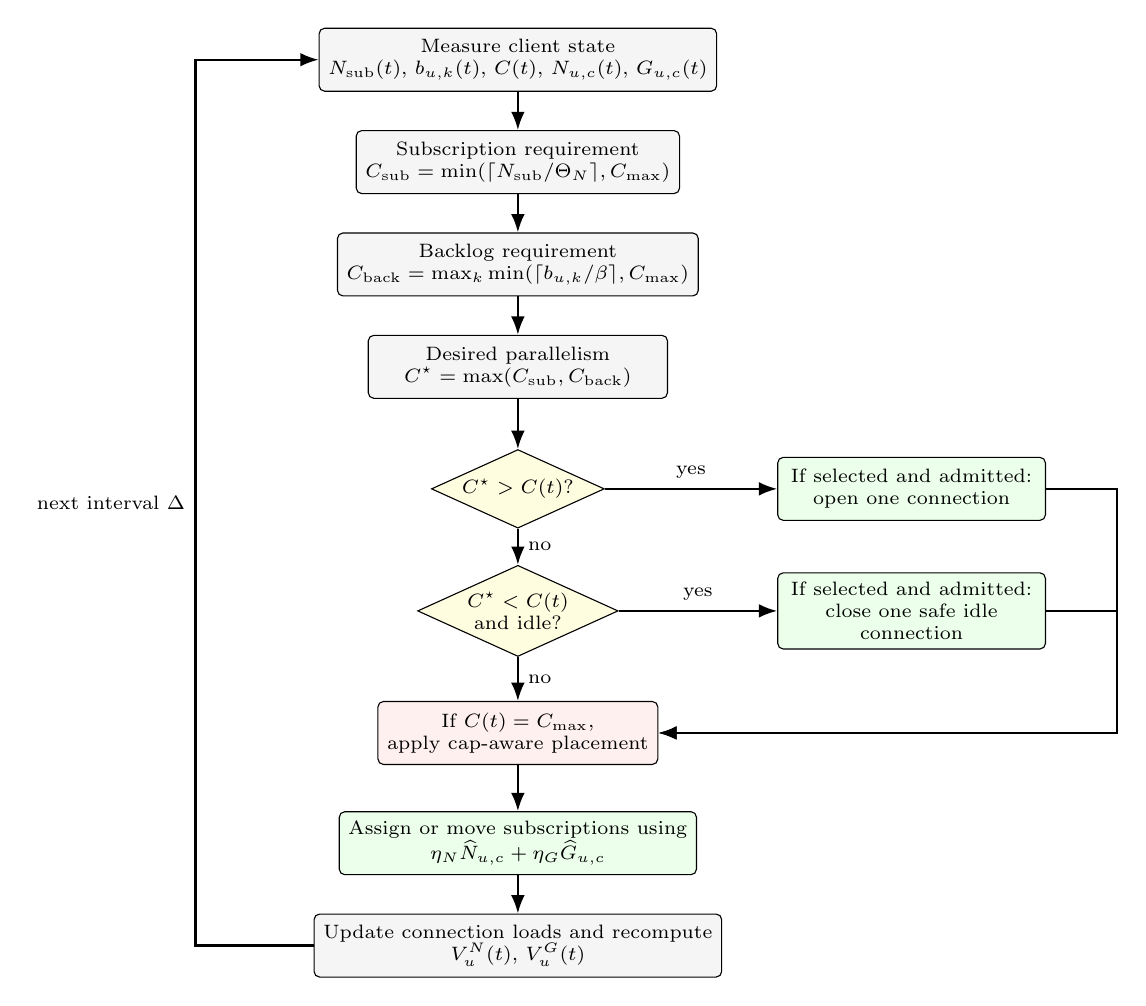
\begin{tikzpicture}[
		font=\scriptsize,
		node distance=9mm and 16mm,
		flowstep/.style={draw, rounded corners=2pt, align=center, minimum height=8mm, minimum width=38mm, fill=gray!8},
		decision/.style={draw, diamond, aspect=2.2, align=center, inner sep=1pt, fill=yellow!12},
		action/.style={draw, rounded corners=2pt, align=center, minimum height=8mm, minimum width=34mm, fill=green!8},
		guard/.style={draw, rounded corners=2pt, align=center, minimum height=8mm, minimum width=34mm, fill=red!6},
		arrow/.style={-Latex, thick}
	]
	\node[flowstep] (measure) at (0,0) {Measure client state\\$N_{\mathrm{sub}}(t)$, $b_{u,k}(t)$, $C(t)$, $N_{u,c}(t)$, $G_{u,c}(t)$};
	\node[flowstep] (subreq) at (0,-1.3) {Subscription requirement\\$C_{\mathrm{sub}}=\min(\lceil N_{\mathrm{sub}}/\Theta_N\rceil,C_{\max})$};
	\node[flowstep] (backreq) at (0,-2.6) {Backlog requirement\\$C_{\mathrm{back}}=\max_k \min(\lceil b_{u,k}/\beta\rceil,C_{\max})$};
	\node[flowstep] (desired) at (0,-3.9) {Desired parallelism\\$C^\star=\max(C_{\mathrm{sub}},C_{\mathrm{back}})$};
	\node[decision] (more) at (0,-5.45) {$C^\star>C(t)$?};
	\node[action] (open) at (5.0,-5.45) {If selected and admitted:\\open one connection};
	\node[decision] (less) at (0,-7.0) {$C^\star<C(t)$\\and idle?};
	\node[action] (close) at (5.0,-7.0) {If selected and admitted:\\close one safe idle\\connection};
	\node[guard] (cap) at (0,-8.55) {If $C(t)=C_{\max}$,\\apply cap-aware placement};
	\node[action] (assign) at (0,-9.95) {Assign or move subscriptions using\\$\eta_N\widehat{N}_{u,c}+\eta_G\widehat{G}_{u,c}$};
	\node[flowstep] (update) at (0,-11.25) {Update connection loads and recompute\\$V^N_u(t)$, $V^G_u(t)$};

	\draw[arrow] (measure) -- (subreq);
	\draw[arrow] (subreq) -- (backreq);
	\draw[arrow] (backreq) -- (desired);
	\draw[arrow] (desired) -- (more);
	\draw[arrow] (more.east) -- node[above] {yes} (open.west);
		\draw[arrow] (open.east) -- ++(0.9,0) |- (cap.east);
	\draw[arrow] (more) -- node[right] {no} (less);
	\draw[arrow] (less.east) -- node[above] {yes} (close.west);
		\draw[arrow] (close.east) -- ++(0.9,0) |- (cap.east);
	\draw[arrow] (less) -- node[right] {no} (cap);
	\draw[arrow] (cap) -- (assign);
	\draw[arrow] (assign) -- (update);
	\draw[arrow] (update.west) -- ++(-1.5,0) |- node[pos=0.25, left] {next interval $\Delta$} (measure.west);
	\end{tikzpicture}
	}
	\caption{Adaptive connection-scaling workflow. The client first computes the connection requirement induced by subscription density and the requirement induced by per-subscription backlog. The larger requirement determines the desired number of persistent connections, bounded by $C_{\max}$. If the cap is reached, the client assigns or moves subscriptions using a two-dimensional score that combines subscription-count pressure and backlog pressure. One DQL $a^{\mathrm{scale}+}$ decision creates at most one connection and then restores the subscription target through bounded receipt-gated reassociation.}
	\Description{Flowchart beginning with observed subscription and backlog state. Parallel branches calculate connection requirements from subscription density and queue backlog, merge them into a bounded desired connection count, then compare desired and current counts. The yes branches open or close persistent connections; otherwise the workflow performs cap-aware two-dimensional subscription placement and returns to monitoring.}
	\label{fig:scaling_workflow}
\end{figure*}
   

\subsection{Adaptive Parallel Connection Scaling - Algorithm}

\subsubsection{Mathematical Model}

Unlike server-level placement, which changes the pod reached by a connection,
connection scaling changes the amount of parallelism available to a client. In
subscription-driven messaging systems, too few persistent connections can force
many high-backlog subscriptions through the same processing path, increasing
latency and delaying acknowledgements.

The algorithms use the same backlog $b_{u,k}(t)$ and connection subscription
count $N_{u,c}(t)$ as the formal model. For compactness, the single-client
scaling counts below suppress the fixed client index $u$.

Let the client-side subscription population be
\begin{equation}
	N_{\mathrm{sub}}(t)=|\mathcal{K}_u(t)|,
\end{equation}
where $\mathcal{K}_u(t)$ is the set of active subscriptions maintained by
client $u$ at time $t$. Thus $N_{\mathrm{sub}}(t)$ counts subscriptions, not messages.

Let the current connection count be
\begin{equation}
	C(t)=|\mathcal{C}_u(t)|,
\end{equation}
where $\mathcal{C}_u(t)$ is the set of active persistent transport connections
used by client $u$ for message delivery at time $t$. Hence $C(t)$ is the
current number of usable STOMP/TCP/WebSocket-style delivery connections before
the scaling decision is applied. The retained statistics-only probe is not
counted in $C(t)$ unless it is promoted into a
persistent delivery connection.

The desired count $C^\star(t)$ can differ from the amount executed in one DQL
decision. Algorithm~\ref{alg:adaptive_parallel_scaling} computes the desired
parallelism, whereas one $a^{\mathrm{scale}+}$ option adds at most one connection. It
then moves whole subscriptions until no active connection exceeds $\Theta_N$,
or until no eligible move remains. A subscription has exactly one active
delivery binding outside the receipt-gated handoff interval; this mechanism does
not split one subscription queue across several connections.
Using the requirements defined below, the workflow abbreviates
$C_{\mathrm{back}}(t)=\max_{k\in\mathcal{K}_u(t)}C_k(t)$ and
$C^\star(t)=\max\{C_{\mathrm{sub}}(t),C_{\mathrm{back}}(t)\}$ for a nonempty subscription set.

We define:

\begin{itemize}
	\item $\Theta_N$ : maximum desired subscription count per connection
	\item $\beta$ : backlog threshold
	\item $C_{\max}$ : maximum allowable connections
\end{itemize}

The complete notation reference is collected in Appendix~\ref{app:notation}.

\subsubsection{Subscription-Based Scaling}

As the number of subscriptions increases, each connection must handle more message streams. To prevent overload, the desired number of connections is defined as:

\begin{equation}
	C_{\mathrm{sub}}(t) =
	\min\left(
	\left\lceil \frac{N_{\mathrm{sub}}(t)}{\Theta_N} \right\rceil,
	C_{\max}
	\right)
\end{equation}

Here $\Theta_N$ is a configured subscription-density threshold: it is the
maximum desired number of subscriptions assigned to one persistent connection
under normal operating conditions. It is not learned by DQL and is not the
DQL parameter vector $\theta$ used in $Q_\theta(o,a)$.

If:

\[
C_{\mathrm{sub}}(t) > C(t)
\]

the desired count exceeds the current count. The policy may request one
admissible scale-up action; the sizing calculation itself opens no sockets.

The count rule bounds mean subscription density when sufficient capacity is
available. A per-connection bound additionally requires the reassociations
to complete; the executor records whether that target was restored.

The sizing rule and the reassociation executor therefore have separate roles:
one requests enough sockets, and the other redistributes eligible subscriptions.


\subsubsection{Max-Cap Distribution Strategy}

When:

\[
C(t) = C_{\max}
\]

further scaling is restricted. In this scenario, newly arriving subscriptions are assigned using load-aware distribution.

Let:

\begin{equation}
	N_{u,c_j}(t)
\end{equation}

denote the number of subscriptions assigned to connection $c_j$.

New subscriptions are assigned to the connection with the lowest combined
subscription-count and backlog pressure:

\begin{equation}
	c^{\mathrm{place}} =
	\arg\min_{c_j \in \mathcal{C}_u(t)}
	\left(
	\eta_N \widehat{N}_{u,c_j}(t)
	+\eta_G \widehat{G}_{u,c_j}(t)
	\right)
\end{equation}

This greedy balancing strategy avoids assigning new subscriptions to a
connection that is already heavy either in subscription count or cumulative
subscription backlog.
Here $c^{\mathrm{place}}$ is the selected placement connection, while $c^\star$ is the
connection evaluated for migration. The hats on $N_{u,c_j}$ and $G_{u,c_j}$
denote normalized loads, not the normalized variances
$\widehat{V}^N_u$ and $\widehat{V}^G_u$.

\subsubsection{Backlog-Based Scaling}

Subscription backlog signals queued work, but its cause may lie in Pod service,
client acknowledgement capacity, or shared queue bandwidth. Scaling is useful
when additional connections can reach otherwise unused service capacity.

For subscription $k$, let backlog be:

\begin{equation}
	b_{u,k}(t)
\end{equation}

If:

\[
b_{u,k}(t) > \beta
\]

the configured backlog-pressure threshold has been crossed.

The required number of connections is:

\begin{equation}
	C_k(t) =
	\min\left(
	\left\lceil \frac{b_{u,k}(t)}{\beta} \right\rceil,
	C_{\max}
	\right)
\end{equation}

If:

\[
C_k(t) > C(t)
\]

backlog suggests additional parallelism. The selector still decides whether
to execute a bounded scaling action under the current guards.

The additional capacity can then receive eligible whole subscriptions from
loaded connections. Subscription $k$ itself remains active on exactly one
connection; its queue is not partitioned by this mechanism. Thus backlog-based
scaling can improve parallelism across a set of subscriptions, but it cannot
parallelize the delivery of one indivisible subscription queue by itself.



\subsubsection{Scaling Objective}

The objective of adaptive parallel connection scaling is to minimize backlog while respecting connection constraints:

\begin{equation}
	\min \sum_{k\in\mathcal{K}_u(t)} b_{u,k}(t)
\end{equation}

subject to:

\begin{equation}
	C(t) \le C_{\max}
\end{equation}

This represents a constrained parallel resource allocation problem.


\begin{algorithm}[htbp]
\small
\caption{Desired Connection Count (Sizing Only)}
\label{alg:adaptive_parallel_scaling}
\SetKwInOut{Input}{Input}
\SetKwInOut{Output}{Output}
\Input{Subscription set $\mathcal{K}_u(t)$, backlogs $b_{u,k}(t)$;
thresholds $\Theta_N,\beta$; hard cap $C_{\max}$}
\Output{Desired count $C^\star(t)$; no connection mutation}
$N_{\mathrm{sub}}(t)\leftarrow|\mathcal{K}_u(t)|$\;
$C_{\mathrm{sub}}(t)\leftarrow
\min\{\lceil N_{\mathrm{sub}}(t)/\Theta_N\rceil,C_{\max}\}$\;
$C_{\mathrm{back}}(t)\leftarrow0$\;
\ForEach{$k\in\mathcal{K}_u(t)$}{
 $C_k(t)\leftarrow\min\{\lceil b_{u,k}(t)/\beta\rceil,C_{\max}\}$\;
 $C_{\mathrm{back}}(t)\leftarrow\max\{C_{\mathrm{back}}(t),C_k(t)\}$\;
}
$C^\star(t)\leftarrow\max\{C_{\mathrm{sub}}(t),C_{\mathrm{back}}(t)\}$\;
\Return $C^\star(t)$ as decision context for the selector\;
\end{algorithm}

\subsection{Connection-Level Load Rebalancing - Algorithm}

\subsubsection{Motivation}

Adaptive connection scaling increases processing capacity as subscription count or backlog grows. Scaling alone, however, does not guarantee an even workload. New subscriptions, changing backlogs, and scaling decisions made at different times can leave some connections with far more subscriptions than others.

Such imbalance leads to:

\begin{itemize}
	\item Uneven CPU utilization
	\item Increased processing latency on overloaded connections
	\item Underutilized parallel capacity on lightly loaded connections
\end{itemize}

Therefore, a dedicated rebalancing mechanism is required to maintain fairness and stability across scaled connections.

\subsubsection{Load Distribution Model}

Connection load is represented by two variables. For connection $c$, $N_{u,c}(t)$
is the number of subscriptions assigned to the connection, and $G_{u,c}(t)$ is
the cumulative backlog of those subscriptions. The rebalancing controller
therefore monitors both $V^N_u(t)$ and $V^G_u(t)$ as defined in the problem
formulation.

High $V^N_u(t)$ means that subscription-management work is skewed across the
client's persistent connections. High $V^G_u(t)$ means that queue pressure is
skewed even if subscription counts look balanced. Either condition can degrade
delivery stability.

\subsubsection{Rebalancing Objective}

The local objective of connection-level rebalancing is:

\begin{equation}
	\min
	\left(
	\eta_N\widehat{V}^N_u(t)
	+\eta_G\widehat{V}^G_u(t)
	\right)
\end{equation}

subject to:

\begin{equation}
	1 \leq |\mathcal{C}_u(t)| \leq C_{\max}.
\end{equation}

This objective keeps both subscription-count skew and backlog skew under
control.

\subsubsection{Guarded Connection-Level Rebalancing Strategy}

The two rebalancing templates have separate admissibility conditions:

\begin{equation}
	\widehat{V}^N_u(t) > \gamma_N
	\quad \text{or} \quad
	\widehat{V}^G_u(t) > \gamma_G.
\end{equation}

The DQL policy, rather than Algorithm~\ref{alg:connection_rebalancing}, decides
whether the current observation calls for $a^{\mathrm{reb}N}$, $a^{\mathrm{reb}G}$, or another
action. If it selects $a^{\mathrm{reb}N}$, the executor moves one eligible subscription
from the connection with largest $N_{u,c}(t)$ to the connection with smallest
$N_{u,c}(t)$. If it selects $a^{\mathrm{reb}G}$, the executor chooses the subscription
whose reassociation from a high-backlog connection to a low-backlog connection
produces the largest predicted decrease in $V^G_u(t)$. The corresponding
threshold is then applied as a deterministic deployment guard. At most one
bounded reassociation is executed in a control interval. This limits repeated
back-and-forth moves and links the next reward to a clear action.

\begin{algorithm}[htbp]
	\small
	\caption{Guarded Executor for DQL-Selected Connection-Level Rebalancing}
	\label{alg:connection_rebalancing}
	\SetAlgoLined
	\SetKwInOut{Input}{Input}
	\SetKwInOut{Output}{Output}
	\Input{Selected template $a_u(t)\in\{a^{\mathrm{reb}N},a^{\mathrm{reb}G}\}$; connections $\mathcal{C}_u(t)$; subscription counts $N_{u,c}$; connection backlogs $G_{u,c}$; thresholds $\gamma_N,\gamma_G$}
	\Output{Updated assignment, or the unchanged assignment when the selected template is inadmissible}
	Compute $\widehat{V}^N_u(t)$ and $\widehat{V}^G_u(t)$\;
	\eIf{$a_u(t)=a^{\mathrm{reb}N}$}{
		\If{$\widehat{V}^N_u(t)\leq\gamma_N$}{
			\Return unchanged assignment \tcp*[r]{Guarded no-op}
		}
		$c_h \leftarrow \arg\max_{c\in\mathcal{C}_u(t)}N_{u,c}(t)$\;
		$c_l \leftarrow \arg\min_{c\in\mathcal{C}_u(t)}N_{u,c}(t)$\;
		Select an eligible movable subscription $k$ from $c_h$ using a stable tie-break\;
	}{
		\If{$\widehat{V}^G_u(t)\leq\gamma_G$}{
			\Return unchanged assignment \tcp*[r]{Guarded no-op}
		}
		$c_h \leftarrow \arg\max_{c\in\mathcal{C}_u(t)}G_{u,c}(t)$\;
		$c_l \leftarrow \arg\min_{c\in\mathcal{C}_u(t)}G_{u,c}(t)$\;
		Select eligible $k$ on $c_h$ maximizing the predicted decrease in $V^G_u(t)$\;
	}
	\If{$c_h=c_l$ or no eligible $k$ exists}{
		\Return unchanged assignment \tcp*[r]{Guarded no-op}
	}
	Reassociate $k$ from $c_h$ to $c_l$ using the guarded executor\;
	Update $N_{u,c_h},N_{u,c_l},G_{u,c_h},G_{u,c_l}$\;
	\Return updated assignment\;
\end{algorithm}

Algorithm~\ref{alg:connection_rebalancing} carries out the selected action;
it is not a second policy. In particular, it never compares
$\widehat{V}^N_u(t)$ with $\widehat{V}^G_u(t)$ to decide which objective will
dominate. These normalized quantities can have different observed
distributions even though both are bounded. The selected DQL template is the
stored action, while the reward and next observation reflect the executor
outcome, including a guarded no-op. The learned value therefore accounts for whether an action can be executed,
without introducing a second rebalancing policy.


\subsection{DQL-Based Rebalancing and Placement Algorithm}
This section presents the client-driven DQL controller under the observability
constraints described above. Each client keeps a statistics cache with two sources.
Active connections report their current pod's tuple every $\Delta=10$ seconds.
An authenticated, statistics-only probe provides the other source. The load
balancer assigns its endpoint when the socket is established. The
client retains that socket and candidate-pod identity until promotion, expiry,
or recycling while periodically obtaining the tuple in (\ref{eq:pod_stats}). The controller then
uses the observation vector in (\ref{eq:dql_observation}) to select one of the
action templates in (\ref{eq:dql_actions}).

\begin{figure*}[!htbp]
\centering
\begin{subfigure}{\textwidth}
\centering
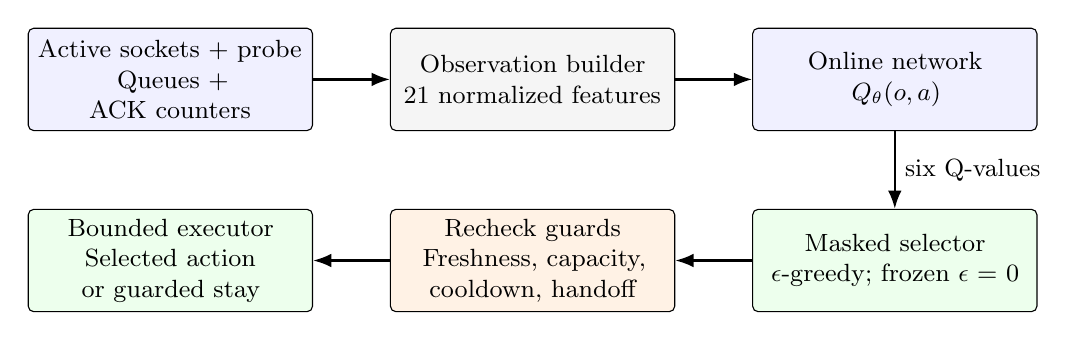
\begin{tikzpicture}[
 font=\small,
 module/.style={draw,rounded corners=2pt,align=center,text width=34mm,minimum height=13mm,inner sep=3pt},
 arrow/.style={-Latex,thick}]
 \node[module,fill=blue!6] (measure) at (0,0) {Active sockets + probe\\Queues + ACK counters};
 \node[module,fill=gray!8] (obs) at (4.6,0) {Observation builder\\21 normalized features};
 \node[module,fill=blue!6] (online) at (9.2,0) {Online network\\$Q_\theta(o,a)$};
 \node[module,fill=green!7] (policy) at (9.2,-2.3) {Masked selector\\$\epsilon$-greedy; frozen $\epsilon=0$};
 \node[module,fill=orange!10] (guard) at (4.6,-2.3) {Recheck guards\\Freshness, capacity,\\cooldown, handoff};
 \node[module,fill=green!7] (execute) at (0,-2.3) {Bounded executor\\Selected action\\or guarded stay};
 \draw[arrow] (measure) -- (obs);
 \draw[arrow] (obs) -- (online);
 \draw[arrow] (online) -- node[right]{six Q-values} (policy);
 \draw[arrow] (policy) -- (guard);
 \draw[arrow] (guard) -- (execute);
\end{tikzpicture}
\caption{Runtime decision path. The target network is not on this path.}
\end{subfigure}

\medskip
\begin{subfigure}{\textwidth}
\centering
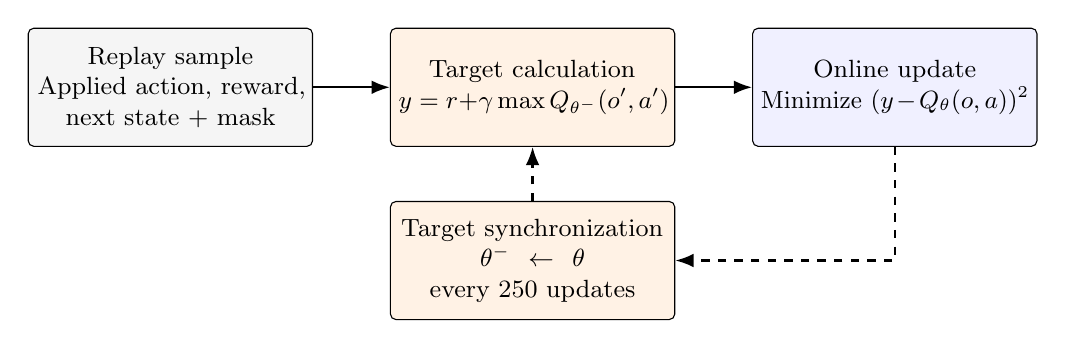
\begin{tikzpicture}[
 font=\small,
 module/.style={draw,rounded corners=2pt,align=center,text width=34mm,minimum height=15mm,inner sep=3pt},
 arrow/.style={-Latex,thick}, learn/.style={-Latex,thick,dashed}]
 \node[module,fill=gray!8] (replay) at (0,0) {Replay sample\\Applied action, reward,\\next state + mask};
 \node[module,fill=orange!10] (target) at (4.6,0) {Target calculation\\$y=r+\gamma\max Q_{\theta^-}(o',a')$};
 \node[module,fill=blue!6] (update) at (9.2,0) {Online update\\Minimize $(y-Q_\theta(o,a))^2$};
 \node[module,fill=orange!10] (copy) at (4.6,-2.2) {Target synchronization\\$\theta^-\leftarrow\theta$\\every 250 updates};
 \draw[arrow] (replay) -- (target);
 \draw[arrow] (target) -- (update);
 \draw[learn] (update.south) |- (copy.east);
 \draw[learn] (copy.north) -- (target.south);
\end{tikzpicture}
\caption{Training path for the evaluated v3 learner. Frozen evaluation disables updates.}
\end{subfigure}
\caption{DQL selection and learning are separate from the shared guarded
executor. Solid arrows show runtime or training data flow; dashed arrows copy
parameters to the target network. Only the online network ranks live actions.
The target network stabilizes the next-state value used during training.}
\Description{Two readable panels. The runtime path goes from telemetry through
a 21-feature observation and online Q-network to masked selection, guard
rechecks, and execution. The training path goes from replay to target
calculation and online loss minimization, with a separate periodic target copy.}
\label{fig:dql_message_flow}
\end{figure*}

\begin{figure*}[!htbp]
\centering
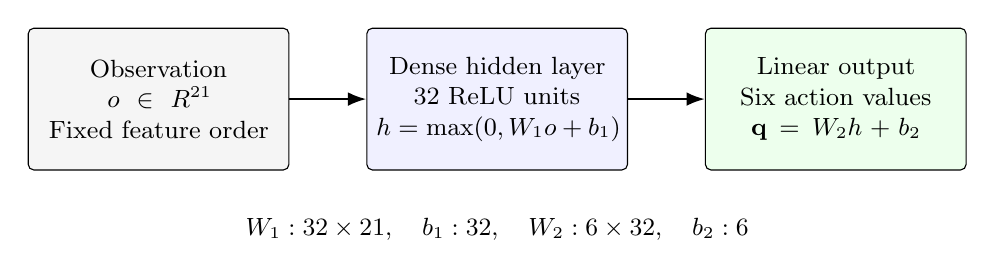
\begin{tikzpicture}[
 font=\small,
 module/.style={draw,rounded corners=2pt,align=center,text width=31mm,minimum height=18mm,inner sep=3pt},
 arrow/.style={-Latex,thick}]
 \node[module,fill=gray!8] (input) at (0,0) {Observation\\$o\in\mathbb{R}^{21}$\\Fixed feature order};
 \node[module,fill=blue!6] (hidden) at (4.3,0) {Dense hidden layer\\32 ReLU units\\$h=\max(0,W_1o+b_1)$};
 \node[module,fill=green!7] (output) at (8.6,0) {Linear output\\Six action values\\$\mathbf{q}=W_2h+b_2$};
 \draw[arrow] (input) -- (hidden);
 \draw[arrow] (hidden) -- (output);
 \node[align=center,font=\small] at (4.3,-1.65)
 {$W_1:32\times21,\quad b_1:32,\quad W_2:6\times32,\quad b_2:6$};
\end{tikzpicture}
\caption{The evaluated Q-network: 21 input features, one fully connected
32-unit ReLU layer, and six linear outputs. Each arrow denotes a dense matrix
operation, not a sparse connection between individual neurons. There are no
separate learned feature encoders. The online and target networks have this
same architecture and different parameter-update roles.}
\Description{Three separated modules show the actual dense 21--32--6 network.
The input feeds one ReLU hidden layer, which feeds six linear Q-values.
Weight and bias dimensions appear below the modules.}
\label{fig:dql_q_network_tree}
\end{figure*}

In Figure~\ref{fig:dql_q_network_tree}, $o$ abbreviates $o_u(t)$ and
$\theta=(W_1,b_1,W_2,b_2)$. There are $902$ trainable scalar parameters in
each network. The output order is
$(a^{\mathrm{stay}},a^{\mathrm{reb}N},a^{\mathrm{reb}G},
a^{\mathrm{scale}+},a^{\mathrm{scale}-},a^{\mathrm{mig}})$.
Grouping features by meaning in (\ref{eq:dql_observation}) does not introduce
additional neural layers. Table~\ref{tab:dql-configuration} gives the
evaluated v3 configuration; Appendix~\ref{app:feature-order} gives the exact
input order and normalization.

\begin{table}[!htbp]
\centering\small
\caption{Configuration of the v3 DQL policy used in the reported holdout,
scale-out simulator, and October live trial. Later learner variants are
reported separately in Appendix~\ref{app:action-diagnostics}.}
\Description{A reproducibility table of network dimensions, training settings,
reward weights, exploration, and frozen evaluation settings.}
\label{tab:dql-configuration}
\begin{tabular}{p{0.38\textwidth}p{0.54\textwidth}}
\toprule
Setting & Value\\
\midrule
Network; optimizer & Dense 21--32--6; ReLU hidden, linear output; mini-batch gradient descent\\
Discount; learning rate & $\gamma=0.99$; $\alpha=0.001$\\
Replay; batch; target copy & Uniform replay, capacity 5,000; batch 16; copy every 250 updates\\
Bootstrap; loss & Target-network maximum over admitted actions; squared TD error\\
Training budget & 10,000 transitions per candidate; 9,985 updates after batch warm-up\\
Training exploration & $\epsilon_0=1$, multiplier $\exp(\log(0.05)/10{,}000)$; floor 0.05\\
Reward weights $(\lambda_1,\ldots,\lambda_7)$ & $(0.20,0.15,0.20,0.15,0.10,0.05,0.15)$\\
Pressure weights $(\omega_X,\omega_B,\omega_H,\omega_R)$ & $(0.30,0.25,0.20,0.25)$\\
Imbalance weights & $\eta_N=\eta_G=0.5$\\
Frozen evaluation & $\epsilon=0$; no model or replay updates; checkpoint hash retained\\
\bottomrule
\end{tabular}
\end{table}

\subsubsection{Reward-Based Learning}

For every observed pod $i\in\mathcal{O}_u(t)$, the client computes pod pressure
$P_i(t)$ from (\ref{eq:pod_pressure}). This pressure explicitly penalizes both
pod subscription count and pod cumulative backlog. The subscription-count term
captures the observed reliability degradation of pods with excessive
subscription-management load, while the backlog term captures queue
accumulation. The threshold $H_i$ is used only as a capacity-normalized pressure
term; it is not interpreted as the actual client-side drain rate.

After action execution, the client computes reward $R_u(t)$ using
(\ref{eq:deployable_reward}). This reward includes local backlog, backlog
growth, local connection imbalance, migration cost, connection cost, pod
pressure, and effective client-side throughput. Hence the learned policy is
trained using information that the client can actually observe at runtime.

\subsubsection{Exploration, Hysteresis, and Migration}

Let $\mathcal{A}^{\mathrm{adm}}_u(t)\subseteq\mathcal{A}$ contain only the templates
that pass the current freshness, capacity, cooldown, and handoff guards. The
DQL policy uses epsilon-greedy exploration over this masked set:
\begin{equation}
	a_u(t)=
	\begin{cases}
		\text{Uniform}(\mathcal{A}^{\mathrm{adm}}_u(t)), & \text{w.p. } \epsilon,\\
		\arg\max_{a\in\mathcal{A}^{\mathrm{adm}}_u(t)} Q_\theta(o_u(t),a), & \text{w.p. } 1-\epsilon.
	\end{cases}
\end{equation}
The exploration probability decreases during training. Frozen validation and
deployment policies use $\epsilon=0$. This prevents unreviewed exploratory
changes during evaluation. Online exploration would require a separate
safety study. Migration is
executed only when the selected action is $a^{\mathrm{mig}}$ and the retained probe
candidate improves the estimated value by a hysteresis threshold:
\begin{equation}
	Q_\theta(o_u(t),a^{\mathrm{mig}}) >
	Q_\theta(o_u(t),a^{\mathrm{stay}})+\delta.
\end{equation}
This threshold prevents oscillatory migrations caused by small or stale
statistical differences. It does not choose the probe endpoint: the Kubernetes
load balancer already fixed that endpoint when the probe socket was opened.
Passing this value test is necessary but not sufficient. The executor also
checks telemetry freshness, target capacity, source--target separation, cooldown,
and the absence of a conflicting handoff. As a result, most probes
can remain telemetry-only and may expire or be recycled without carrying a
subscription.

\begin{algorithm}[!htbp]
	\small
	\caption{DQL-Based Client-Side Persistent Transport Rebalancing}
	\label{alg:dql_rebalancing}
	\SetAlgoLined
	\SetKwInOut{Input}{Input}
	\SetKwInOut{Output}{Output}
	\Input{Replay buffer $\mathcal{D}$; online network $Q_\theta$; target network $Q_{\theta^-}$\\
	Observed pod set $\mathcal{O}_u(t)$ and its cached tuples $y_i(t)$; retained authenticated probe and endpoint $i^{\mathrm{probe}}_u(t)$\\
	Exploration probability $\epsilon$; discount factor $\gamma$; migration threshold $\delta$; target $\Theta_N$; hard cap $C_{\max}$}
	\Output{Adaptive rebalancing, scaling, and migration decisions}
	$t\leftarrow0$; use the active delivery pool and one authenticated probe\;
	Load the declared checkpoint; initialize networks/replay only for new training\;
	\While{client is active}{
		Update the pod cache from active and retained-probe telemetry\;
		Measure per-subscription backlogs, connection loads, throughput, and acknowledgements\;
		Construct observation $o_u(t)$ using (\ref{eq:dql_observation})\;
		Construct the masked admissible set $\mathcal{A}^{\mathrm{adm}}_u(t)$ from freshness, capacity, cooldown, and handoff guards\;
		$a_u(t) \leftarrow \epsilon\text{-greedy}(Q_\theta,o_u(t),\mathcal{A}^{\mathrm{adm}}_u(t))$\;
		\eIf{$a_u(t)\in\{a^{\mathrm{reb}N},a^{\mathrm{reb}G}\}$}{
			Instantiate the selected template using Algorithm~\ref{alg:connection_rebalancing}\;
		}{
			\eIf{$a_u(t)=a^{\mathrm{mig}}$}{
				\eIf{probe and handoff guards pass, including the hysteresis test}{
					Promote the same retained probe and execute the receipt-gated handoff in Section~\ref{sec:probe_handoff}\;
					Open a new statistics-only probe through the load balancer after handoff\;
				}{
					Record a guarded no-op; preserve source ownership and probe role\;
				}
			}{
				\eIf{$a_u(t)=a^{\mathrm{scale}+}$}{
					\eIf{capacity and subscription-demand guards still pass}{
						Open one connection; apply receipt-gated $a^{\mathrm{reb}N}$ moves until $\max_{c\in\mathcal{C}_u(t)}N_{u,c}(t)\leq\Theta_N$ or no move exists\;
						Record move count and target-restored status\;
					}{
						Record a guarded no-op\;
					}
				}{
					\eIf{$a_u(t)=a^{\mathrm{scale}-}$}{
						Close one safe idle connection after rechecking its guard\;
					}{
						Preserve the current topology for $a^{\mathrm{stay}}$\;
					}
				}
			}
		}
		Observe reward $R_u(t)$ from (\ref{eq:deployable_reward}) and next observation $o_u(t+1)$\;
		Log the applied action, reward, next observation, and guard outcome\;
		\If{training is enabled and the transition is valid}{
			Store the applied-action transition and next-state mask in $\mathcal{D}$\;
			Update from a mini-batch using (\ref{eq:dql_loss}); synchronize the target when due\;
		}
		Wait $\Delta$; $t\leftarrow t+1$\;
	}
	\Return policy and recorded action outcomes\;
\end{algorithm}

\begin{align}
	\text{computeReward}(i,u,t)=R_u(t) =
	&-\lambda_1\widehat{B}_u
	-\lambda_2\widehat{\mathrm{Grow}}_u \nonumber\\
	&-\lambda_3 P_i
	-\lambda_4 V_u \nonumber\\
	&-\lambda_5 M_u
	-\lambda_6\widehat{C}_u
	+\lambda_7\widehat{T}_u
	\label{eq:reward_function}
\end{align}
The epsilon-greedy rule is therefore used as the exploration mechanism inside
DQL, not as the main learning model. Unlike a stateless bandit controller, DQL
can learn delayed effects. Scale-up with subscription restoration has an
immediate connection and reassociation cost but may later reduce backlog growth.
Migration may have an immediate penalty but later avoid an unreliable pod with
too many subscriptions. A rebalancing move may help only after queues have had
time to drain.



\subsection{Hierarchical Optimization Structure}

The resulting control structure has two complementary levels:

\begin{enumerate}
	
	\item \textbf{Server-Level Optimization:}
	The DQL controller selects migration only when the observed pod statistics
	and local client state suggest that moving to a candidate pod is likely to
	improve long-term reward after migration cost.
	
	\item \textbf{Connection-Level Optimization:}
	The same policy decides when to rebalance subscriptions, increase or
	decrease connection parallelism, or leave the current assignment unchanged.
	
\end{enumerate}

This hierarchical design enables simultaneous optimization of:

\begin{itemize}
	\item Inter-server load distribution
	\item Intra-client parallelism
	\item Subscription fairness
	\item Backlog reduction
\end{itemize}

The learned component does not create arbitrary subscription assignments.
It chooses bounded action templates that the client can execute and check
against deployment guards.

\section{Oracle Cloud Cluster Deployment Experiment}
\label{sec:mumbai-experiment}

We deployed the connection-replacement mechanism in an Oracle Cloud cluster
running Kubernetes in a development environment and first exercised it with 20,000
registered subscriptions. This initial experiment
measures live probe promotion, subscription reassociation, handoff timing, and
post-migration topology. The controlled scale-out and policy comparisons in
Section~\ref{sec:locked-evidence} use a simulator and are reported separately.
Sections~\ref{sec:mumbai-startup} and~\ref{sec:live-dql-scaleout} report
separate isolated trials, including selective DQL migration during delivery
and a one-to-four-Pod scale-out sequence.

\subsection{Deployment and Execution}

The deployment contained ten subscriber-service pods. Ten client processes
each maintained five active persistent connections, with 400 subscriptions per
connection, and one additional subscription-free probe. The inventory had
four event-type groups, each with 5,000 subscriptions. Every client loaded the
same frozen DQL checkpoint, with exploration disabled and no training updates
during evaluation. The deployed action profile admitted rebalancing and
migration but masked connection scale-up and scale-down.

Each client could execute at most one guarded connection migration. A selected
probe was promoted only after telemetry and execution checks passed. The
executor then reassociated the source connection's 400 subscriptions, drained
in-flight delivery, retired the source socket, and opened a fresh
subscription-free probe. Subscription receipts and server-reported counts
were checked against the client assignment. After execution, each process
held its topology for 1,800 seconds and checked it again before shutdown.
The statistical unit is one deployment run, containing ten client migrations.

\begin{table}[t]
  \caption{Measured Oracle Cloud cluster deployment results. Handoff and drain statistics
  summarize ten executed connection migrations. Drain wait is part of handoff
  time, not an additional independent interval.}
  \Description{Live experiment with ten pods, twenty thousand subscriptions,
  ten successful connection replacements, four thousand moved subscriptions,
  and exact final topology in all ten clients. Handoff median is 14.498 seconds;
  drain-wait median is 7.347 seconds.}
  \label{tab:mumbai-live-results}
  \centering
  \small
  \begin{tabular}{p{0.60\linewidth}r}
    \toprule
    Measurement & Observed value \\
    \midrule
    Subscriber-service pods / client processes & 10 / 10 \\
    Registered and attached subscriptions & 20,000 \\
    Active persistent connections / probes & 50 / 10 \\
    Executed full-connection migrations & 10 \\
    Subscriptions moved per migration / total & 400 / 4,000 \\
    Handoff time: minimum / median / maximum (s) & 7.898 / 14.498 / 101.563 \\
    Drain wait: minimum / median / maximum (s) & 1.264 / 7.347 / 92.450 \\
    Exact final topologies after 1,800 s & 10/10 \\
    Recorded deliveries / processed and acknowledged & 114,986 / 113,149 \\
    Processing failures / ACK failures / NACK failures & 0 / 0 / 0 \\
    Recorded duplicate candidates & 0 \\
    Independent pod samples / collection errors & 310 / 0 \\
    Pod restart increase during observation & 0 \\
    \bottomrule
  \end{tabular}
\end{table}

\subsection{Observed Handoff and Topology}

Table~\ref{tab:mumbai-live-results} shows that all ten clients replaced one
active connection and moved its full subscription set. In every case, the
destination was the retained probe, the other four active connections remained
in place, and the replacement probe had no subscriptions. The final checks
confirmed all 2,000 subscriptions and five active connections in each client
after the 30-minute hold. Thus, 4,000 subscriptions changed their transport
association while the complete 20,000-subscription client population remained
accounted for.

Handoff duration ranged from 7.898 to 101.563 seconds, with a median of
14.498 seconds. The corresponding source-drain waits ranged from 1.264 to
92.450 seconds, with a median of 7.347 seconds. The range is important:
replacement time includes waiting for outstanding work, not just opening
a socket. This run deliberately used eight processing workers
and a two-second processing delay per event in each client. Those settings
exercise handoff under a bounded client drain rate. The endpoint is handoff
behavior under this processing limit, rather than maximum Pod throughput.

\begin{figure}[!htbp]
  \centering
  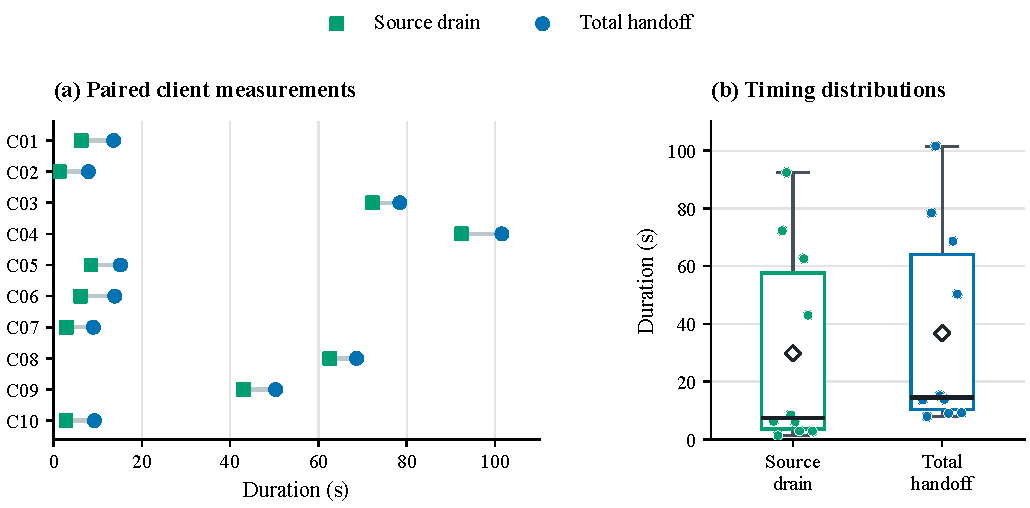
\includegraphics[width=\textwidth]{figures/mumbai-handoff-boxplots.pdf}
  \caption{Measured Oracle Cloud cluster migration timing. Left: paired source-drain and
  total-handoff durations for each of the ten client migrations. Right:
  quartile boxes with median lines, mean diamonds, and all ten observations;
  whiskers extend to observations within 1.5 interquartile ranges. These are
  ten migrations in one cluster run, not ten independent cluster trials.}
  \Description{Paired duration markers and box plots show source drain and
  total handoff for ten clients. Longer handoffs coincide with longer source
  drain waits. Drain is a component of
  total handoff, not an additional duration.}
  \label{fig:mumbai-handoff-distributions}
\end{figure}
\FloatBarrier

Figure~\ref{fig:mumbai-handoff-distributions} retains the pairing that a
summary median cannot show. For client $u$, the interval between its two
markers is $T^{\mathrm{handoff}}_u-T^{\mathrm{drain}}_u$, the measured non-drain remainder of
the handoff; it is not an estimate of network latency alone. The box extends
from the sample's first to third quartile, so the interquartile range describes
the central half of the timings. All points, including the long-duration
observations, remain visible. Longer handoffs coincide with longer source
drains, consistent with the receipt-gated mechanism waiting for outstanding
work. These are within-run timing distributions; their scope is the observed
deployment, without a between-deployment confidence interval.

An independent collector retained 31 observations of each of the ten pods
over approximately 2,422 seconds. All pods remained Ready, with unchanged
pod, image, and process identities and no restart increase. These observations
establish operational continuity over this observation period. Long-term
availability is outside the measurement window.

\subsection{Event Accounting and Interpretation}

The clients recorded 114,986 deliveries and 113,149 processed and acknowledged
events, with no recorded processing, acknowledgement, or negative-
acknowledgement failures. The final difference is 1,837 deliveries whose
eventual status is not resolved by these counters. Zero duplicate candidates
describes the configured observation window, rather than an exactly-once
delivery guarantee. The run consumed existing queued work without a matched
static-policy workload. Its contribution is measured probe-based connection
replacement with 20,000 subscriptions: subscription reassociation, source
retirement, and the connection layout after the hold period. Its endpoints
are handoff execution and topology retention, not a comparative backlog-drain
rate.

The private evidence archive retains the frozen-policy and inventory hashes,
per-client decision and topology records, delivery counters, and independent
pod observations. A recursive manifest covers 134 files; aggregate values in
Table~\ref{tab:mumbai-live-results} come from the active-execution gate and
pod-observation summaries, not from simulator output.

\subsection{Concentrated Placement and Startup Under Load}
\label{sec:mumbai-startup}

We conducted a separate Oracle Cloud cluster experiment with an isolated subscriber
Deployment and Service to examine what happens when persistent TCP connections remain on one Pod. In an initial 4,000-subscription static calibration, ten delivery
connections and two probes terminated on one Pod. Adding three Ready Pods did
not relocate these sockets: the source retained all twelve established
connections, while each added Pod had none. The clients nevertheless received
and acknowledged events while subscription activation was still progressing.
Full activation took approximately 1,398.4 seconds; the completed run reconciled
137,008 observed deliveries with confirmed ACKs. This shows the difference between having server capacity and reaching it
through existing persistent connections.

A later frozen-DQL test used 2,000 other subscriptions, divided
equally among four event-type groups. One client attached five connections,
each carrying 400 subscriptions, to the single source Pod. Three destination
Pods became Ready before standby bindings were activated. The client used
32 processing workers without an artificial processing delay, ten message
permits per subscription, and a window of 32 outstanding activation requests.
Exact lifecycle records used batched SQLite transactions with FULL
synchronization and a mandatory flush at measurement and closure boundaries.
The earlier calibration used a different subscription population and recorder
settings. The two timing records are therefore reported as separate
experiments rather than a matched static-policy comparison.

\begin{table}[!htbp]
  \caption{Measured isolated Oracle Cloud cluster connection-rebalancing qualification.
  These values describe one live run, distinct from the earlier
  20,000-subscription deployment.}
  \Description{Four available Pods, two thousand subscriptions, five active
  connections, three migrations of four hundred subscriptions, and exact
  reconciliation of seventy-three thousand six hundred thirty-nine observed
  deliveries. The source population falls from two thousand to eight hundred.}
  \label{tab:mumbai-isolated-recovery}
  \centering
  \small
  \begin{tabular}{p{0.65\linewidth}r}
    \toprule
    Measurement & Observed value \\
    \midrule
    Available Pods / subscribed Pods before and after & 4 / 1 and 3 \\
    Subscriptions / active connections / probe & 2,000 / 5 / 1 \\
    Time to 50\% / 90\% / full activation (s) & 238.066 / 388.139 / 426.305 \\
    Committed connection migrations / subscriptions moved & 3 / 1,200 \\
    Source subscriptions before / after & 2,000 / 800 \\
    Final subscribed-Pod populations & 800, 800, 400 \\
    Handoff times, in execution order (s) & 10.878, 10.992, 10.648 \\
    Source-drain waits, in execution order (s) & 6.069, 6.174, 6.848 \\
    Delivered / processed / receipt-confirmed ACKs & 73,639 / 73,639 / 73,639 \\
    Unresolved observed attempts at closure & 0 \\
    Recorded ACK failures / duplicate candidates & 0 / 0 \\
    \bottomrule
  \end{tabular}
\end{table}

The frozen controller committed three complete connection replacements,
each moving 400 subscriptions through a retained probe. The source population
fell from 2,000 to 800, a reduction of
$(2{,}000-800)/2{,}000=60\%$. Two destination Pods acquired 400 and 800
subscriptions. The active-connection count remained five, and all 2,000
subscriptions were confirmed in the final topology after the two-minute hold.
The migrations therefore changed which Pods served these subscriptions
without increasing the client's active-connection count.

\begin{figure}[!htbp]
  \centering
  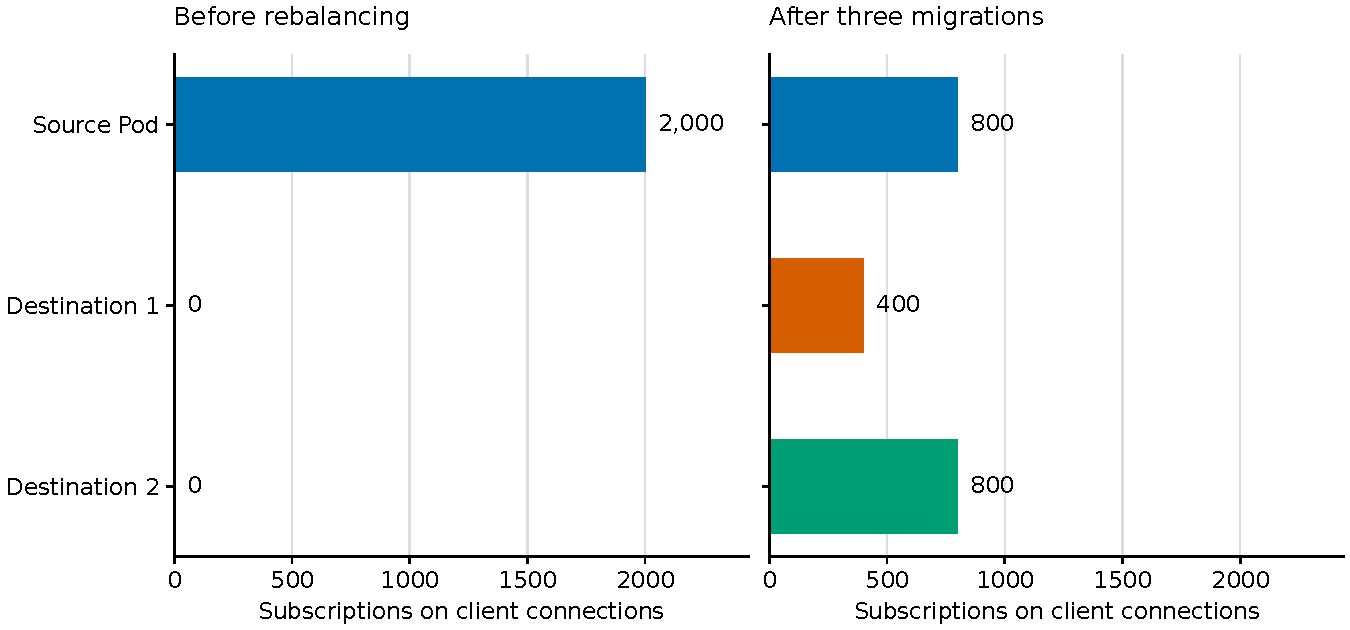
\includegraphics[width=\textwidth]{figures/observed-pod-redistribution.pdf}
  \caption{Verified client subscription placement before and after three
  frozen-DQL connection migrations in the Oracle Cloud cluster. Bars aggregate the client's
  receipt-confirmed bindings by serving Pod. Initial zeros mean no bindings
  belonging to this client, not a measurement of every cluster subscription.
  Both panels account for the same 2,000 subscriptions and five connections.}
  \Description{The initial source has two thousand subscriptions. After
  rebalancing it has eight hundred; two destinations have four hundred and
  eight hundred. No subscription is removed from the population.}
  \label{fig:mumbai-isolated-placement}
\end{figure}
\FloatBarrier

Figure~\ref{fig:mumbai-isolated-placement} shows the main operational effect:
newly available capacity becomes reachable by moving subscription-bearing
connections. It reports verified connection endpoints, rather than estimating changes
between observations. A probe was first resampled because it did not
offer an admissible improvement. Eleven later decision intervals selected
stay while backlog telemetry was incomplete; migration resumed when the
observation checks passed. The online and target network parameters remained
identical to the loaded checkpoint, while valid transitions were retained.

\subsubsection{Activation and Delivery Coexistence}

For subscription $k$, let $t_k^{\mathrm{send}}$ be activation submission time and $t_k^{\mathrm{ready}}$ its
successful receipt time, relative to the start of activation. At elapsed
time $s$ in seconds, the cumulative completion count is
$A^{\mathrm{act}}(s)=\sum_{k=1}^{2000}\mathbf{1}\{t_k^{\mathrm{ready}}\leq s\}$,
and $2000-A^{\mathrm{act}}(s)$ is the pending count. This separates attachment from
confirmed activation and makes startup delay visible even while events flow.
The 50th, 90th and 100th completion percentiles were 238.066, 388.139 and
426.305 seconds, respectively. No activation retry was needed in this run.

\begin{figure}[!htbp]
  \centering
  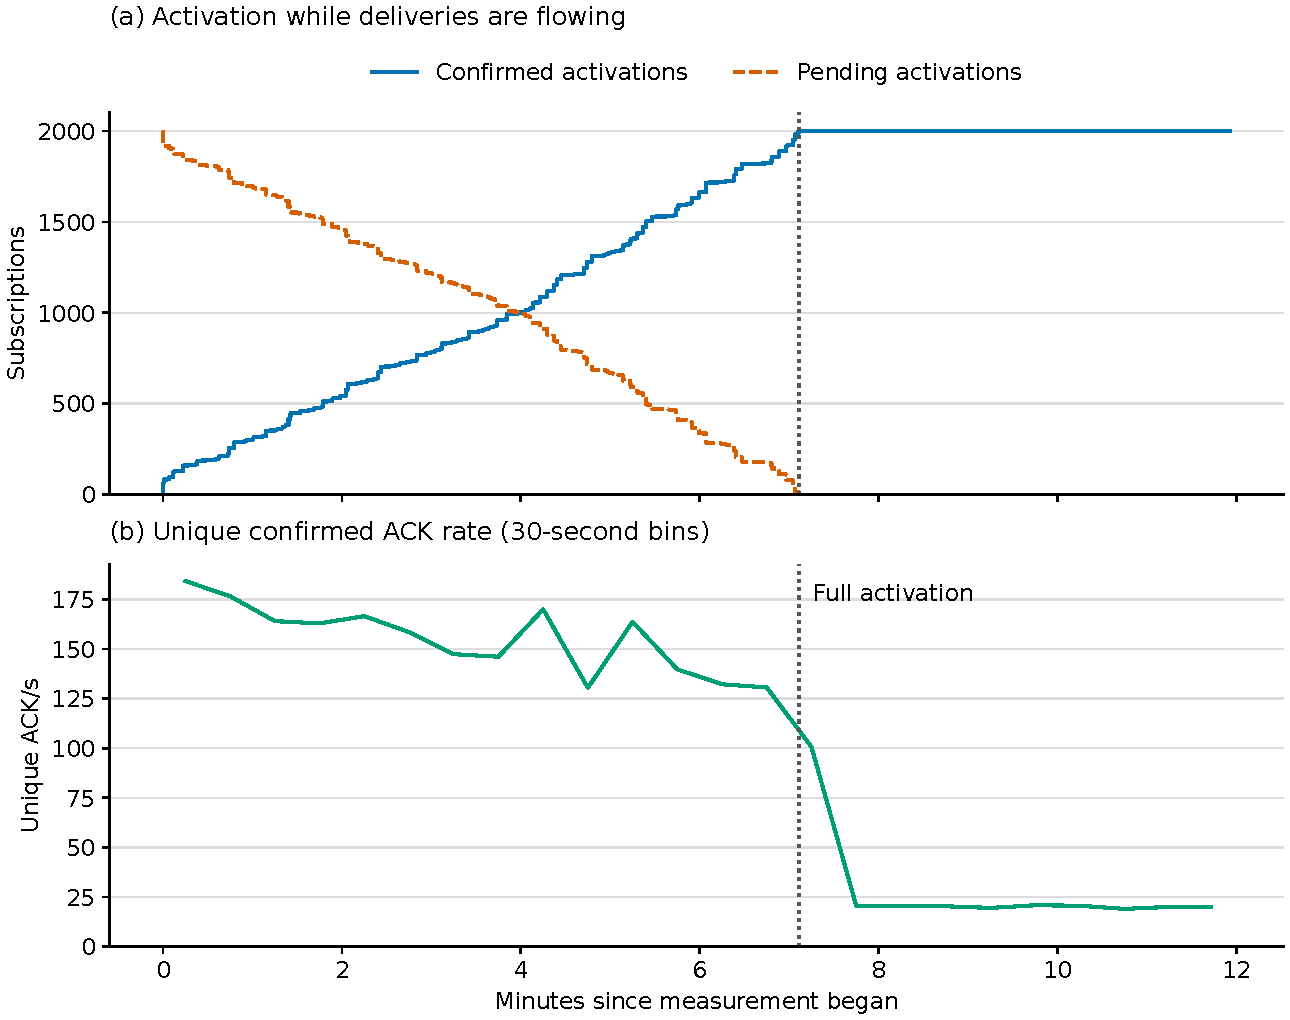
\includegraphics[width=0.94\textwidth]{figures/activation-and-ack-rate.pdf}
  \caption{Activation and acknowledged delivery in the isolated Oracle Cloud cluster run.
  Top: confirmed and pending activation counts. Bottom: distinct observed
  subscription--message pairs whose first successful ACK receipt occurs in
  each 30-second bin, divided by that bin's actual duration. The dotted line
  marks full activation. DQL decisions start after this line.}
  \Description{Activation rises to two thousand while pending activations
  fall to zero. ACKs arrive throughout startup. The later delivery rate falls
  as the consumed workload changes; the curve is not a matched throughput
  comparison with a static policy.}
  \label{fig:mumbai-live-activation}
\end{figure}
\FloatBarrier

Figure~\ref{fig:mumbai-live-activation} retains the startup interval rather
than treating it as discarded warm-up. Of 73,587 distinct first ACKs inside
the 716.017-second measurement window, 66,400 occurred before full activation.
A further 52 attempts completed during shutdown, bringing final reconciled
deliveries to 73,639. The rate curve describes consumption of existing queued
work. It describes startup and workload drainage rather than constant-offered-load
capacity. DQL begins after full activation, so these measurements establish
delivery during startup followed by redistribution. Activation time precedes
the policy intervention.

\begin{figure}[!htbp]
  \centering
  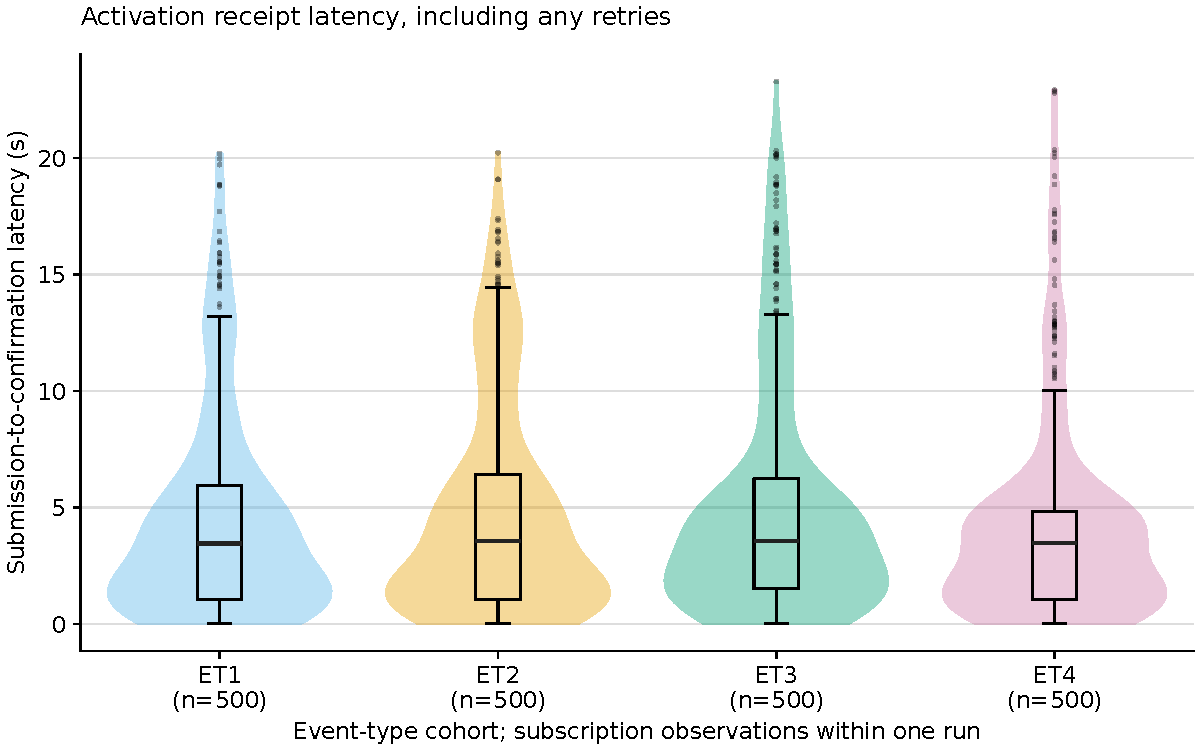
\includegraphics[width=0.92\textwidth]{figures/activation-latency-violin-box.pdf}
  \caption{Within-run activation latency $\ell_k^{\mathrm{act}}=t_k^{\mathrm{ready}}-t_k^{\mathrm{send}}$ for 500 subscriptions
  in each event-type cohort. Violin widths show smoothed empirical density;
  boxes show the interquartile range and median. Whiskers use 1.5 interquartile
  ranges, with observations beyond them retained as points. These are
  subscription observations in one run, not independent cluster trials.}
  \Description{Four violin and box plots show activation receipt latencies.
  Medians are approximately three and a half seconds, with observed upper
  tails reaching roughly twenty to twenty-three seconds.}
  \label{fig:mumbai-activation-latency}
\end{figure}
\FloatBarrier

Figure~\ref{fig:mumbai-activation-latency} distinguishes an individual request's
latency from the time to activate the complete population. Cohort medians were
3.443, 3.560, 3.567 and 3.476 seconds; nearest-rank 99th percentiles were
18.805, 16.907, 20.072 and 20.038 seconds. The subscriptions share upstream services and scheduling conditions, so their
observations are dependent. The distributions describe within-run variation,
without estimating a between-policy confidence interval. A concurrent
thread snapshot found fourteen subscription handlers waiting for upstream
transition confirmation. This locates the observed startup bottleneck in
upstream confirmation waits; the snapshot does not establish CPU saturation.

The complete ledger covers observed delivery attempts, with publisher-to-Queue
event counts outside its scope. This qualification establishes
receipt-confirmed activation under delivery load, probe-based redistribution
with a 60\% reduction in source subscriptions, and reconciled closure. The
recorded delivery rates include workload depletion and startup, so the
experiment reports redistribution rather than an isolated throughput effect.

\subsection{Loaded DQL Migration During Pod Scale-Out}
\label{sec:live-dql-scaleout}

We next tested selective connection replacement during event delivery in a
separate Oracle Cloud cluster run. One client attached 1,000 registered
subscriptions to four persistent connections on one subscriber Pod, with
250 subscriptions per connection. The isolated deployment then grew from
one to four Ready Pods while the same client process remained running.
The second Pod became Ready before standby activation was released; the
third and fourth Pods were added during observation. The transport load
balancer assigned each empty probe to a Pod. The client used the retained
socket only when DQL selected migration and the execution guards passed.

The frozen checkpoint had 9,985 training updates and used $\epsilon=0$.
The trial allowed three executed actions in a configured 600-second window,
with a 60-attempt probe-discovery budget. Telemetry had to satisfy the
180-second age limit and 0.8 minimum backlog coverage. Each Pod requested
1.5 CPU cores and 4~GiB memory, with limits of three cores and 6~GiB.
The client used 32 workers and a fixed one-second processing delay to keep
work outstanding during handoff. This setting tests acknowledgement-aware
migration under a bounded client drain rate, rather than maximum Pod capacity.

Two bounded batches each published four synthetic source events. Each event
matched 5,000 registered subscriptions, including the client's 1,000-subscription
cohort. Thus, publication exposed the queue to 40,000 copies while the measured
cohort accounted for 8,000 delivery attempts. Capacity was checked before each
batch against the existing 400~MB limit, retaining an 80~MB reserve and prior
unreconciled publication costs. No queue purge or quota increase was used.

\begin{table}[!htbp]
  \centering
  \small
  \caption{Executed frozen-DQL handoffs in the loaded Oracle Cloud scale-out
  run. P1 is the initial Pod; P2 and P3 are added Pods. Drain time is included
  in total handoff time. These are three actions within one run.}
  \Description{Three handoffs each move 250 subscriptions and retain the other
  three active sessions. The first two move from P1 to P2; the third moves the
  first group again from P2 to P3. Total times are 97.555, 10.881 and 79.657 seconds.}
  \label{tab:live-dql-loaded-handoffs}
  \begin{tabular}{llrrrr}
    \toprule
    Action & Path & Subscriptions & Other sessions & Drain (s) & Total (s) \\
    \midrule
    H1 & P1 to P2 & 250 & 3 retained & 93.862 & 97.555 \\
    H2 & P1 to P2 & 250 & 3 retained & 8.339 & 10.881 \\
    H3 & P2 to P3 & 250 & 3 retained & 76.166 & 79.657 \\
    \bottomrule
  \end{tabular}
\end{table}

Table~\ref{tab:live-dql-loaded-handoffs} records actual policy execution, not
just a migration recommendation. The three observed differences between the
migration and stay Q-values were 1.7126, 1.2919 and 1.8201. Each migration was
admissible and selected by the frozen network. Before-and-after session maps
show that every handoff preserved the other three active connections. Two
original sessions remained unchanged throughout the run. The mechanism
therefore replaced selected connections without disconnecting the whole pool.

\begin{figure}[!htbp]
  \centering
  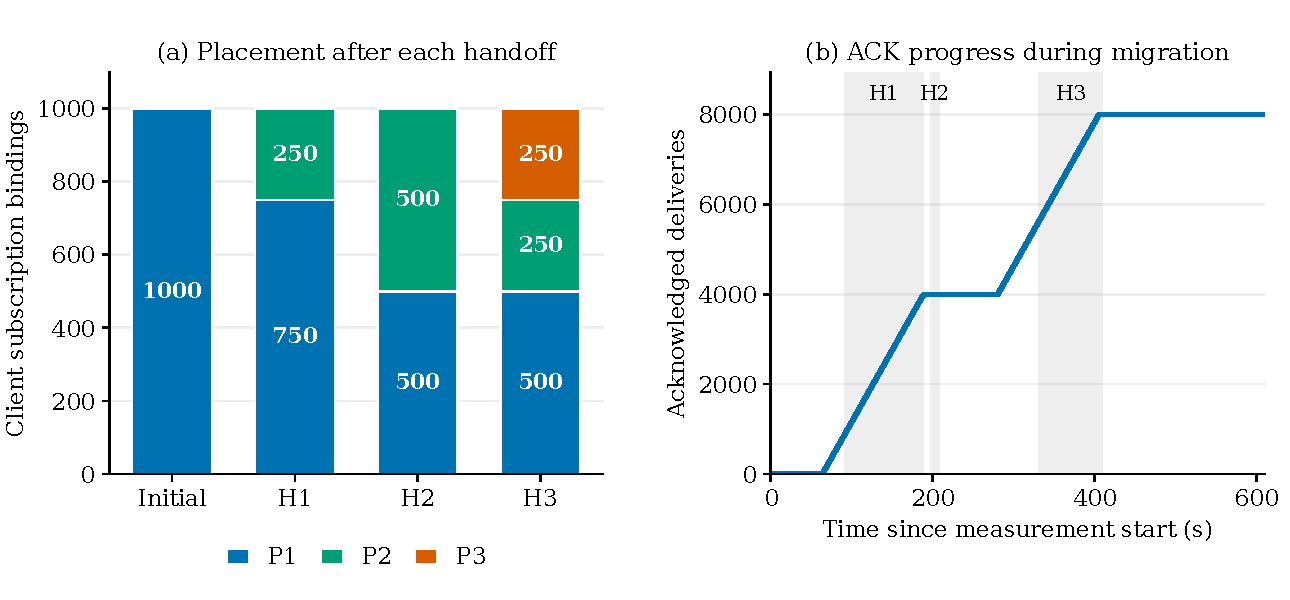
\includegraphics[width=\textwidth]{figures/live-dql-loaded-scaleout.pdf}
  \caption{Measured loaded DQL migration in the Oracle Cloud cluster.
  (a) Receipt-confirmed client bindings at the initial snapshot and after
  H1--H3. Each bar accounts for all 1,000 subscriptions; the four active
  connections each retain 250 subscriptions. P4 has no client bindings and
  is observed only through a probe. (b) Cumulative ACK receipts, aggregated
  in one-second bins. Shaded spans show the measured complete handoff
  intervals, including source drain. The curve describes this bounded
  workload, not a matched between-policy throughput comparison.}
  \Description{Placement changes from one thousand bindings on P1 to seven
  hundred fifty on P1 and two hundred fifty on P2, then five hundred on each,
  and finally five hundred on P1, two hundred fifty on P2 and two hundred fifty
  on P3. ACK receipts reach eight thousand while three shaded handoff intervals
  mark selective connection migration.}
  \label{fig:live-dql-loaded-scaleout}
\end{figure}

Figure~\ref{fig:live-dql-loaded-scaleout}(a) separates moved subscriptions
from handoff operations. H3 moves the group already transferred by H1, so
the three actions comprise 750 subscription-handoff operations involving
500 distinct subscriptions. The final distribution across the four available
Pods is 500, 250, 250 and zero. The maximum client population on one Pod falls
from 1,000 to 500, a 50\% reduction, without increasing the four active
connections. The last Pod remains a probe candidate after the three-action
budget is reached. Discovering it does not automatically promote it.

Figure~\ref{fig:live-dql-loaded-scaleout}(b) uses the confirmed ACK receipt
timestamp of each recorded delivery. Its cumulative total reaches 8,000,
and each of the 1,000 registered subscription hashes has eight acknowledged
delivery records. The ledger contains zero recorded ACK failures, processing
failures, duplicate candidates or unresolved deliveries at clean closure.
Long drain intervals remain visible: source retirement waits for outstanding
work instead of discarding it to shorten the measured handoff. The configured
window contains 60 decision records; its actual measurement boundaries span
609.716 seconds, including boundary handling.

The identity check uses STOMP message identifiers and confirms observed
delivery/ACK accounting. Source CloudEvent identities and individual backend
queue deletions are outside that ledger's scope. A separate unloaded
1,000-subscription run executed two handoffs in 5.244 and 5.172 seconds;
those timings are retained separately because the processing conditions
differ. The online and target weights remained identical to the input
checkpoint in both runs. The loaded run saved 39 valid experience transitions
without applying new training updates. The complete private archive verifies
256 files, and the manuscript figure uses identifier-free aggregates derived
from those records. The isolated deployment was restored to one Ready Pod;
all 13 shared-resource isolation checks passed.

\FloatBarrier

\subsection{TTL-Based Reconnection Under Delivery Load}
\label{sec:ttl-reconnection}

Time-to-live (TTL) reconnection is an existing alternative to client-directed
connection replacement in the subscriber service. It was disabled in the
preceding Oracle Cloud cluster experiments and enabled in the isolated
recovery trials reported below. The deployment
team reported that enabling age-based disconnection under event load caused
widespread delivery interruptions and slow resubscription: delivery restarted
on early-restored subscriptions while the remaining subscriptions were still
being attached. These operational reports provide context rather than a
frequency or severity estimate. The matched-preload trial in
Section~\ref{sec:ttl-preload-results} measures
expiry-related interruptions and ACK completion using server-correlated records.

\subsubsection{Implemented Expiry and Recovery Paths}

The server enables expiry only when the configured connection TTL is positive.
For a connection established at time $t_c^{\mathrm{open}}$, its nominal expiry is
\[
 t_c^{\mathrm{exp}}=t_c^{\mathrm{open}}+T_{\mathrm{TTL}}+60J_c,
 \qquad J_c\in\{1,\ldots,60\},
\]
where $T_{\mathrm{TTL}}$ is in seconds and $J_c$ is the implementation's
uniformly sampled integer jitter in minutes. A scheduled scan runs with a
60-second fixed delay. An expired connection is submitted to a cleanup
executor, its server-side subscription associations are removed, and its
socket is closed. Scheduling and cleanup add delay beyond $t_c^{\mathrm{exp}}$; the scan
interval is not a hard upper bound on closure latency. Several expired
connections can be selected in one scan, although the random jitter reduces
deliberate synchronization. The implementation does not imply that every
client connection expires simultaneously.

The Python client reconnects the affected socket through the transport load
balancer and resends the subscriptions retained for that socket. Recovery applies to the affected connection. It does not automatically
restart the whole client pool. Each
subscription retains its previous delivery state. Consequently, an active
subscription requests active delivery immediately on resubscription; there is
no whole-connection barrier that first restores every subscription and then
releases their events together. Transport reconnection can therefore finish
well before subscription restoration.

This sequence explains the two distinct concerns in the operational report.
First, the expired socket cannot deliver while it is being replaced, and
overlapping recovery intervals can interrupt a large fraction of the pool.
Second, early-restored subscriptions can resume event delivery while other
\texttt{SUBSCRIBE} operations are still outstanding. Delivery and restoration
then overlap in the same service. The server's cleanup also traverses shared
subscription state under a write lock. These operations can compete for shared resources. Their effects on throughput
and latency depend on workload and cannot be inferred from connection age alone.

\begin{table}[!htbp]
  \centering
  \small
  \renewcommand{\arraystretch}{1.18}
  \caption{Implemented TTL reconnection versus guarded DQL migration.
  This compares control mechanisms, not measured performance rankings.}
  \Description{TTL selects connections by age, closes them and reconnects through
  the load balancer. DQL evaluates a retained probe, establishes standby bindings,
  drains the source and activates the replacement before retiring the old socket.}
  \label{tab:ttl-mechanism-comparison}
  \begin{tabular}{p{0.20\linewidth}p{0.34\linewidth}p{0.34\linewidth}}
    \toprule
    Property & Existing TTL strategy & Guarded DQL migration \\
    \midrule
    Trigger & Age, jitter and periodic scan & Observed pressure, Q-values and feasibility guards \\
    Destination & Reconnect assigned by load balancer & Existing load-balancer-assigned probe evaluated before promotion \\
    Replacement & Cleanup and close before reconnect & Target standby before source quiescence and drain \\
    Subscription restart & Retained active subscriptions resume individually & Receipt-gated handoff and controlled target activation \\
    In-flight work & No DQL drain barrier in TTL closure path & Source drain checked before retirement \\
    Scope & Every connection eligible by expiry time & Bounded selected connection; other sockets retained \\
    \bottomrule
  \end{tabular}
\end{table}
\FloatBarrier

Table~\ref{tab:ttl-mechanism-comparison} identifies the intended advantage of
probe-guided migration: destination evaluation and subscription handoff happen
before the old socket is retired. TTL can also reach a newly added Pod, but
selects by connection age rather than the destination's subscription or backlog
pressure. DQL evaluates that pressure and controls source retirement; its
handoff duration still includes source drain and target activation, so delivery
can pause during the transfer.

\subsubsection{Recovery Endpoints and Verification}

Let $d_c$ be the observed disconnect time, $h_c$ the replacement
\texttt{CONNECTED} time, and $r_c$ the time when all retained subscriptions
have successful replacement-session receipts. The two recovery endpoints are
\[
 T_c^{\mathrm{conn}}=h_c-d_c, \qquad T_c^{\mathrm{restore}}=r_c-d_c.
\]
If recovery is incomplete at the next disconnect or the end of observation,
we record only the elapsed waiting time. This is a right-censored observation,
not a successful fast reconnect. Let $s$ denote elapsed trial time in seconds,
and let $I_c(s)$
equal one while connection $c$ is disconnected or its retained bindings remain
unrestored, and zero otherwise. With $\mathcal{C}_0$ denoting the active
connection pool at the start of a TTL trial, the affected fraction is
\[
 F(s)=\frac{1}{|\mathcal{C}_0|}
 \sum_{c\in\mathcal{C}_0} I_c(s).
\]
The peak of $F$ and its time integral distinguish a brief single-socket outage
from widespread or prolonged recovery. Delivery-rate degradation on sockets
that remain connected is measured separately; it is not counted as a physical
disconnect. We also measure unique receipt-confirmed ACK rate, gaps between deliveries,
pending subscription count, and receipt latency per subscription. These show
the effects on both event delivery and subscription operations. Events delivered before $r_c$
directly establish overlap between delivery and incomplete restoration, but
overlap alone does not prove CPU or network saturation.

The recovery instrumentation requests receipts for reconnect subscriptions
without serializing their dispatch. It preserves pending caller Futures,
distinguishes successive sessions, and stores timestamps alongside the exact
delivery ledger. A common instrumentation contract defines the measurements
across comparison arms.
Client disconnects are attributed to TTL only when matched to server expiry
records; unrelated network failures remain separate.

The implementation-level checks exercise the disabled TTL branch, expired
connection closure, and selection of expired rather than unexpired sockets
in a common scan. Client checks cover receipt ownership, unchanged delivery
states, interrupted recovery, and censored timing analysis. These checks
validate implementation behavior. The live comparisons reported below measure
expiry-related interruptions, receipt completion, and recovery timing using
the native jitter. This separates observed behavior from an artificial
simultaneous-disconnection scenario.

\subsubsection{Recovery Observed Within the Existing Storage Limit}

The isolated recovery trial retained the installed 400,000,000-byte Queue
limit and consumed existing experimental events without a storage increase
or new publication. Four clients attached 1,250 subscriptions each to one
subscriber Pod, giving 5,000 receipt-confirmed standby subscriptions across
20 delivery connections and four probes. Each delivery connection held 250
subscriptions. Activation then released delivery with a bounded window of
16 outstanding requests per client. Native TTL used a configured value of
60 seconds with the original 1--60-minute jitter and scheduled scan; no
simultaneous-disconnection rule was introduced.

A sealed client record captures a complete recovery of 250 retained
subscriptions. The replacement socket reached \texttt{CONNECTED} in
0.018 seconds, whereas receipt-confirmed restoration took 104.174 seconds.
During that restoration interval, 82 delivery attempts arrived on the
replacement session. Thus, transport recovery did not mean that the
subscription population was ready, and delivery demonstrably overlapped
with restoration. The corresponding server expiry record was not retained. We therefore report
this as recovery during a TTL-enabled trial, not as a disconnect independently
confirmed to have been caused by TTL. A second client record does match an
explicit server TTL-close request by session identity and records the
subsequent disconnect; this partial run confirms that native expiry occurred, but it is not a
completed performance trial.

The TTL-enabled execution ended during activation after a receipt timeout.
One client sealed its evidence; the supervisor's earlier cleanup deadline
interrupted the other three before sealing. These records are retained as
diagnostics rather than treated as four successful repetitions. ACK errors
also occurred on connections without a recorded disconnect, so they are not
all assigned to TTL. The observed recovery sequence supports distinguishing
socket readiness, subscription readiness and delivery activity; it does not
by itself estimate a TTL-versus-DQL throughput effect.

After restoring TTL to its disabled state, a functional control used the same
5,000-subscription population and existing events. Its four verified client
records contain 117,269 delivery attempts, 110,411 receipt-confirmed ACKs and
6,858 unresolved attempts. No active-connection interruption was recorded,
but activation ended after an explicit upstream state-transition failure
exhausted its retry budget; 2,929 bindings had confirmed active state in the
last progress records. This distinguishes the expiry/recovery mechanism from
an activation bottleneck that also occurs without TTL. Because the first
execution had already consumed part of the workload, the two runs do not
provide a matched-backlog throughput comparison. Both preserve the frozen
model without additional training. The isolated Deployment was restored,
and all thirteen shared-resource isolation checks passed.

% Live measurements only. Derived figures and aggregates retain the sealed
% September 25 evidence hashes; simulator results are not pooled with this pair.
\subsubsection{Native TTL During Two Delivery Bursts}
\label{sec:ttl-loaded-results}

Before the preload trial, a separate live pair tested native TTL against a
static TTL-disabled control on one isolated Oracle Cloud subscriber Pod.
Both arms used 5,000 subscriptions, five clients, 20 occupied connections and
five empty probes, with zero artificial client processing delay. Each started
from an empty Queue and received two bursts of three accepted source events,
giving 30,000 recorded delivery attempts per arm. Both used the same server
image and 900-second post-activation observation. Native TTL retained its
original jitter. The control replayed the accepted burst schedule: its first
requests were 0.462 and 0.578 seconds later than the native relative targets
of 26.182 and 319.207 seconds. Queue-statistics budget failures stopped other
publication blocks before any event attempt; those failures were retained.

\begin{table}[!htbp]
 \centering
 \small
 \renewcommand{\arraystretch}{1.14}
 \caption{Oracle Cloud two-burst TTL comparison, separate from the subsequent
 preload pair. Both arms use static placement on one Pod; TTL off is not a
 learned DQL intervention. Latency statistics include confirmed ACKs only.}
 \Description{Native TTL records five interruptions, 369 unresolved receipts
 and a 238.392-second confirmed ACK latency p95. The static TTL-disabled control
 records zero interruptions, no unresolved receipts and a 55.826-second p95.}
 \label{tab:ttl-loaded-results}
 \begin{tabular}{p{0.51\linewidth}rr}
  \toprule
  Measurement & Native TTL & Static TTL off \\
  \midrule
  Delivery attempts & 30,000 & 30,000 \\
  Receipt-confirmed ACKs & 29,631 & 30,000 \\
  Unresolved ACK receipts & 369 & 0 \\
  Server-matched TTL interruptions & 5 & 0 \\
  Confirmed ACK latency: median (s) & 19.439 & 21.407 \\
  Confirmed ACK latency: 95th percentile (s) & 238.392 & 55.826 \\
  Clients with receipt-complete shutdown & 2 of 5 & 5 of 5 \\
  \bottomrule
 \end{tabular}
\end{table}

Table~\ref{tab:ttl-loaded-results} shows the tail that a median alone would
miss: native TTL's confirmed-ACK p95 was 4.27 times the control's, although its
median was 1.968 seconds lower. Five interruptions matched server expiry records.
Transport reconnection took 17--24~ms, whereas restoring all 250 bindings on
each affected connection took 0.504--0.973 seconds. One recovery received
22 delivery callbacks before all binding receipts arrived. This directly
demonstrates delivery overlapping resubscription within the observed short
recovery windows; prolonged stalls and whole-pool expiry were not observed. All 369 unresolved
attempts belonged to expired sessions; three clients reached the 120-second
receipt-drain deadline. Missing receipts are not counted as lost Queue events.
All ten sealed client bundles were recovered and verified. This single
sequential pair measures TTL-related disruption and confirmed-receipt latency
under static placement. It estimates neither repeated-run capacity nor a
DQL-specific effect.

\subsubsection{Matched-Preload Comparison in the Oracle Cloud Cluster}
\label{sec:ttl-preload-results}

A subsequent isolated trial compared native TTL with the frozen DQL controller
under the same initial queued workload. Each arm used the same 5,000 registered
ET1 subscriptions: five clients held 1,000 subscriptions each on four occupied
connections, with 250 subscriptions per connection and one empty probe per
client. All 20 occupied connections initially terminated on one subscriber Pod.
Three identical Pods became Ready before activation. Each Pod had a limit of
three CPU cores and 6~GiB memory, and both arms used the same pinned server image.
The installed Queue limit remained 400,000,000 bytes; shared subscriber
resources were not changed.

All bindings were attached in standby before six source events were published
through the authenticated ingest path. A pre-activation Queue snapshot verified
30,000 visible copies and zero in-flight copies in each arm. The recorded
delivery ledger subsequently contained six attempts for every subscription in
the same 5,000-subscription cohort. Native TTL retained the 60-second base,
1--60-minute random jitter and scheduled scan. The DQL arm disabled TTL and
loaded unchanged online and target networks from the checkpoint with 9,985
training updates; exploration and further learning were disabled. Observation
continued for 900 seconds after activation, with activation itself also recorded.

The original workload included a six-event refill at five minutes. Its first
Queue-statistics budget check returned HTTP~429 before any event was attempted.
Before the DQL arm started, the comparison was amended to use the six-event
preload without refill. Three DQL preload budget checks also failed before
publication; cooldown and fresh checks admitted the remaining events while all
bindings stayed in standby. The initial copy counts therefore matched, but the setup proceeded at
different rates. Queue occupancy was approximately 20.3~MB in both arms, not
400~MB. This sequential pair measures fixed-preload drainage. Sustained
arrivals and subscriber saturation are outside that workload.

\subsubsection{Receipt Completion and Connection Recovery}

Table~\ref{tab:ttl-preload-results} reports the observed outcomes. Let
$D_{\mathrm{obs}}$ be the number of recorded delivery attempts and
$A_{\mathrm{conf}}$ the number with a confirmed ACK receipt. Receipt completion is
$A_{\mathrm{conf}}/D_{\mathrm{obs}}$; the remainder is unresolved, not classified as
event loss. Both arms recorded 30,000 attempts. Native TTL confirmed 26,831 ACKs
(89.44\%), compared with 30,000 (100\%) in the TTL-disabled arm, a difference of
10.56 percentage points in this pair. The latter arm is labelled
\emph{guard-held DQL}: its controller ran, but telemetry guards held every
decision at \emph{stay}, as explained below.

\begin{table}[!htbp]
 \centering
 \small
 \renewcommand{\arraystretch}{1.14}
 \caption{Measured Oracle Cloud outcomes for the matched 5,000-subscription
 preload. The DQL arm had TTL disabled and executed no migration. Latencies
 are conditional on confirmed ACKs; unresolved receipts are reported separately.}
 \Description{Both arms record thirty thousand delivery attempts. Native TTL
 has twelve server-matched interruptions and 3,169 unresolved receipts. The
 guard-held DQL arm has neither, but executes no migrations.}
 \label{tab:ttl-preload-results}
 \begin{tabular}{p{0.49\linewidth}rr}
  \toprule
  Measurement & Native TTL & Guard-held DQL \\
  \midrule
  Delivery attempts & 30,000 & 30,000 \\
  Receipt-confirmed ACKs & 26,831 & 30,000 \\
  Unresolved ACK receipts & 3,169 & 0 \\
  Receipt completion (\%) & 89.44 & 100.00 \\
  Server-matched TTL interruptions & 12 & 0 \\
  Distinct occupied sockets interrupted & 11 of 20 & 0 of 20 \\
  Peak simultaneously recovering sockets & 3 of 20 & 0 of 20 \\
  Incomplete-restoration exposure (connection-s) & 10.983 & 0 \\
  Confirmed ACK latency: median (s) & 69.862 & 69.836 \\
  Confirmed ACK latency: 95th percentile (s) & 251.546 & 249.874 \\
  Executed DQL migrations & Not applicable & 0 \\
  \bottomrule
 \end{tabular}
\end{table}

All twelve native interruptions matched server expiry records by session
identity and disconnect time. They affected eleven distinct occupied sockets,
with at most four interrupted within a rolling minute. At most three sockets
were concurrently unrestored, giving $\max_s F(s)=3/20=0.15$ and
$\int\sum_c I_c(s)\,ds=10.983$ connection-seconds. Complete binding
restoration took 0.492--1.835 seconds. These observations show overlapping
recovery periods affecting part of the pool, rather than a whole-pool outage. All 3,169 unresolved native
attempts belonged to sessions with matched expiries, but a missing ACK receipt
does not reveal whether the underlying Queue deletion succeeded.

\begin{figure}[!htbp]
 \centering
 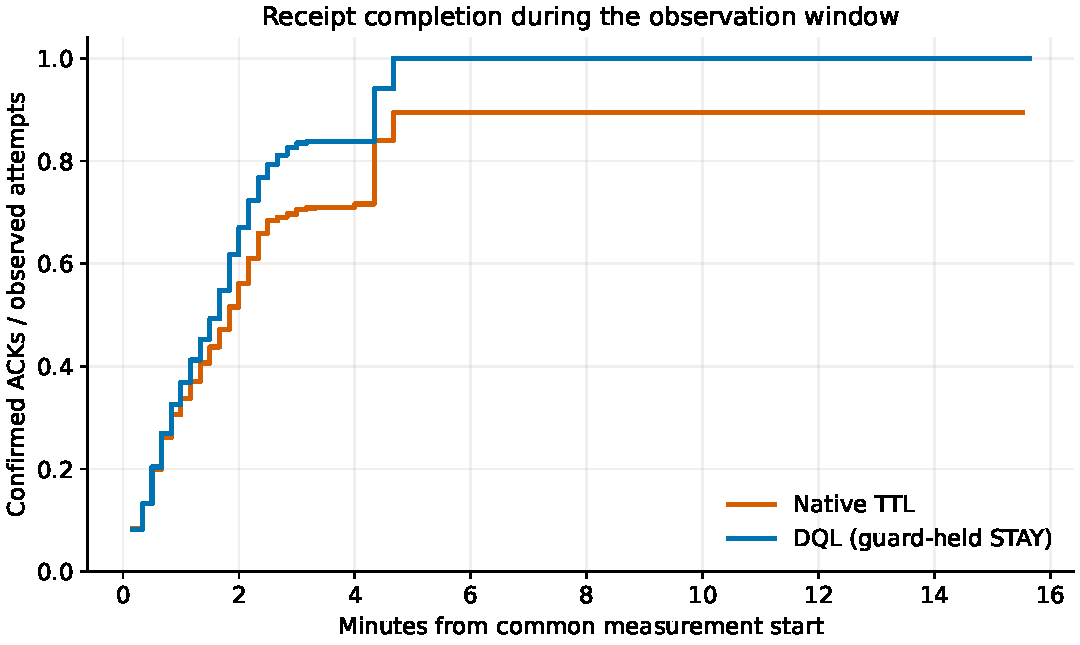
\includegraphics[width=0.88\textwidth]{figures/ttl-preload-ack-completion.pdf}
 \caption{Receipt completion in the Oracle Cloud matched-preload pair.
 Each curve accumulates confirmed ACKs in ten-second bins and divides by all
 30,000 observed attempts in its arm. Unresolved attempts remain in the
 denominator. DQL denotes the guard-held, TTL-disabled execution, not a
 completed migration comparison.}
 \Description{Native TTL receipt completion reaches 89.44 percent and the
 guard-held DQL arm reaches 100 percent. The horizontal axis is minutes from
 the common measurement start within each arm.}
 \label{fig:ttl-preload-completion}
\end{figure}

Figure~\ref{fig:ttl-preload-completion} retains the unresolved attempts in the
final level rather than rescaling each curve using only successful attempts.
Time starts when all five client observation windows overlap within each arm. Those common windows lasted 931.347 and 937.743 seconds,
respectively. Their mean confirmed-ACK rates were 28.809 and 31.992/s, including
idle time; these are whole-window completion rates, not estimates of maximum
Pod bandwidth. Four native clients reached the 120-second final ACK-drain
deadline. We retain their incomplete drains and the coordinator's nonzero exit status
as outcomes. All ten client evidence bundles were sealed and verified;
the DQL coordinator completed cleanly.

\begin{figure}[!htbp]
 \centering
 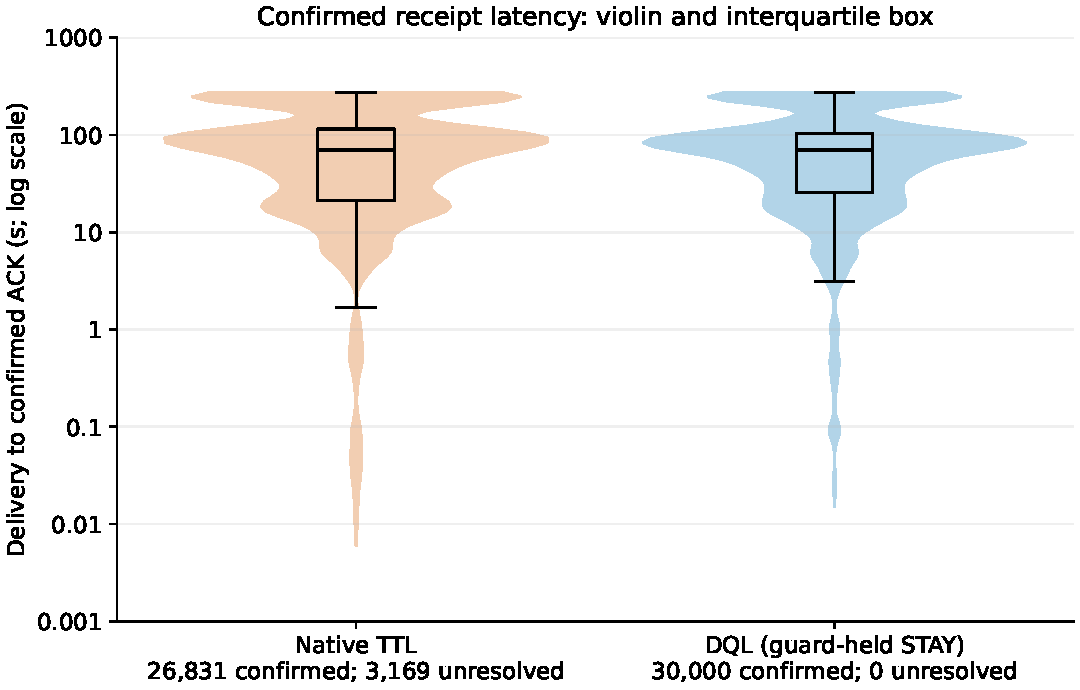
\includegraphics[width=0.88\textwidth]{figures/ttl-preload-ack-latency-violin-box.pdf}
 \caption{Confirmed delivery-to-ACK latency in the Oracle Cloud preload pair.
 Violin density is estimated on $\log_{10}$ latency; boxes show its median and
 interquartile range, with 1.5-IQR whiskers. Outlier markers are suppressed,
 not removed from the observations. Counts exclude unresolved receipts.}
 \Description{Violin and box plots compare 26,831 confirmed native TTL
 latencies with 30,000 guard-held DQL latencies. Their medians are approximately
 seventy seconds. Native TTL additionally has 3,169 unresolved receipts.}
 \label{fig:ttl-preload-latency}
\end{figure}

Figure~\ref{fig:ttl-preload-latency} separates receipt completion from
conditional latency. The confirmed medians differ
by only 0.026 seconds, and the 95th percentiles are also close. Native unresolved
receipts are absent from this latency distribution but remain explicit in
Table~\ref{tab:ttl-preload-results}. Violin width describes within-run latency
variation. The five clients and 30,000 attempts belong to one pair rather than
independent trials, so between-run uncertainty is not estimated. Unlike the
earlier 104.174-second diagnostic, this pair recorded no new delivery callbacks
during subscription-restoration windows. It captures a different recovery
condition from resubscription under concurrent delivery.

\subsubsection{Telemetry Freshness and Action Eligibility}

The DQL trace contains 450 decision intervals, all held at \emph{stay} by
\texttt{invalid-backlog-telemetry}. No migration executed, and all 5,000 bindings
remained on the source Pod despite four Pods being Ready. Statistics collection
paced individual subscription requests at 40~ms for a 5,000-subscription sweep.
Even before network delay or retries, the sweep required at least
$5{,}000\times0.040=200$ seconds, exceeding the 180-second oldest-sample deadline.
The minimum coverage across the Pod and occupied-connection components ranged
from 0.560 to 0.808. Only ten observations met every 80\% coverage threshold;
their oldest constituent samples were 183.127--185.974 seconds old and failed
freshness. A recently received telemetry frame can therefore contain stale
Queue observations. Queue-statistics rate limits further constrained coverage.

This finding separates two operational properties. Native expiry produced
measurable interruptions and receipt uncertainty; the TTL-disabled, guard-held
arm preserved its occupied sockets and completed all observed ACKs. Freshness
checks held migration inactive, so the measured benefit concerns connection
retention and receipt completion, rather than throughput from added Pod
capacity. The checkpoint and guards stayed fixed throughout the trial.
Cleanup verified empty Queue and
dead-letter Queue inventories, restored isolated TTL to zero and one Ready Pod,
and passed all thirteen shared-resource isolation checks.
\FloatBarrier



\section{Experimental Method and Locked Simulator Evidence}
\label{sec:locked-evidence}

We evaluate recovery after subscriber-pod scale-out using 20,000 subscriptions,
ten persistent connections, and 775 million queued events. The primary
comparison measures the use of added pod capacity with guarded-greedy and
DQL-guided migration against retaining the initial connection placement. Supporting studies examine
multi-objective control, action selection, and adverse probe promotion.

\subsection{Recovery After Subscriber-Pod Scale-Out}
\label{sec:scaleout-recovery}

The primary recovery experiment models the capacity increase from one
subscriber pod to four. Ten persistent TCP connections are established on the
original pod, carrying 20,000 subscriptions. At the measurement boundary,
three additional ready pods provide processing capacity, while the ten
established connections retain their original endpoints. The comparison
therefore measures how effectively the client uses the added capacity through
probe promotion and subscription reassociation.

Four equal subscription groups begin with 100,000, 50,000, 5,000, and zero
queued events per subscription, respectively. The initial backlog is
$B(0)=775{,}000{,}000$ events. Round-robin assignment gives each connection
2,000 subscriptions and 77.5 million queued events. Consequently,
$V^N_u(0)=V^G_u(0)=0$: the initial bottleneck is concentrated pod placement.
This setup isolates whole-connection migration from pre-existing imbalance
between the client's connections.

The model assigns each pod a processing threshold of 100,000 events/s and
the client a base acknowledgement capacity of 250,000 events/s. Its bounded
connection-parallelism factor is three at ten connections. Service is limited
by both client capacity and each connection's share of its pod capacity.
The simulator's pressure-dependent service factor is
$\max\{0.35,1-0.42P_i^{\mathrm{sim}}\}$, where $P_i^{\mathrm{sim}}\in[0,1]$ is the simulator's
clipped load score, distinct from the deployable pressure in
(\ref{eq:pod_pressure}). These numerical rates define the simulator's service
assumptions rather than measured Pod benchmarks. Pressure is sampled before the action
and refreshed after the interval. For the clipped score, this service
multiplier lies in $[0.58,1]$: the model represents pressure-degraded service,
not complete Pod service collapse. Arrival rates and processing rates are
converted to event counts using the declared $\Delta=10$ seconds. The drain
phase introduces no new arrivals and lasts 120 intervals, or 20 minutes.

We compare \emph{Frozen DQL}, \emph{Kubernetes scale-out only}, and
\emph{Scripted probe migration}. All three receive the same capacity increase.
The second policy retains the existing connection assignment. The third
promotes every candidate admitted by the migration guard and evaluates the
framework's deterministic guarded-greedy policy. DQL uses the previously frozen checkpoint
without exploration or training. Adaptive policies can replace at most 12
non-improving probes, and actions have a three-interval cooldown.
The scripted control uses no learned Q-values: it shares the pressure-aware
admission rule and source selection with DQL. We therefore distinguish this
\emph{guarded-greedy} policy from the independent ad-hoc schedules below.
Its mean throughput is 221,260 events/s, compared with 219,762 for DQL. These
are two effective selectors for the shared rebalancing mechanism, not evidence
that Q-learning is necessary to use added capacity. The original registered
primary contrast remains DQL versus unchanged placement; this broader
interpretation does not change that protocol or relabel a post-hoc contrast
as confirmatory. An exploratory paired reanalysis of these same twenty seeds
gives a greedy-minus-DQL mean throughput difference of 1,498 events/s
(pointwise percentile bootstrap 95\% interval [362, 2,852], 10,000 resamples).
This small rate advantage belongs to the greedy policy in this workload;
the mixed-workload study evaluates DQL's separate multi-objective benefit.

For remaining backlog $B(t)$, the primary endpoint is the mean normalized
backlog over the recovery window,
\begin{equation}
 \mathrm{AUC}_B=\frac{1}{T}\sum_{t=1}^{T}
 \frac{B(t-1)+B(t)}{2B(0)},\qquad T=120.
 \label{eq:scaleout-backlog-auc}
\end{equation}
Lower $\mathrm{AUC}_B$ indicates less accumulated queued work. Twenty fresh paired seeds
vary probe placement while holding the workload fixed. We use 10,000 paired
bootstrap resamples and 100,000 sign-randomization draws. The registered
criterion requires the upper 95\% confidence bound of the DQL-minus-baseline
AUC difference to be below zero and the one-sided $p$-value to be below 0.05.
These intervals describe variation caused by probe placement within this model.

\begin{table}[!t]
\centering
\small
\caption{Persistent-connection recovery after scaling from one to four subscriber Pods. Twenty paired seeds each start with 20,000 subscriptions and 775 million queued events on ten TCP connections pinned to Pod~0. Lower backlog measures are better.}
\label{tab:persistent_scaleout_recovery}
\resizebox{\linewidth}{!}{%
\begin{tabular}{lrrrrr}
\toprule
Policy & Backlog AUC & Final backlog (\%) & Throughput (k/s) & Active Pods & Migrations \\
\midrule
\textbf{Frozen DQL} & 0.8376 & 65.97 & 219.8 & 4.00 & 7.75 \\
Kubernetes scale-out only & 0.9551 & 91.02 & 58.0 & 1.00 & 0.00 \\
Scripted probe migration & 0.8359 & 65.74 & 221.3 & 4.00 & 7.75 \\
\midrule
\multicolumn{6}{l}{DQL vs. scale-out only: 12.30\% lower backlog AUC; 278.9\% higher mean throughput.} \\
\bottomrule
\end{tabular}
}
\end{table}


Table~\ref{tab:persistent_scaleout_recovery} shows that DQL raises mean
throughput from 58,000 to 219,762 events/s, a factor of 3.79. It reduces backlog
AUC from 0.95510 to 0.83759, an improvement of 12.30\%. The paired AUC
difference is $-0.117504$ (95\% confidence interval
$[-0.121210,-0.113345]$; one-sided $p\simeq10^{-5}$). DQL leaves 65.97\% of
the initial backlog after 20 minutes, compared with 91.02\% for scale-out only,
or 27.52\% less remaining backlog relative to that baseline. All 20 DQL
episodes use all four pods by the end, with a mean of 7.75 connection
migrations. The baseline retains all ten connections on the original pod.

\begin{figure}[!htbp]
 \centering
 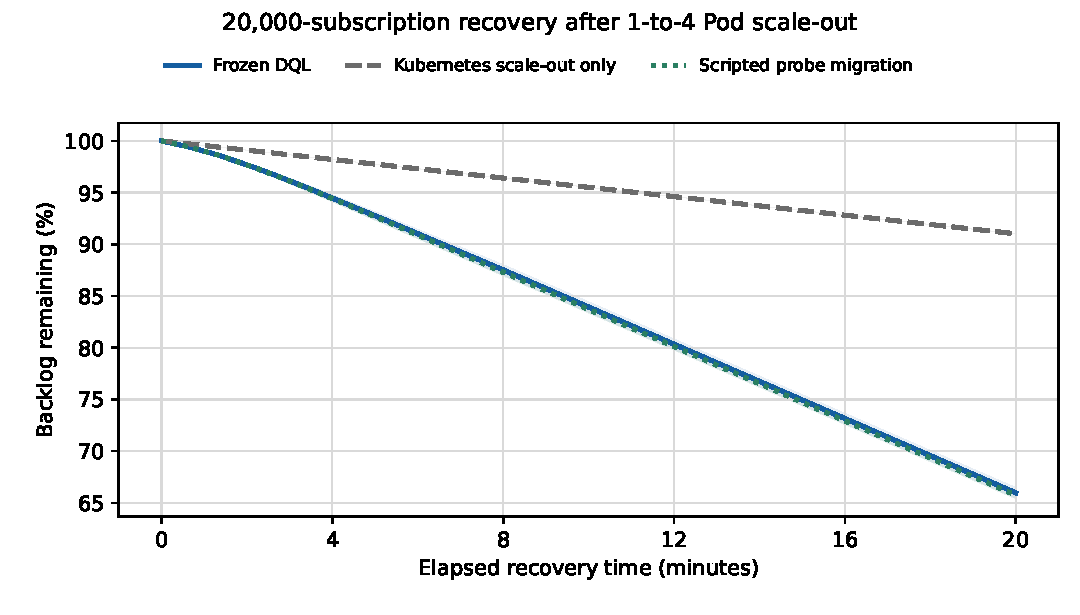
\includegraphics[width=\textwidth]{evidence/persistent-scaleout-recovery-complete/persistent_scaleout_backlog_recovery.pdf}
 \caption{Backlog recovery after adding three subscriber pods. All policies
 start with the same 775-million-event backlog. Curves are means over 20
 paired seeds; shaded bands are descriptive 95\% normal-approximation
 intervals. The area under each normalized curve defines the primary endpoint.}
 \Description{A line chart compares remaining backlog over twenty minutes.
 DQL and scripted probe migration drain substantially more backlog than
 Kubernetes scale-out with the original TCP connection placement.}
 \label{fig:scaleout-backlog-recovery}
\end{figure}

Figure~\ref{fig:scaleout-backlog-recovery} connects the endpoint to the
recovery process. The steeper DQL curve follows successful probe promotions
that place delivery work on additional pods. The nearby scripted-control curve shows that DQL reaches about the same
service capacity as guarded scripted migration. Both improve on the unchanged
placement, establishing the benefit of migration in this workload rather than
a ranking above every controller with the same actions.

\begin{figure}[!htbp]
 \centering
 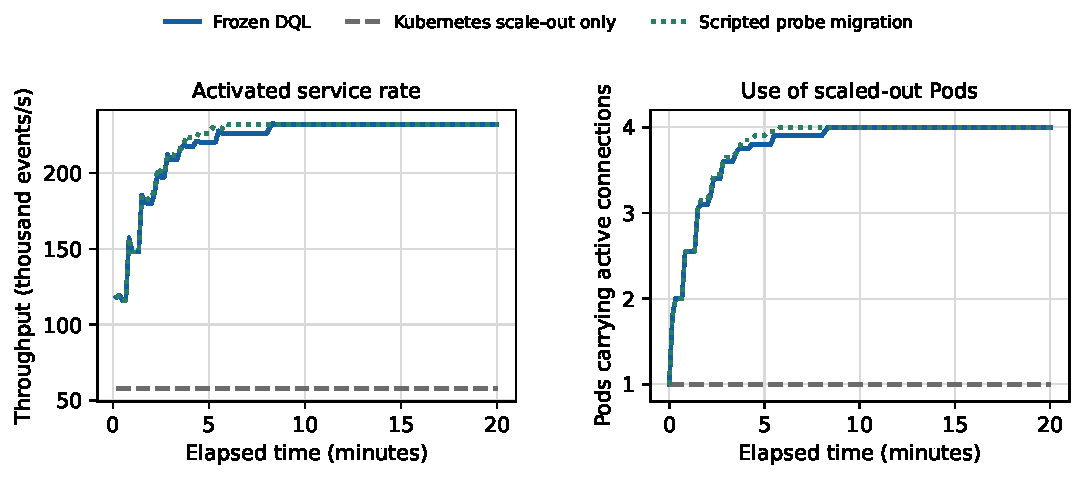
\includegraphics[width=\textwidth]{evidence/persistent-scaleout-recovery-complete/persistent_scaleout_capacity_activation.pdf}
 \caption{Use of the added subscriber capacity. Left: mean delivered events
 per second over each measured interval. Right: mean number of pods carrying
 active client connections. The ten delivery connections are retained as a
 bounded pool while probe promotion replaces their endpoint assignments.}
 \Description{Two line charts show throughput rising as DQL spreads active
 connections across four subscriber pods. The scale-out-only baseline remains
 at one active pod and approximately fifty-eight thousand events per second.}
 \label{fig:scaleout-capacity-activation}
\end{figure}

Figure~\ref{fig:scaleout-capacity-activation} provides the mechanism evidence:
the throughput increase occurs as more pods acquire subscription-bearing
connections. Added pod capacity and client-directed reassociation jointly
produce the gain. In the model's saturated regime, a single pod supplies
approximately 58,000 events/s; four utilized pods supply approximately
232,000 events/s. The mean over the full recovery period is lower because probe discovery
and cooldown take up part of the observation window. The maximum relative difference in queue accounting is $1.45\times10^{-13}$ across the
60 episodes. The simulator represents reassociation as a discrete action;
network delays and the live receipt protocol are outside this timing model.

Figure~\ref{fig:scaleout-violin-distributions} makes the seed-to-seed
variation behind the recovery averages visible. Each AUC observation is the
episode-level quantity in Eq.~\eqref{eq:scaleout-backlog-auc}; each throughput
observation is the episode's delivered-event total divided by its 1,200-second
duration. The violin uses a Gaussian kernel with Scott's bandwidth,
$h=s_{\mathrm{sample}} n_{\mathrm{ep}}^{-1/5}$ for sample standard deviation $s_{\mathrm{sample}}$ and $n_{\mathrm{ep}}=20$, and is drawn only
between the smallest and largest observations. Its width is descriptive, not
a confidence interval. The scale-out-only outcomes are constant because that
policy never changes its initial placement. The adaptive distributions reflect
variation in probe discovery and migration timing. Their separation from the baseline agrees with the paired AUC result above.
The overlapping DQL and scripted distributions describe similar recovery
performance for these two policies, without establishing DQL superiority over
the guarded scripted control.

\begin{figure}[!htbp]
 \centering
 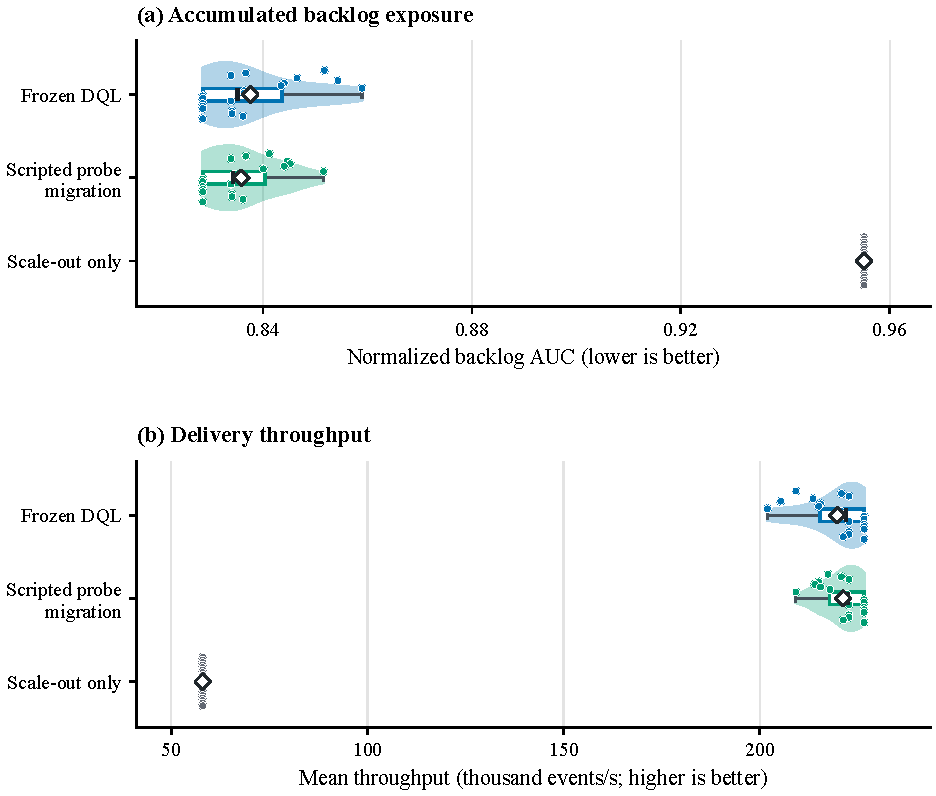
\includegraphics[width=\textwidth]{figures/scaleout-violin-distributions.pdf}
 \caption{Scale-out recovery distributions over 20 paired seeds per policy.
 Violin width shows a kernel-density estimate within the observed range;
 boxes show quartiles and medians, diamonds show means, and points show all
 episodes. Whiskers use the 1.5-interquartile-range rule. The constant
 scale-out-only baseline is shown without an artificial density. Lower
 normalized backlog AUC and higher throughput are preferred.}
 \Description{Two horizontal violin-and-box panels show normalized backlog
 AUC and mean throughput. Frozen DQL and scripted probe migration have lower
 backlog exposure and higher throughput than scale-out alone. Every seed is
 visible; the unchanged-placement baseline has identical values across seeds.}
 \label{fig:scaleout-violin-distributions}
\end{figure}

\paragraph{Independent ad-hoc migration.}
An exploratory extension retains all sixty original observations and adds
eighty episodes: four pressure-unaware schedules evaluated on the same twenty
paired seeds. Each attempt chooses a connection and target Pod uniformly,
without consulting backlog, pressure, or the learned policy. A same-Pod draw
remains a no-op. The schedules use fixed periods of 40 or 60 seconds, or a
60-second nominal period with $\pm30\%$ or $\pm40\%$ uniform timing jitter.
All schedules first act at interval zero. The nominal jitter ranges are
42--78 and 36--84 seconds; rounding upward to the ten-second decision clock
gives executable ranges of 50--80 and 40--90 seconds, respectively. These
percentages modify the schedule, not the measured throughput. Rounding also
changes the average attempt frequency, so jitter is not isolated from timing.
In the following comparison, \emph{Scripted} denotes the independent
60-second schedule with $\pm30\%$ timing jitter; \emph{guarded-greedy migration}
denotes the original pressure-aware positive control. These are distinct
non-learning policies.

\begin{table}[!htbp]
\centering\small
\caption{Independent ad-hoc migration sensitivity in the scale-out simulator. Means over twenty paired seeds per policy; timing jitter changes the schedule, not measured values.}
\label{tab:adhoc-migration}
\begin{tabular}{lrrrr}
\toprule
Policy & Events/s & Backlog AUC & Migrations & Final Pods \\
\midrule
Frozen DQL & 219,762 & 0.83759 & 7.75 & 4.00 \\
Guarded-greedy migration & 221,260 & 0.83589 & 7.75 & 4.00 \\
Ad-hoc: fixed 40 s & 205,295 & 0.84997 & 22.85 & 3.70 \\
Ad-hoc: fixed 60 s & 197,636 & 0.85906 & 15.40 & 3.90 \\
Scripted & 195,737 & 0.86064 & 14.70 & 3.85 \\
Ad-hoc: 60 s, $\pm$40\% & 195,640 & 0.86053 & 14.65 & 3.85 \\
Scale-out only & 58,000 & 0.95510 & 0.00 & 1.00 \\
\bottomrule
\end{tabular}
\end{table}


Table~\ref{tab:adhoc-migration} shows mean DQL throughput of 219,762 events/s,
compared with 195,737 for the $\pm30\%$ schedule and 195,640 for the $\pm40\%$
schedule. The relative gains are 12.27\% and 12.33\%, with pointwise paired
95\% bootstrap intervals of [9.38\%, 15.55\%] and [9.31\%, 15.81\%],
respectively. Each interval uses 10,000 resamples of complete seed pairs and
the ratio of resampled mean rates. DQL uses 7.75 migrations per episode,
compared with 14.70 and 14.65 for the two jittered schedules. The fixed
40-second and 60-second schedules yield gains of 7.05\% and 11.20\%, so the
comparison covers both fixed and jittered schedules. This exploratory
sensitivity analysis reuses the scenario seeds. Its scope is simulated
migration scheduling, separate from independent holdout testing and live
connection-TTL measurements.

\begin{figure}[!htbp]
 \centering
 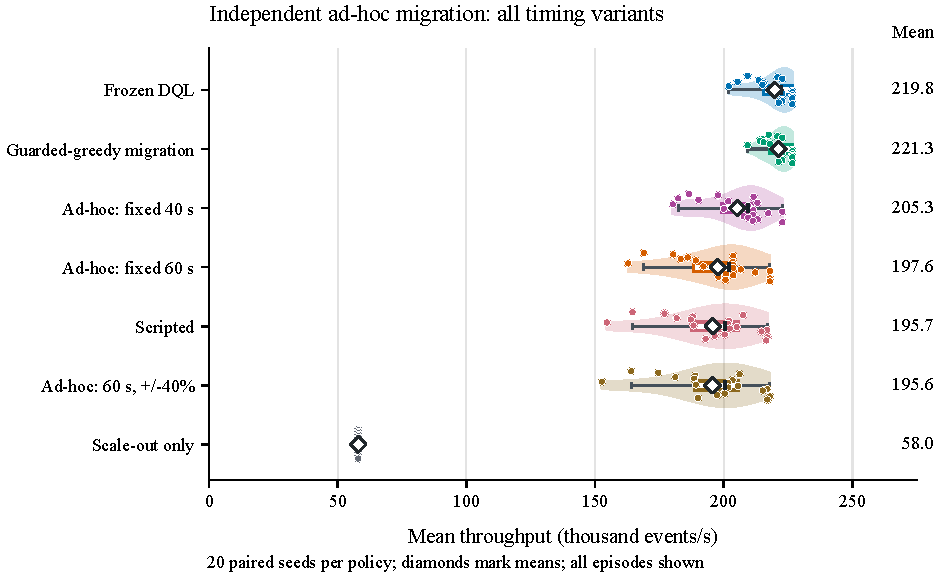
\includegraphics[width=\textwidth]{figures/adhoc-migration-distributions.pdf}
 \caption{Throughput under independent ad-hoc migration schedules. All twenty
 episodes per policy are shown. Violin density uses Scott's bandwidth within
 the observed range; boxes show quartiles and medians, whiskers use the
 1.5-interquartile-range rule, and diamonds mark means. The constant
 scale-out-only control has no artificial density. All seven policies are
 retained, including the original guarded-greedy control.}
 \Description{Seven horizontal violin-and-box rows compare measured simulator
 throughput. DQL has higher mean throughput than every random-endpoint schedule;
 the pressure-aware guarded-greedy control remains close to DQL.}
 \label{fig:adhoc-migration-distributions}
\end{figure}

Figure~\ref{fig:adhoc-migration-distributions} shows the variation hidden by
the averages. Random reassignment can revisit an already occupied Pod or move
work away from a useful placement, whereas the guarded DQL controller admits
pressure-improving candidates. The distributions and migration counts compare
the complete controllers, including their admission and endpoint-selection
rules. The nearby guarded-greedy distribution shows that the result compares
complete policies, including their guards, rather than isolating the effect
of learned action selection.

Figure~\ref{fig:stress-throughput-radar} summarizes the same stressed workload,
rather than importing the mixed-workload radar's averages. Its throughput
coordinate divides each episode's mean rate by the four Pods' combined
nominal capacity, $4\times100{,}000=400{,}000$ events/s. The other coordinates
are the fraction of initial backlog removed, the final active-Pod count
divided by four, and $10/(10+M^{\mathrm{ep}})$ for an episode with $M^{\mathrm{ep}}$ migrations. The last
coordinate decreases with intervention count; it is not a handoff-latency
measurement. Each plotted point averages these per-episode coordinates across
all twenty seeds. No observed-best or policy-specific denominator is used.
The $\pm30\%$ ad-hoc schedule appears alongside the original three controls;
all timing variants remain in Table~\ref{tab:adhoc-migration}.

\begin{figure}[!htbp]
 \centering
 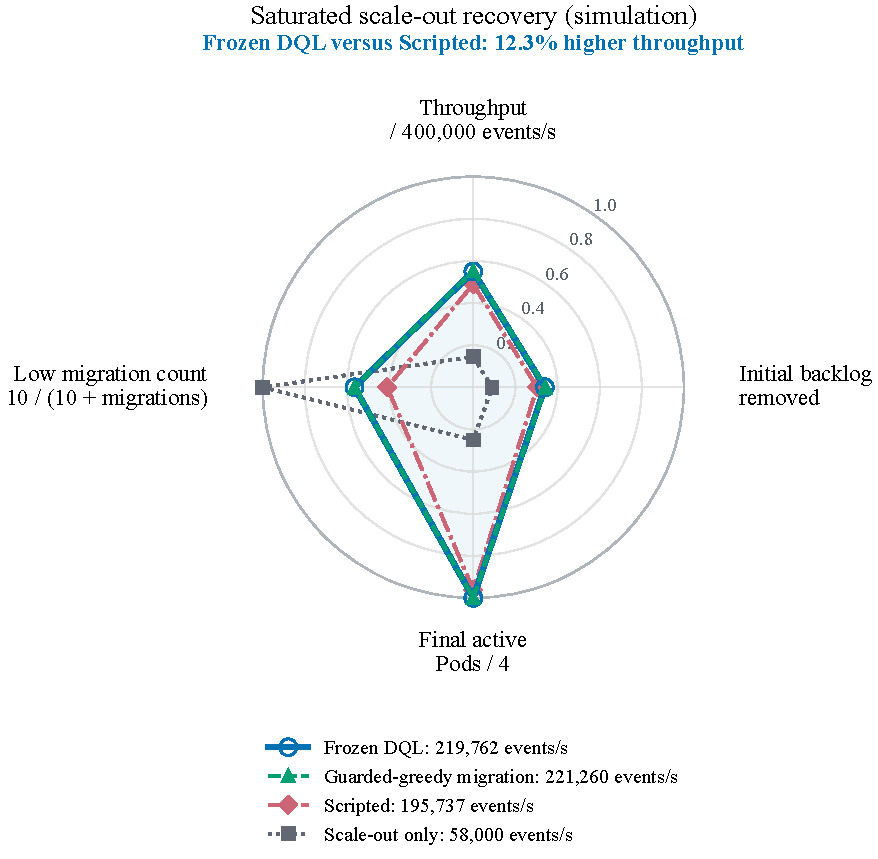
\includegraphics[width=\textwidth]{figures/adhoc-migration-radar.pdf}
 \caption{Stress-scenario radar from all twenty paired simulator seeds per
 displayed policy. \textbf{Frozen DQL versus Scripted: 12.3\% higher throughput},
 with measured mean rates of 219,762 and 195,737 events/s, respectively.
 The guarded-greedy and scale-out-only controls remain visible at 221,260 and
 58,000 events/s. All coordinates use fixed zero-to-one scales, with outward preferred;
 migration count exposes the intervention tradeoff. This is a descriptive
 profile, not an additional objective or statistical test.}
 \Description{A four-axis radar explicitly labels Frozen DQL versus Scripted
 with 12.3 percent higher throughput for DQL.
 It also retains the pressure-aware guarded-greedy and scale-out-only controls,
 and identifies the plotted results as simulator measurements.}
 \label{fig:stress-throughput-radar}
\end{figure}

The DQL throughput radius is 12.3\% larger than the Scripted radius and 3.79 times
the scale-out-only radius because all use the same capacity denominator.
The guarded-greedy comparator has a nearly overlapping profile and slightly
higher mean throughput. The result establishes the benefit of reaching added
capacity, with similar performance from a pressure-aware non-learning control.
Backlog removal and throughput are linked because the workload has no new
arrivals during drainage. They are not independent confirmations. The polygon's
area is not a performance measure. These measurements remain distinct from the Oracle Cloud
expiry and receipt-completion results in Section~\ref{sec:ttl-preload-results}.
\FloatBarrier


\subsection{Supporting Study Design}

The independent v3 holdout compares a frozen DQL policy with deterministic
controls. The adverse-probe ablation holds that checkpoint fixed and varies
the promotion guard, using separate 30-seed inference and five-seed scale
cohorts. Expanded v4--v6 studies evaluate action coverage and contract changes;
they are development diagnostics, not additional holdout performance results.
Table~\ref{tab:action-contract-map} identifies these version boundaries.
Appendix~\ref{app:action-diagnostics} retains their detailed outcomes.

\begin{table}[!htbp]
\centering\small
\caption{Checkpoint, action-contract, and execution scope. A policy trained
under one action meaning is not evidence for another meaning.}
\Description{Rows separate legacy v3 performance, fixed-pool scale-out,
the rebalancing-only live trial, and the later cap-restoring development contract.}
\label{tab:action-contract-map}
\begin{tabular}{p{0.25\textwidth}p{0.29\textwidth}p{0.36\textwidth}}
\toprule
Study & Policy / action contract & Scope of the evidence\\
\midrule
v3 holdout and adverse-probe ablation & Frozen seed 101; legacy open-only scale-up & Reported rebalancing and multi-objective results; no cap-restoring claim\\
20,000-subscription scale-out & Same frozen checkpoint; fixed ten-connection pool & Endpoint migration; workload does not admit scaling actions\\
October loaded cluster trial & Same checkpoint; explicit rebalancing-only profile & Scaling actions disabled; three selective live migrations\\
v4--v5 development & Legacy scale-up; v5 corrects the scale-down guard & Action-coverage diagnostics; no selected holdout policy\\
v6 development & Versioned cap-restoring scale-up & Scripted action preflight and learner gates; no selected holdout policy\\
\bottomrule
\end{tabular}
\end{table}

The shared frozen deployment file has SHA-256 prefix
\texttt{3e68371d848eca85}; the reviewer evidence package retains the full hash
and weights. A missing contract field identifies the legacy checkpoint.
The current client permits it only for a compatible restricted action profile;
full-action deployment requires the versioned contract.

\subsection{Research Questions and Baselines}

The evaluation addresses four questions.  \textbf{RQ1} asks whether a frozen
DQL policy improves the multi-objective return and connection distribution
relative to a deterministic, two-dimensional heuristic.  \textbf{RQ2} asks
how the policy trades off the individual operating measurements alongside
the scalar reward. \textbf{RQ3} asks whether independently trained candidates use every allowed action in its
intended test scenario while respecting the fault guards.
\textbf{RQ4} asks whether rejecting an adverse probe promotion reduces the amount of queued work over time compared with overriding that
guard, blind promotion, static placement, and the guarded heuristic.

The v3 holdout compares three policies.  \emph{Static} retains the initial
transport assignment.  \emph{Heuristic} applies the threshold-based
subscription-count and backlog rules without value learning.  \emph{Frozen
DQL} uses the checkpoint selected on the fixed development-validation bank,
sets $\epsilon=0$, disables training, and invokes the same action masks and
execution guards as the deployed client.  The heuristic is the primary
baseline because it has the same rebalancing authority as DQL; the static
policy is the no-rebalancing control for the initial connection assignment.

During each episode, the policy receives only client-deployable observations:
local subscription queues, active-connection telemetry, interval throughput
counters, and one retained probe candidate.  Cluster-wide pod distributions are
calculated by the simulator only after an action for that interval has been
chosen.  They are evaluation outputs and are not inserted into the policy
state.  This maintains the partial-observability boundary formalized in
Section~\ref{sec:problem-formulation}.

\subsection{Predeclared Protocol}

Patterson et al. identify hyperparameter selection, baseline construction,
and uncertainty reporting as central issues in empirical RL evaluation
\cite{Patterson2024EmpiricalDesign}. We therefore keep development selection
separate from the locked holdout and report component metrics alongside return.
Testing adaptation under changed execution conditions is also distinct from
measuring performance in the training setting, as demonstrated by Biagiola and
Tonella's plasticity analysis \cite{Biagiola2022Plasticity}. The operating and
fault scenarios below test this distinction without treating successful
training as evidence of universal adaptation.

Table~\ref{tab:locked-study-design} summarizes the evidence-generating runs.
In v3, three candidate networks were trained for exactly $10{,}000$
transitions under seeds 101, 211, and 307.  Candidate selection used ten fixed
validation seeds and required subscription-count rebalancing
($a^{\mathrm{reb}N}$), backlog rebalancing ($a^{\mathrm{reb}G}$), and full
connection migration ($a^{\mathrm{mig}}$) in at least $80\%$ of admissible
episodes in their intended scenarios.  Candidate 0 (seed 101) passed this gate
and was frozen before the holdout seed bank was read.

\begin{table}[!htbp]
  \caption{Locked simulator study design.  ``Not opened'' means that no
  performance episode was run on the reserved holdout seed bank.}
  \Description{Table comparing the v3 development run, v3 independent
  holdout, two v4 development runs, the v5 corrected-guard run, the v6
  action-contract preflight, and the v6 four-arm learner factorial by candidate
  count, transition budget, evaluation design, required gates, and holdout
  status, followed by the frozen-policy adverse-probe ablation.}
  \label{tab:locked-study-design}
  \centering
  \small
  \begin{tabular}{p{0.18\textwidth}p{0.15\textwidth}p{0.19\textwidth}p{0.23\textwidth}p{0.13\textwidth}}
    \toprule
    Study stage & Training budget & Fixed evaluation & Selection requirement & Holdout status \\
    \midrule
    v3 development & $3\times10{,}000$ transitions & 10 validation seeds; 4 scenarios & $a^{\mathrm{reb}N}$, $a^{\mathrm{reb}G}$, and $a^{\mathrm{mig}}$ each at $\geq80\%$ episode coverage & Not opened \\
    v3 holdout & Frozen seed 101; no updates & 10 new seeds; 4 scenarios; 3 policies; 120 episodes & No selection on holdout & Completed \\
    v4 uniform replay & $5\times20{,}000$ transitions & 10 validation seeds; 7 operating and 4 fault scenarios & All five intervention actions at $\geq80\%$, plus all safety guards & Not opened \\
    v4 stratified replay & $5\times20{,}000$ transitions & Same fixed v4 validation bank & Same all-action and safety gate & Not opened \\
    v5 corrected guard & $5\times20{,}000$ transitions & 10 fresh validation seeds; same 11 scenarios & Same all-action and safety gate & Not opened \\
    v6 scale-up preflight & No learner training & 10 paired seeds; 500 intervals & Target metric and reward improve for every seed, plus safety gates & Not defined \\
    v6 learner factorial & $4\times5\times20{,}000$ transitions & 10 fresh validation seeds; same 11 scenarios & At least 4/5 candidates pass every action and safety gate & Not defined \\
    Adverse-probe ablation & Frozen v3 checkpoint; no updates & 30 paired inference seeds and 5 paired 20k scale seeds; 500 intervals & Lower paired backlog AUC for guarded DQL than forced promotion & Completed \\
    \bottomrule
  \end{tabular}
\end{table}

The independent v3 holdout contains ten previously unused seeds for each of
four scenarios and 500 decision intervals per episode.  The connection-count
skew scenario uses 1,000 subscriptions; the tiered-backlog scenario uses 1,200
subscriptions; and the client-slowdown and pod-pressure-skew scenarios each use
1,600 subscriptions.  Every scenario has four modeled pods, four initial
persistent connections, and a maximum of six connections.  The tiered-backlog
scenario assigns $25\%$ of its queues to each initial backlog level
$100{,}000$, $50{,}000$, $5{,}000$, and zero.  The client-slowdown scenario
reduces acknowledgement capacity to $35\%$ of its nominal value between
intervals 125 and 375.  The other two scenarios isolate initial
subscription-count skew and the placement of three of four connections on one
pod, respectively.

For policy $\pi$, paired episode $j$, and metric $v$, let
$Y_{\pi,j,v}$ denote the episode mean.  We define a direction-adjusted paired
difference
\begin{equation}
  D_{j,v}=d_v\left(Y_{\mathrm{DQL},j,v}
  -Y_{\mathrm{base},j,v}\right),
  \qquad
  d_v=\begin{cases}
  +1,&\text{higher is better},\\
  -1,&\text{lower is better}.
  \end{cases}
  \label{eq:direction-adjusted-effect}
\end{equation}
Thus, a positive $D_{j,v}$ always favors DQL.  The relative benefit reported
below is
\begin{equation}
  \mathrm{RB}_v=100\,
  \frac{\overline{D}_v}{\left|\overline{Y}_{\mathrm{base},v}\right|}.
  \label{eq:relative-benefit}
\end{equation}
Overbars in these two equations denote means across paired episodes.
The metric index $v$ is distinct from the client-population size $m$.
We resample the 40 paired differences $10{,}000$ times to obtain percentile
$95\%$ confidence intervals.  Two-sided paired sign-flip tests are exact for
the scenario-level sets of ten pairs and use $100{,}000$ Monte Carlo sign
vectors for the pooled set of 40 pairs.  Pooled $p$-values are adjusted by the
Holm procedure across the complete family of 18 metric-by-baseline tests.  The
scenario box plots in Figure~\ref{fig:v3-scenario-reward} describe quartiles
and individual episode outcomes; the paired randomization tests
provide the statistical comparison.

We evaluate DQL as a sequential controller through return, operational
outcomes, paired effect sizes, and action coverage. Classifier accuracy and
ROC--AUC apply to labelled prediction tasks. Applying them here would mainly
measure agreement with a heuristic that supplied the correct-action labels,
rather than the controller's operating performance.

\subsection{Training Diagnostics and Frozen-Policy Selection}

Figure~\ref{fig:v3-training-diagnostics} shows the archived v3 development
traces. The upper panel reports the cumulative mean interval reward
$J^{-1}\sum_{\ell=1}^{J}R^{\mathrm{train}}_\ell$, where $J$ counts logged training
transitions and $R^{\mathrm{train}}_\ell$ is the recorded reward of transition $\ell$.
This is a mean, not accumulated reward, so its scale remains
comparable across checkpoints.  Candidate 0 recovered from the early
high-exploration regime and ended with the highest development mean
reward.  The other candidates follow similar but distinct trajectories, which
shows that the random seed has a clear effect on the learned values.

\begin{figure}[!htbp]
  \centering
  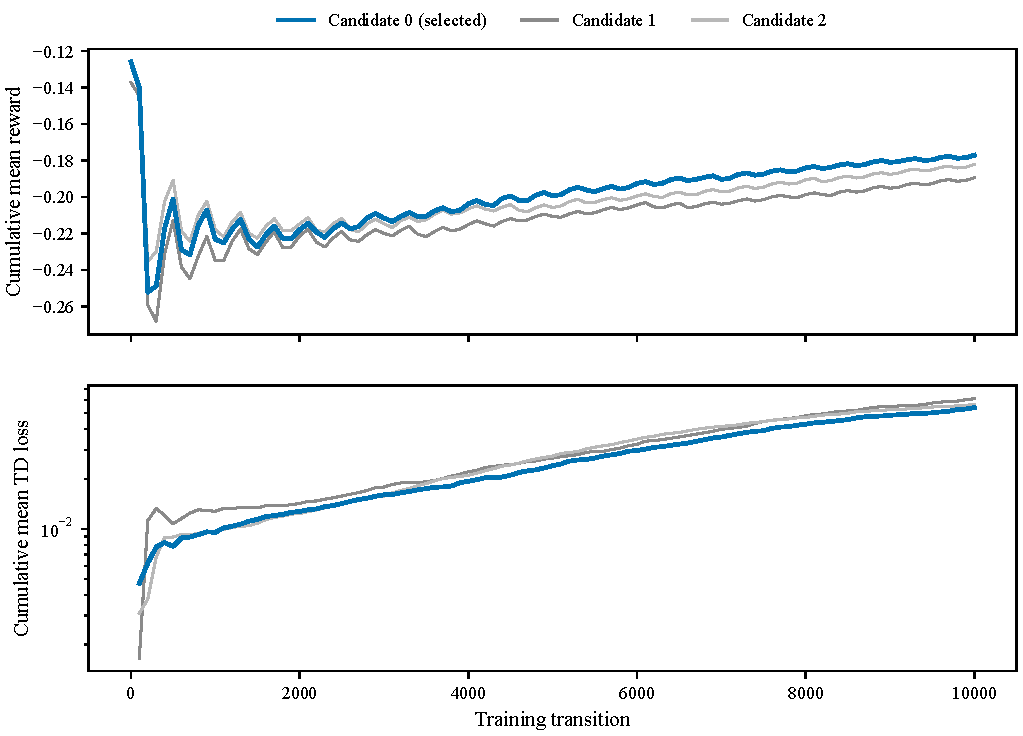
\includegraphics[width=\textwidth]{figures/v3-training-diagnostics.pdf}
  \caption{Development traces for the three v3 candidates.  Candidate 0 was
  selected by the predeclared validation rule and then frozen.  The lower panel
  uses a logarithmic axis for the cumulative mean squared temporal-difference
  (TD) loss.}
  \Description{Two vertically aligned line charts over ten thousand training
  transitions.  The top chart compares cumulative mean reward for three DQL
  candidates and highlights candidate zero.  The bottom chart compares their
  cumulative mean Bellman temporal-difference loss on a logarithmic scale.}
  \label{fig:v3-training-diagnostics}
\end{figure}

The cumulative mean TD loss rises for all three candidates after the early
updates, with all archived values finite and bounded. This is a training
diagnostic, not a convergence result. The target changes with the online
network and the states visited during training, so TD loss measures target
fit rather than model accuracy. Candidate selection used frozen-policy
validation and action coverage. The independent holdout supplies the
comparative performance results below.

\subsection{Independent Holdout Results}

Figure~\ref{fig:v3-scenario-reward} shows that outcomes differ across scenarios.
Frozen DQL has a higher return than the heuristic for
connection-count skew, tiered backlog, and client slowdown.  DQL and the
heuristic are indistinguishable in the pod-pressure scenario because both
select the same effective guarded response.  DQL also matches the static policy
under client slowdown: with client acknowledgement capacity as the bottleneck,
additional connection movement leaves the service-rate bottleneck unchanged.
These control cases identify when the policies provide equivalent outcomes.

\begin{figure}[!htbp]
  \centering
  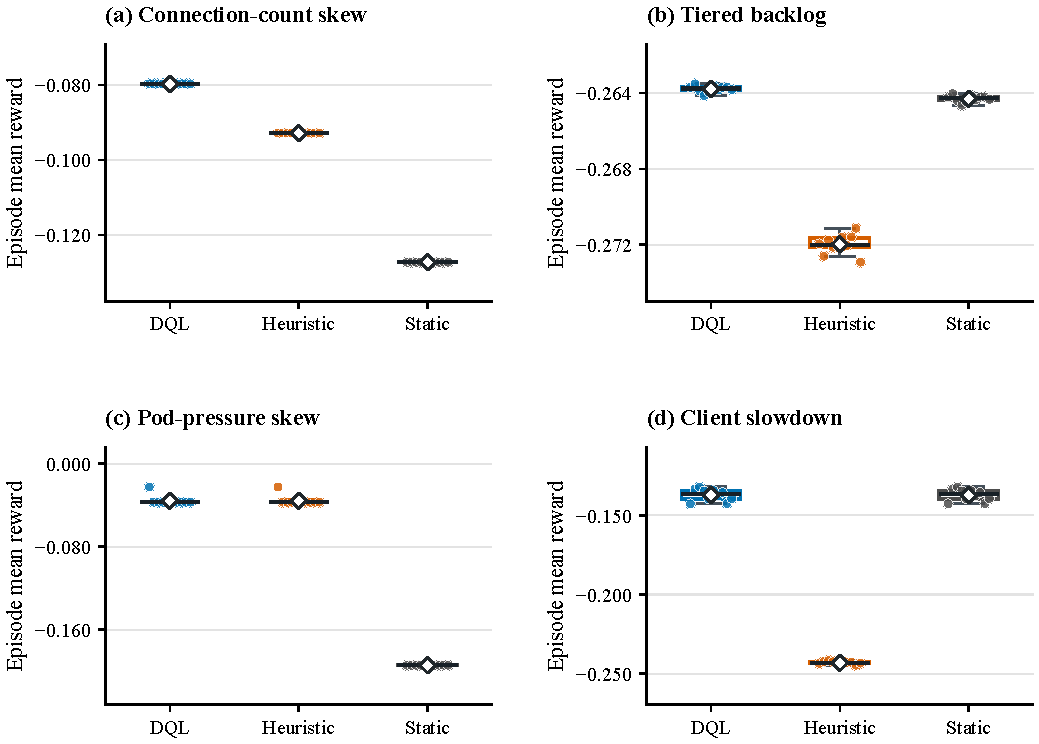
\includegraphics[width=\textwidth]{figures/v3-reward-boxplots.pdf}
  \caption{Holdout reward distributions for frozen DQL, heuristic, and static
  policies. Each panel contains ten paired seeds per policy. Boxes span the
  first and third quartiles, the central line is the median, whiskers extend
  to observations within 1.5 interquartile ranges, and diamonds mark means.
  Every episode is shown as a point, including observations beyond whiskers.
  Panels use separate vertical scales; higher reward is better.}
  \Description{Four box-and-point panels compare episode mean reward across
  connection-count skew, tiered backlog, pod-pressure skew, and client slowdown.
  Constant outcomes in the count-skew scenario collapse to horizontal lines.
  Frozen DQL has higher mean reward than the heuristic in three scenarios and
  equal reward in the pod-pressure scenario.}
  \label{fig:v3-scenario-reward}
\end{figure}

The boxes in Figure~\ref{fig:v3-scenario-reward} describe the distribution of
episode means, not the distribution of individual decision intervals. Horizontal
point offsets separate the ten observations without changing their rewards.
Collapsed boxes in the connection-count scenario reflect identical outcomes,
not missing data. Separate panel scales make the smaller spread in the tiered-backlog case
visible. The paired estimates below provide the statistical comparison, not
the visual height of a box.

Across all 40 paired episodes, frozen DQL improves mean reward over the
heuristic from $-0.1609$ to $-0.1291$.  The mean paired difference is $0.0318$
(bootstrap 95\% CI $[0.0191,0.0455]$), equivalent to a $19.8\%$ relative
benefit under Eq.~\eqref{eq:relative-benefit}; the paired standardized effect is
$d_z=0.729$, and the Holm-adjusted sign-flip $p$-value is below $0.001$.
Table~\ref{tab:v3-paired-effects} and Figure~\ref{fig:v3-paired-benefit} show
that this overall gain comes with tradeoffs.

\begin{table}[!htbp]
  \caption{Frozen DQL versus the heuristic on the independent v3 holdout.
  Positive benefit favors DQL.  CIs are paired-bootstrap intervals transformed
  by Eq.~\eqref{eq:relative-benefit}; $p_H$ is Holm-adjusted over 18 pooled
  metric-by-baseline tests.}
  \Description{Table listing DQL and heuristic means, direction-adjusted
  relative benefits with 95 percent confidence intervals, and Holm-adjusted
  paired sign-flip p-values for nine operational metrics.}
  \label{tab:v3-paired-effects}
  \centering
  \small
  \begin{tabular}{lrrrr}
    \toprule
    Metric & DQL & Heuristic & Benefit [95\% CI] (\%) & $p_H$ \\
    \midrule
    Mean reward & $-0.1291$ & $-0.1609$ & $19.8\ [11.9,28.3]$ & $<.001$ \\
    Backlog ratio & $0.1749$ & $0.2002$ & $12.7\ [-1.2,27.1]$ & $.095$ \\
    Conn.-subscription variance & $574.7$ & $5768.7$ & $90.0\ [61.0,120.8]$ & $<.001$ \\
    Conn.-backlog variance & $2.280\!\times\!10^{13}$ & $1.568\!\times\!10^{13}$ & $-45.4\ [-72.5,-22.6]$ & $.022$ \\
    Subscription imbalance & $0.0898$ & $0.4343$ & $79.3\ [59.1,99.5]$ & $<.001$ \\
    Backlog imbalance & $0.2194$ & $0.1638$ & $-34.0\ [-56.4,-13.6]$ & $.022$ \\
    Combined conn. imbalance & $0.1546$ & $0.2991$ & $48.3\ [33.8,63.8]$ & $<.001$ \\
    Pod pressure & $0.1878$ & $0.2051$ & $8.4\ [3.6,13.6]$ & $.022$ \\
    Throughput ratio & $0.2840$ & $0.2973$ & $-4.5\ [-7.1,-2.2]$ & $.022$ \\
    \bottomrule
  \end{tabular}
\end{table}

\begin{figure}[!htbp]
  \centering
  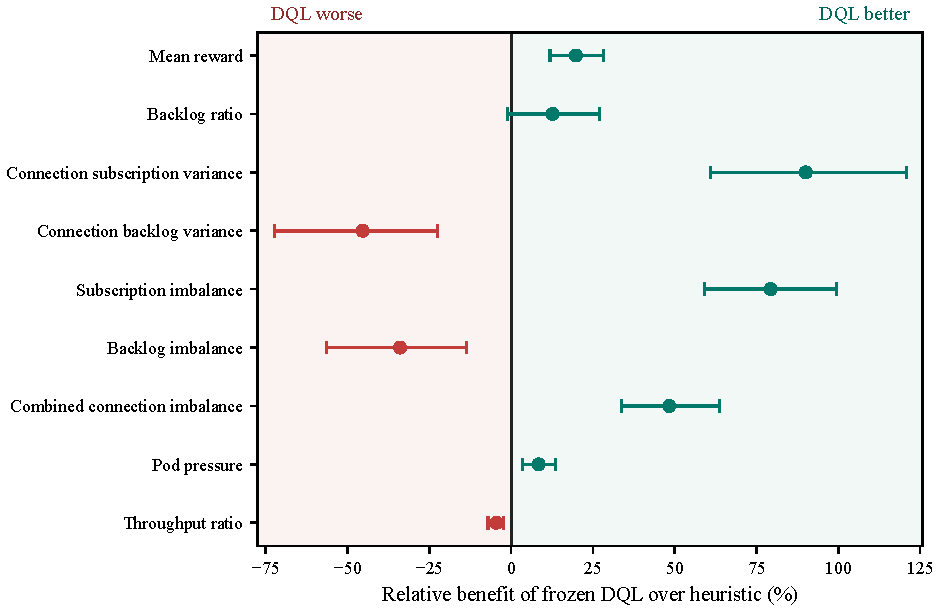
\includegraphics[width=\textwidth]{figures/v3-paired-benefit-forest.pdf}
  \caption{Direction-adjusted relative benefit of frozen DQL over the
  heuristic across 40 paired holdout episodes.  Points are mean effects and
  whiskers are paired-bootstrap 95\% confidence intervals.  Values right of
  zero favor DQL; values left of zero favor the heuristic.}
  \Description{Horizontal forest plot for nine metrics.  DQL improves reward,
  connection subscription variance, subscription imbalance, combined
  connection imbalance, and pod pressure.  Its backlog ratio interval crosses
  zero, while connection backlog variance, backlog imbalance, and throughput
  favor the heuristic.}
  \label{fig:v3-paired-benefit}
\end{figure}

The largest benefit is a $90.0\%$ reduction in connection-level subscription
variance, consistent with the design objective of moving subscriptions away
from overloaded persistent connections.  Subscription imbalance falls by
$79.3\%$, combined connection imbalance by $48.3\%$, and mean pod pressure by
$8.4\%$.  Mean backlog ratio is $12.7\%$ lower, but its interval crosses zero
and the adjusted test is not significant ($p_H=.095$).  Conversely, DQL has
$45.4\%$ higher connection-backlog variance, $34.0\%$ higher normalized backlog
imbalance, and $4.5\%$ lower throughput than the heuristic.  The scalar reward
still favors DQL because its configured penalties place substantial weight on
subscription pressure and combined imbalance. The holdout therefore identifies
a multi-objective advantage for DQL and a queue-drainage advantage for the
heuristic.

\begin{figure}[!htbp]
  \centering
  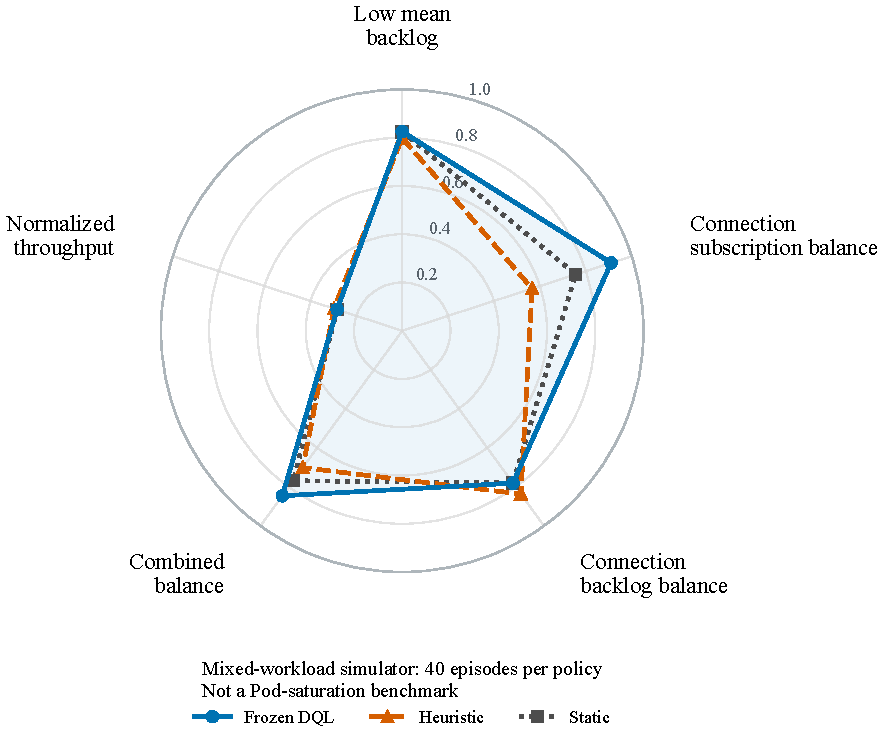
\includegraphics[width=\textwidth]{figures/v3-operational-radar.pdf}
  \caption{Mixed-workload simulator profiles, not a Pod-saturation benchmark,
  across 40 paired holdout episodes per policy. Subscription balance is
  measured across client connections, not across all Pods. All axes use a
  fixed zero-to-one scale with larger values preferred. Backlog and imbalance
  costs are displayed as one minus their mean normalized value; throughput
  retains its recorded normalized value. The profiles are descriptive, not
  an additional weighted score or significance test.}
  \Description{A five-axis radar chart compares frozen DQL, heuristic, and
  static policies. DQL extends farther on subscription and combined balance;
  the heuristic extends farther on backlog balance and throughput. All profiles
  use the same normalization and the full zero-to-one radial range.}
  \label{fig:v3-operational-radar}
\end{figure}

Figure~\ref{fig:v3-operational-radar} summarizes these tradeoffs without mixing
raw variances with event rates. For policy $\pi$ and a normalized cost metric $x_v$,
the plotted coordinate is $1-\bar{x}_{\pi,v}$; the throughput coordinate is
$\bar{x}_{\pi,\mathrm{throughput}}$. Here each mean covers the same 40 episodes,
with ten episodes from each scenario. No observed minimum or maximum is used
to stretch an axis. DQL's stronger subscription and combined balance coexist
with the heuristic's stronger backlog balance and throughput. Polygon area
has no statistical interpretation, and the combined-balance axis is derived
from the two imbalance components rather than being an independent outcome.
Uncertainty and paired comparisons remain those in
Table~\ref{tab:v3-paired-effects} and Figure~\ref{fig:v3-paired-benefit}.

This pooled profile characterizes the mixed workloads; Pod saturation is
evaluated separately. The
connection-count-skew workload has no arrivals or initial backlog and therefore
contributes zero throughput for all policies. In the pod-pressure workload,
all policies serve the offered traffic with essentially zero residual backlog;
their throughput is therefore equal despite different Pod pressure. The
client-slowdown workload is limited by client acknowledgement capacity.
Count balance and recovery of overloaded-Pod bandwidth are therefore separate
endpoints. The saturated scale-out comparison is
reported separately in Figures~\ref{fig:scaleout-backlog-recovery}
and~\ref{fig:scaleout-violin-distributions}.

The distinction is operational, not merely graphical. Equal subscription
counts can leave every persistent socket on the same saturated Pod, and moving
idle subscriptions does not redistribute queued work. Conversely, moving
backlogged subscriptions to a Pod with spare service capacity can raise
aggregate throughput, provided client ACK capacity and shared Queue or network
limits do not become the bottleneck. In the scale-out experiment, the initial
connection counts and backlogs are already balanced
($V_u^N(0)=V_u^G(0)=0$), yet all ten sockets terminate on one Pod. Migration
across Pods raises measured simulator throughput from 58,000 to 219,762 events/s
(3.79 times). Thus, the throughput-recovery evidence is the stressed placement
comparison in Section~\ref{sec:scaleout-recovery}. Connection-balance scores
describe a different property. The Oracle Cloud preload pair in
Section~\ref{sec:ttl-preload-results} measures expiry and ACK completion with
the migration guard held at stay.

The comparison with static control isolates the benefit of rebalancing under
concentrated load. In the 1,600-subscription pod-pressure scenario, three of
four active connections initially terminate on the same pod. Static placement
therefore retains mean pod pressure $1.0125$, whereas DQL promotes a guarded
probe target and reduces it to $0.2176$, a $78.5\%$ reduction. The corresponding
paired reward improvement is $0.1588$ (95\% bootstrap CI
$[0.1573,0.1617]$). In the connection-count-skew scenario, DQL reduces mean
connection subscription-count variance from $6{,}250.0$ to $2{,}298.7$
($63.2\%$) and improves mean reward by $0.0475$. Across all four scenarios,
pooled mean reward improves by $0.0517$ relative to static placement. The
scenario plot also identifies cases where DQL and static placement are equal.
The paired analysis assigns each measured gain to its workload, keeping the
concentrated-load and tiered-backlog results separate.
\FloatBarrier

\subsection{Action-Contract Validation}

The v3 policy passed the declared subscription-count, backlog-rebalancing,
and migration coverage gates. The expanded v4--v6 studies tested all five
interventions and fault guards. None passed every learned-action coverage
gate, although the v6 candidates all passed the safety scenarios. These
completed development studies do not supply additional holdout performance
estimates. Appendix~\ref{app:action-diagnostics} retains their full results,
including the scripted test of the corrected scale-up contract.

\subsection{Adverse-Probe Promotion Ablation}
\label{sec:adverse-probe-ablation}

The retained probe is a candidate endpoint, not an instruction to migrate.
To isolate this distinction, we registered a paired mechanism experiment before
the confirmatory run. In every episode, the probe was set to reach the pod with the highest
initial pressure. The deployment mask evaluated the concrete
source--target pair and rejected $a^{\mathrm{mig}}$ whenever its projected
pressure improvement was below 0.01. The primary ablation then bypassed that
mask for exactly one interval, moved the highest-backlog non-target connection
to the adverse pod, and returned control to the same frozen DQL checkpoint.
Thus, \emph{Frozen DQL} and \emph{DQL + forced promotion} differ only by that
initial override and its subsequent state consequences. \emph{Blind
promotion} makes the same move and then stays; \emph{Static} never changes the
initial placement; and the guarded heuristic uses the same feasibility mask as
DQL.

For total backlog $B(t)$ in the evaluated subscription population over $T$
decision intervals, the primary endpoint is
the normalized trapezoidal backlog area
\begin{equation}
  \mathrm{AUC}_{B}=\frac{1}{T}
  \sum_{t=1}^{T}\frac{B(t-1)+B(t)}{2B(0)}.
  \label{eq:normalized-backlog-auc}
\end{equation}
It measures how much work remains queued over time. Lower values indicate
earlier drainage. The statistical unit is the environment seed, not an interval. The
primary cohort uses 30 previously unused paired seeds and 1,200 subscriptions.

\begin{figure}[!htbp]
  \centering
  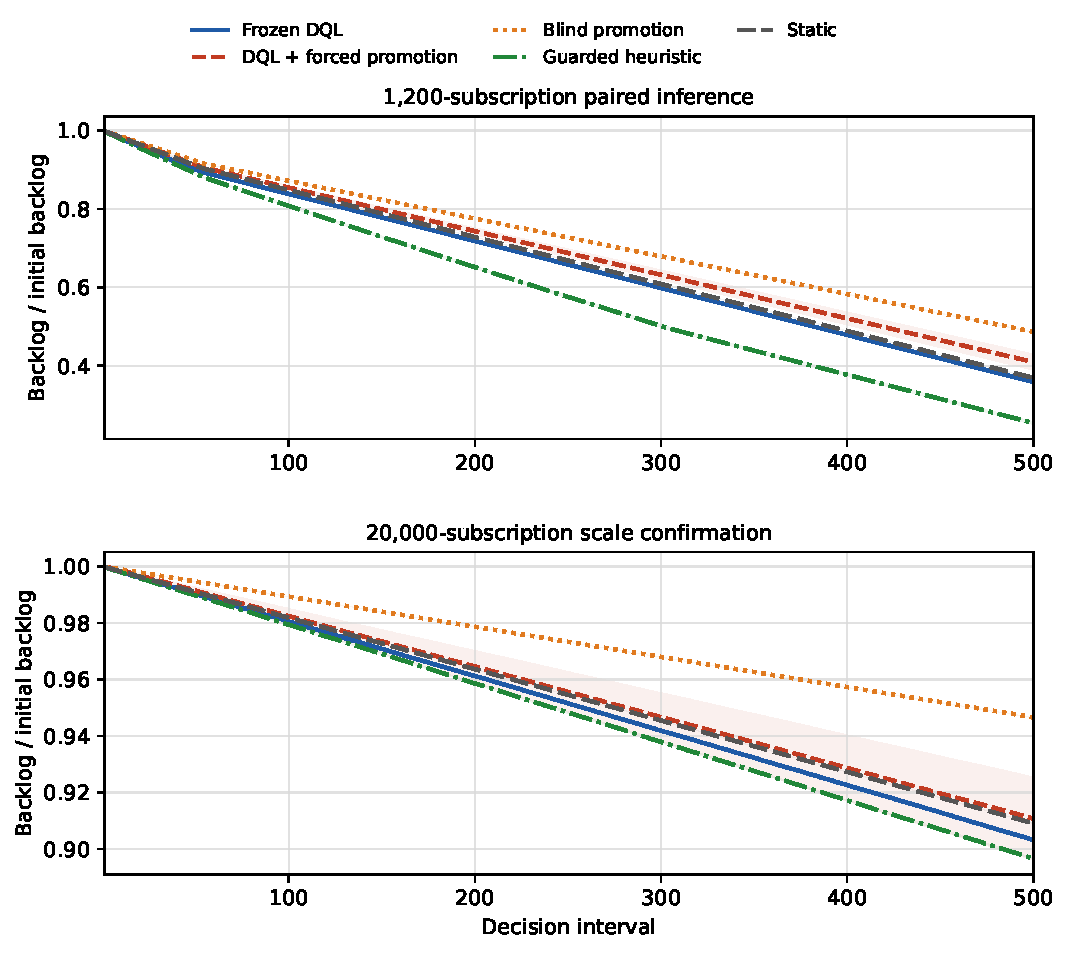
\includegraphics[width=\textwidth]{figures/backlog_trajectories.pdf}
  \caption{Mean normalized backlog trajectories for the adverse-probe
  ablation. Shaded bands are descriptive 95\% normal-approximation intervals
  across paired seeds. The upper panel contains the 30-seed inference cohort;
  the lower panel contains the five-seed 20,000-subscription scale
  confirmation. The forced-promotion policy resumes the same frozen DQL
  controller after the interval-zero override.}
  \Description{Two vertically aligned backlog-ratio line charts compare frozen
  DQL, the same DQL after one forced adverse promotion, blind promotion, a
  guarded heuristic, and static placement. Guarded DQL remains below forced,
  blind, and static placement, while the guarded heuristic drains fastest.}
  \label{fig:adverse-probe-trajectories}
\end{figure}

Each episode runs for 500 intervals. Paired mean differences use 10,000
bootstrap resamples and one-sided sign randomization with 100,000 sign vectors;
Holm adjustment covers the four named baselines. The action mask rejected the
adverse migration in all 30 primary and all five scale-confirmation
environments.

In the primary cohort, guarded DQL attains mean $\mathrm{AUC}_{B}=0.66046$,
compared with 0.68938 after the forced promotion. The paired difference is
$-0.028918$ (95\% CI $[-0.039444,-0.019073]$), a 4.19\% reduction relative to
the forced-promotion ablation. The raw one-sided randomization $p$-value is
$1.0\times10^{-5}$ and the Holm-adjusted value is
$4.0\times10^{-5}$. Guarded DQL also reduces backlog AUC by 9.34\% relative to
blind promotion and by 1.41\% relative to static placement. Its final backlog
ratio is 0.35875, compared with 0.40936, 0.48584, and 0.36864, respectively.
The throughput differences have the same direction: DQL delivers 43.02
million messages, 2.35 million more than the forced-promotion ablation and
5.91 million more than blind promotion.

\begin{table}[!htbp]
  \caption{Adverse-probe ablation outcomes. Backlog AUC and final backlog are
  normalized by initial backlog; lower is better. Throughput is cumulative over
  500 intervals. The 20k cohort is descriptive ($n_{\mathrm{ep}}=5$).}
  \Description{Table comparing mean normalized backlog area, final backlog
  ratio, cumulative throughput, and pod pressure for five policies in the
  1,200-subscription inference and 20,000-subscription scale cohorts.}
  \label{tab:adverse-probe-outcomes}
  \centering
  \resizebox{\textwidth}{!}{%
  \begin{tabular}{llrrrr}
    \toprule
    Cohort & Policy & Backlog AUC & Final ratio & Throughput (M) & Mean pressure \\
    \midrule
    1.2k inference & Frozen DQL & 0.66046 & 0.35875 & 43.02 & 0.5873 \\
    1.2k inference & DQL + forced promotion & 0.68938 & 0.40936 & 40.66 & 0.6100 \\
    1.2k inference & Blind promotion & 0.72853 & 0.48584 & 37.11 & 0.5874 \\
    1.2k inference & Guarded heuristic & 0.59104 & 0.25384 & 47.90 & 0.5941 \\
    1.2k inference & Static & 0.66993 & 0.36864 & 42.56 & 0.5870 \\
    \midrule
    20k confirmation & Frozen DQL & 0.95155 & 0.90316 & 97.05 & 0.7877 \\
    20k confirmation & DQL + forced promotion & 0.95556 & 0.91076 & 91.16 & 0.7884 \\
    20k confirmation & Blind promotion & 0.97323 & 0.94645 & 63.50 & 0.7875 \\
    20k confirmation & Guarded heuristic & 0.94828 & 0.89658 & 102.15 & 0.7883 \\
    20k confirmation & Static & 0.95452 & 0.90903 & 92.50 & 0.7875 \\
    \bottomrule
  \end{tabular}%
  }
\end{table}

\begin{figure}[!htbp]
  \centering
  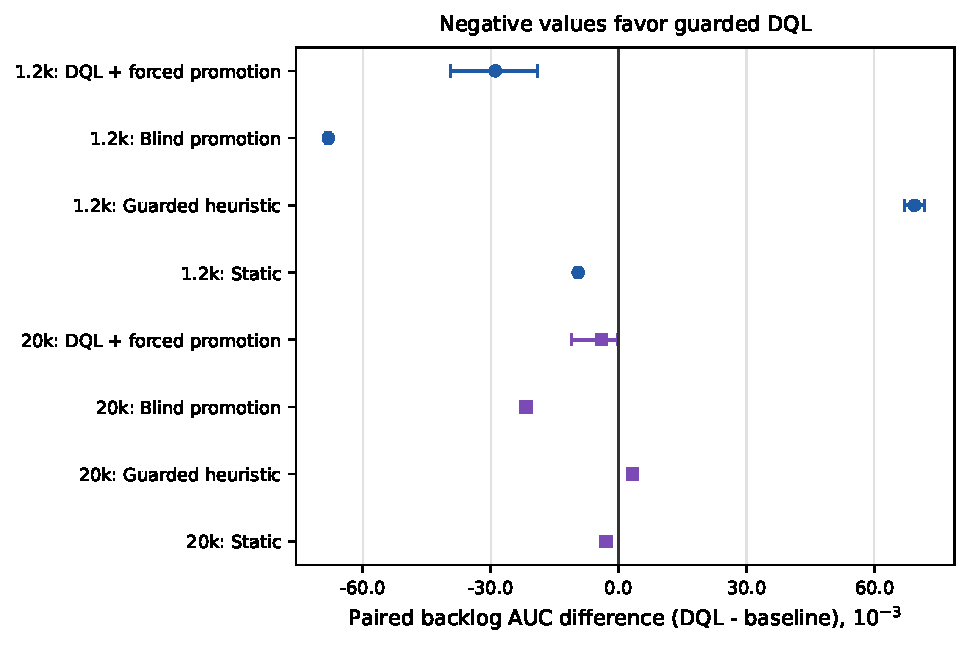
\includegraphics[width=\textwidth]{figures/paired_auc_effects.pdf}
  \caption{Paired normalized backlog-AUC differences between guarded DQL and
  each baseline. Negative values favor DQL; whiskers are paired-bootstrap 95\%
  confidence intervals. Squares denote the descriptive 20,000-subscription
  cohort.}
  \Description{Horizontal forest plot showing DQL below forced promotion,
  blind promotion, and static placement in both cohorts. The heuristic points
  lie above zero, showing that it has lower backlog area than DQL.}
  \label{fig:adverse-probe-effects}
\end{figure}

The heuristic provides an important comparison. Its primary-cohort backlog AUC
is 0.59104, so DQL is 11.75\% higher (paired difference 0.069419, 95\% CI
$[0.066977,0.071826]$). The action records explain the difference. Across 15,000
primary decision intervals, the heuristic executes 2,286 backlog-rebalancing
actions, whereas DQL executes 175 backlog and 175 subscription-count moves and
otherwise stays. In the 20k cohort, the heuristic uses all 625 interventions for backlog rebalancing. DQL splits
625 interventions almost evenly between 315 backlog and 310 subscription-count moves. The backlog-specific measure therefore favors the heuristic, which makes
more backlog-focused moves.
The ablation establishes the benefit of guarding probe promotion; the
backlog-focused heuristic retains the stronger queue-drainage result.

The 20,000-subscription cohort retains the requested four equal groups:
5,000 subscriptions at 100,000 queued messages, 5,000 at 50,000, 5,000 at
5,000, and 5,000 at zero, totaling 775 million initial messages. Guarded DQL
reduces backlog AUC by 0.42\% relative to forced promotion, 2.23\% relative to
blind promotion, and 0.31\% relative to static placement, while remaining
0.34\% above the heuristic. The forced-promotion paired interval lies below
zero, but its exact one-sided $p=0.0625$ and Holm-adjusted $p=0.125$ reflect the
five-seed sample. We consequently treat this cohort as scale confirmation, not
as a second inferential test. The maximum normalized message-conservation
residual over all 175 episodes is $1.031\times10^{-14}$; this verifies simulator
accounting but does not establish loss-free production handoff.
\FloatBarrier

\subsection{Reproducibility and Study Scope}

\paragraph{Reviewer artifact access.}
The accompanying supplementary archive, \texttt{reviewer-evidence.zip},
contains episode-level simulator CSVs, declared protocols, original aggregate
analyses, the frozen 21--32--6 checkpoint, and identifier-free live summaries.
Its README gives the file map and exact offline commands. A Python 3.9+
standard-library script verifies the checksum manifest, checks paired cohort
coverage, recomputes policy means and selected effect sizes, and reconciles
the loaded trial's reported subscription and ACK totals. A separate inference
option evaluates the saved network without transport access or model updates.
The archive supports reanalysis and checkpoint inspection; it does not expose
corporate credentials, raw event payloads, private endpoint identifiers, or
the proprietary service source. It is not a complete independent deployment
rerun. Provenance records distinguish unchanged measurements from redacted
local-path metadata.

The manuscript bundle contains the exact v3 aggregate CSV files, v3--v6 JSON
protocols and summaries, the adverse-probe protocol and episode-level outputs,
and the scripts that regenerate every figure in this section. The
larger private evidence archive additionally records source-file SHA-256 hashes,
frozen-checkpoint hashes, raw episode rows, and a recursive checksum manifest.
The implementation test suite contains unit tests for state construction,
action masks, replay, checkpoint persistence, migration state transitions, and
fault guards, together with a Java STOMP fixture. At the source revision used
for this manuscript, all 267 tests pass, including the four adverse-probe
evaluator tests, cap-restoring scale-up tests, and legacy-policy rejection
tests.

The recovery study includes 20,000 subscriptions and four modeled pods;
the earlier four-scenario holdout contains up to 1,600 subscriptions. These
are simulator measurements with explicit workload and service assumptions.
The v4--v6 all-action studies ended at their development coverage gates and
are reported as diagnostics, separate from holdout performance. The Oracle
Cloud cluster experiment in Section~\ref{sec:mumbai-experiment} measures
20,000-subscription topology and ten live handoffs using existing queued
events rather than the simulator's paired, controlled workloads. The
backlog-recovery effect sizes therefore apply to the stated simulator. The
Oracle Cloud measurements establish execution of the corresponding
connection-replacement mechanism in Kubernetes.
The additional loaded scale-out run in Section~\ref{sec:live-dql-scaleout}
records three selective DQL handoffs and 8,000 acknowledged STOMP deliveries
for 1,000 subscriptions. It uses a fixed client-processing delay and bounded
publication, and supplies functional handoff evidence rather than a matched
throughput effect size.

\FloatBarrier



\section{Stability Controls and Policy Validation}

Because the controller operates with partial and periodically refreshed
statistics, stability is enforced at two levels.  During learning, replay,
target-network synchronization, bounded rewards, and epsilon decay limit the
rate at which value estimates change.  During execution, feasibility masks,
minimum-improvement thresholds, cooldowns, and the receipt-gated handoff protocol
prevent a high Q-value from bypassing required operating rules. These controls
bound the available transitions. Their role is operational stability, distinct
from a proof of learned-policy convergence.

Classical tabular Q-learning guarantees assume a stationary, fully observable
Markov decision process and sufficient visitation of every state-action pair.
The client instead receives delayed partial observations in an environment
whose queue arrivals, acknowledgement capacity, and competing clients can
change. Policy quality is therefore evaluated under the stated workloads,
without a global-optimality guarantee. The finite v3 traces describe training
behavior rather than Bellman-loss convergence. The v4--v6 results distinguish
training completion from action coverage. The validation protocol uses
action-coverage, fault-safety, churn, and performance gates to assess each
frozen policy.

\section{Discussion}

The main systems finding is that subscriber capacity and client access to that
capacity are separate. Adding Pods supplies service capacity; moving existing
subscription-bearing connections makes it reachable by persistent clients.
The guarded-greedy and DQL policies both achieve this in the scale-out model.
Their nearby throughput results support the shared mechanism rather than
requiring a claim that learning beats a strong greedy rule in every workload.

Policy choice depends on the operational objective. Greedy control gives a
direct, inspectable response to measured pressure. DQL can account for delayed
costs and several competing objectives. A subscription move changes future
backlog distribution; migration trades immediate handoff cost for later
capacity. Both selectors operate above the same bounded, checked actions.

QEdgeProxy selects service instances using client QoS feedback
\cite{Cilic2025}, while Yahya et al. adapt offloading through decentralized
bandits and server-reward adjustment \cite{Yahya2024}. The present work
focuses on subscription-aware persistent messaging clients under partial
observability and treats connection-level rebalancing as a first-class
control action alongside endpoint selection. This distinction
matters operationally: endpoint selection chooses the serving Pod, while
connection-level rebalancing corrects subscription skew within the client.

The holdout results show how learning compares with the heuristic.
Both policies can perform the same actions, so they can reach the same
capacity limit in some scenarios.  DQL's measured advantage is concentrated
in subscription distribution, combined connection imbalance, and avoiding a
harmful heuristic intervention during client slowdown.  The heuristic retains
an advantage in throughput and backlog-distribution metrics. These results
identify the operating objectives favored by each policy. The
component-level analysis reports these tradeoffs alongside the scalar reward;
policy selection uses development validation before the holdout is evaluated.

The distinction between a model's quality and the utility of the complete
system also appears in Casimiro et al.'s probabilistic framework for adapting
ML components \cite{Casimiro2024ModelChecking}. In our setting, a favorable
Q-value is therefore interpreted alongside backlog, throughput, and handoff
outcomes. Gheibi and Weyns introduce a lifelong-learning
layer to respond to changing adaptation options
\cite{Gheibi2024AdaptationDrift}. Our experiments evaluate a fixed policy under
the stated workload and deployment conditions. Lifelong adaptation is outside
this study's scope.

The loaded Oracle Cloud scale-out trial adds direct evidence for selective
execution (Section~\ref{sec:live-dql-scaleout}). Every handoff preserved three
unselected active sessions, while the full cohort reached 8,000 ACK receipts.
The measured drain waits also show why opening a replacement socket is only
one part of migration: client processing and acknowledgement completion can
dominate the handoff duration. These measurements validate the learned
decision-to-execution path under the declared load and processing limit.

The action-contract studies provide a further design lesson: a useful
executor and a policy that reliably selects it are separate requirements.
The cap-restoring scale-up preflight improved reward and maximum subscription
count, but the expanded learner study did not pass every coverage gate.
Appendix~\ref{app:action-diagnostics} retains these results. They explain why
the live checkpoint uses a compatible, restricted rebalancing profile.

\section{Conclusion}

We presented a probe-guided, client-side framework for rebalancing
persistent subscription connections without requiring cluster-wide client
visibility.  The mechanism combines per-subscription queues, active-connection
telemetry, and a load-balancer-assigned probe. Greedy rules or DQL select
bounded actions, and a shared executor carries out receipt-gated handoff.
The technical contribution is the link between partial observations,
endpoint-preserving probe promotion, and selective subscription reassociation.

The primary experiment demonstrates recovery after a one-to-four pod capacity
increase with 20,000 subscriptions and 775 million queued events. Guarded-greedy
migration and frozen DQL deliver 221,260 and 219,762 events/s, respectively,
compared with 58,000 events/s for unchanged placement. Frozen DQL
uses all four pods, delivers 3.79 times the mean throughput, and leaves 27.52\%
less backlog after 20 minutes than retaining the ten original connection
assignments. Its 12.30\% reduction in backlog area satisfies the registered
paired statistical criterion. The adverse-probe ablation complements this
result: evaluating the candidate before promotion reduces backlog area by
4.19\% relative to forcing one harmful migration.

These findings identify the operational benefit of the mechanism: scaled-out
subscriber capacity becomes useful to existing subscriptions through
client-directed connection reassociation, while combined subscription and
backlog pressure determines whether a sampled target is suitable. The
supporting studies characterize policy tradeoffs and action coverage.
The mixed-workload holdout favors DQL in composite reward and subscription
balance, while the heuristic favors throughput and backlog balance. These
results support two evaluated policy options rather than universal DQL
superiority or an untested DQL-tuned scripted policy.
The isolated Oracle Cloud cluster qualification also demonstrates a 60\% reduction in source
subscriptions through three full-connection migrations, with all 2,000
subscriptions retained and 73,639 observed deliveries reconciled at closure.
Its startup measurements explicitly capture activation while deliveries flow.
A further loaded one-to-four-Pod trial retained all 1,000 subscriptions and
four active connections through three DQL-selected handoffs. Each action
preserved the other three sessions. The final client distribution was 500,
250, 250 and zero across the four available Pods, with 8,000 observed
deliveries acknowledged and no unresolved client deliveries at closure.
A separate Oracle Cloud preload pair measured twelve native TTL interruptions
and 89.44\% ACK-receipt completion, versus no interruptions and 100\% completion
in the TTL-disabled DQL arm (Section~\ref{sec:ttl-preload-results}). That arm
remained at guard-held \emph{stay}: a 200-second minimum telemetry sweep exceeded
the 180-second freshness deadline. The result measures expiry-related receipt
completion under the telemetry constraint. The comparative throughput and
backlog-recovery gains are simulator measurements under the stated service
assumptions. The Oracle Cloud experiments establish live handoff execution,
subscription retention, and observed delivery behavior. Together, these studies
describe the mechanism's measured benefits and the operating conditions under
which they were obtained.

\FloatBarrier
\appendix
\Needspace{16\baselineskip}
\section{Notation Reference}
\label{app:notation}
The tables collect the detailed definitions used in the model and experimental endpoints.

\Needspace{12\baselineskip}
\begingroup
\small
\renewcommand{\arraystretch}{1.12}
\setlength{\tabcolsep}{5pt}
\begin{longtable}{|>{\raggedright\arraybackslash}p{0.29\linewidth}|>{\raggedright\arraybackslash}p{\dimexpr0.71\linewidth-4\tabcolsep-3\arrayrulewidth\relax}|}
\caption{Summary of Notations: System Sets and Pod Pressure}\label{tab:notation}\\
\hline
\textbf{Symbol} & \textbf{Description} \\ \hline
\endfirsthead
\caption[]{Summary of Notations: System Sets and Pod Pressure (continued)}\\
\hline
\textbf{Symbol} & \textbf{Description} \\ \hline
\endhead
\multicolumn{2}{r}{\footnotesize Continued on next page}\\
\endfoot
\endlastfoot
\multicolumn{2}{|c|}{\textbf{Server-Level Placement Variables}} \\ \hline
		
		$\mathcal{S}=\{1,\ldots,n\}$, $\mathcal{U}=\{1,\ldots,m\}$
		& Sets of Pod indices and client indices; $n$ and $m$ are their counts \\ \hline

		$t$, $T$, $\Delta$
		& Decision-epoch index, last epoch, and seconds per epoch; adjacent epochs are $t$ and $t+1$ \\ \hline

		$\mathcal{K}_u(t)$, $\mathcal{C}_u(t)$
		& Client $u$'s subscription set and active delivery-connection set \\ \hline

		$\mathcal{K}_{u,c}(t)$, $z_{u,k,c}(t)$
		& Subscriptions assigned to connection $c$ and the binary indicator of that assignment \\ \hline

		$Q_{u,k}(t)$, $b_{u,k}(t)$
		& Subscription queue and its backlog count, $b_{u,k}(t)=|Q_{u,k}(t)|$ \\ \hline

		$i_{u,c}(t)$, $\mathcal{O}_u(t)$
		& Pod index reached by connection $c$ and set of Pod indices observed by client $u$ \\ \hline

		$p_i$, $y_i(t)$
		& Pod name and reported tuple $(p_i,X_i(t),B_i(t),H_i)$; $y_i(t)$ is not the scalar Bellman target $y_t$ \\ \hline

		$\mathcal{R}_i(t)$
		& Set of server-side subscription queues currently served by pod $i$ \\ \hline

		$\tilde{b}_{i,r}(t)$
		& Backlog of server-side subscription queue $r\in\mathcal{R}_i(t)$ \\ \hline

		$X_i(t)$
		& Pod-level subscription count for pod $i$ \\ \hline

		$B_i(t)$
		& Cumulative backlog over all subscription queues served by pod $i$ \\ \hline

		$H_i$
		& Configured maximum processing threshold for Pod $i$ in events/s, used as a normalization signal \\ \hline

		$X_{\mathrm{safe}}$
		& Subscription-count level after which pod reliability risk begins to increase \\ \hline

		$X_{\mathrm{hard}}$
		& Hard subscription-count reference used to normalize severe subscription pressure, with $X_{\mathrm{hard}}>X_{\mathrm{safe}}$ \\ \hline

		$B_{\mathrm{ref}}$
		& Reference backlog used to normalize pod backlog pressure \\ \hline

		$P^X_i(t)$
		& Normalized pod subscription-count pressure \\ \hline

		$P^B_i(t)$
		& Normalized pod cumulative-backlog pressure \\ \hline

		$P^H_i(t)$
		& Backlog pressure normalized by $H_i\Delta+\varepsilon_0$, then clipped at one \\ \hline

		$\varepsilon_0$, $[x]_+$
		& Positive denominator offset in messages and positive part $\max\{x,0\}$; distinct from exploration probability $\epsilon$ \\ \hline

		$P^R_i(t)$
		& Nonlinear pod reliability-risk pressure caused by excessive subscription count \\ \hline

		$P_i(t)$
		& Weighted pod pressure score used in the deployable reward \\ \hline

		$\omega_X,\omega_B,\omega_H,\omega_R$
		& Nonnegative weights for subscription-count, backlog, threshold-relative backlog, and reliability-risk pressure terms \\ \hline
\end{longtable}
\endgroup

\Needspace{12\baselineskip}
\begingroup
\small
\renewcommand{\arraystretch}{1.12}
\setlength{\tabcolsep}{5pt}
\begin{longtable}{|>{\raggedright\arraybackslash}p{0.29\linewidth}|>{\raggedright\arraybackslash}p{\dimexpr0.71\linewidth-4\tabcolsep-3\arrayrulewidth\relax}|}
\caption{Summary of Notations: DQL Observation and Reward Symbols}\label{tab:notation_dql}\\
\hline
\textbf{Symbol} & \textbf{Description} \\ \hline
\endfirsthead
\caption[]{Summary of Notations: DQL Observation and Reward Symbols (continued)}\\
\hline
\textbf{Symbol} & \textbf{Description} \\ \hline
\endhead
\multicolumn{2}{r}{\footnotesize Continued on next page}\\
\endfoot
\endlastfoot
$J_T$
		& Offline finite-horizon system evaluation cost over epochs $0,\ldots,T$ \\ \hline

		$\Phi_X(t)$
		& Pod subscription-count variance across the cluster at time $t$ \\ \hline

		$M(t)$
		& Total number of migration or reconnect operations during epoch $t$ \\ \hline

		$\Lambda_B,\Lambda_X,\Lambda_C,\Lambda_M$
		& Nonnegative weights in the offline evaluation objective for backlog, pod balance, connection balance, and migration churn \\ \hline
		
		$T_u(t)$ 
		& Effective client-side throughput from delivered, processed, and acknowledged messages \\ \hline
		
		$R_u(t)$ 
		& Deployable reward observed by client $u$ at time $t$ \\ \hline
		
		$Q_\theta(o,a)$ 
		& Online DQL action-value network used for action selection and gradient updates \\ \hline

		$Q_{\theta^-}(o,a)$
		& Target DQL action-value network used only to compute Bellman targets \\ \hline

		$\theta,\theta^-$
		& Online-network parameters and delayed target-network parameters \\ \hline

		$\mathcal{D}$, $\xi_t$
		& Replay buffer and transition $(o_u(t),a_u(t),R_u(t),o_u(t+1))$ \\ \hline

		$y_t$, $\mathcal{L}(\theta)$
		& Scalar Bellman target and mean squared temporal-difference loss \\ \hline

		$\alpha$, $K_{\mathrm{sync}}$
		& Online-network learning rate and target-copy interval in training updates \\ \hline
		
		$\gamma$ 
		& DQL discount factor \\ \hline
		
		$\epsilon$ 
		& Exploration probability in the DQL epsilon-greedy action policy \\ \hline
		
		$\delta$ 
		& Required Q-value improvement of migration over stay; distinct from variance thresholds $\gamma_N,\gamma_G$ \\ \hline
		
		$\lambda_1,\ldots,\lambda_7$ 
		& Weight coefficients used in the deployable reward function \\ \hline
		
		$o_u(t)$ 
		& Client observation vector used by the DQL policy \\ \hline

		$o^B_u(t)$
		& Backlog observation branch containing normalized local backlog and backlog growth features \\ \hline

		$o^N_u(t)$
		& Subscription-count observation branch containing normalized $N_{u,c}(t)$ and $V^N_u(t)$ features \\ \hline

		$o^G_u(t)$
		& Backlog-load imbalance observation branch containing normalized $G_{u,c}(t)$ and $V^G_u(t)$ features \\ \hline

		$o^C_u(t),o^P_u(t),o^D_u(t)$
		& Connection-count/throughput, pod-pressure, and decision-state observation branches \\ \hline
		
		$\mathcal{A}$ 
		& Set of bounded DQL action templates \\ \hline

		$\mathcal{A}^{\mathrm{adm}}_u(t)$
		& Subset of action templates admitted by client $u$'s guards at time $t$, used for action selection and next-state Bellman maximization \\ \hline

		$i^{\mathrm{probe}}_u(t)$
		& Pod endpoint bound to client $u$'s currently retained, load-balancer-assigned probe socket \\ \hline

		$a_u(t)$, $a'$
		& Selected action at epoch $t$ and candidate next-epoch action in Bellman maximization \\ \hline
\end{longtable}
\endgroup

\Needspace{12\baselineskip}
\begingroup
\small
\renewcommand{\arraystretch}{1.12}
\setlength{\tabcolsep}{5pt}
\begin{longtable}{|>{\raggedright\arraybackslash}p{0.29\linewidth}|>{\raggedright\arraybackslash}p{\dimexpr0.71\linewidth-4\tabcolsep-3\arrayrulewidth\relax}|}
\caption{Summary of Notations: Connection Scaling and Local Counters}\label{tab:notation_connection}\\
\hline
\textbf{Symbol} & \textbf{Description} \\ \hline
\endfirsthead
\caption[]{Summary of Notations: Connection Scaling and Local Counters (continued)}\\
\hline
\textbf{Symbol} & \textbf{Description} \\ \hline
\endhead
\multicolumn{2}{r}{\footnotesize Continued on next page}\\
\endfoot
\endlastfoot
\multicolumn{2}{|c|}{\textbf{Connection Scaling Variables}} \\ \hline
		
		$C(t)$ 
		& Number of active persistent delivery connections for client $u$ at time $t$, $C(t)=|\mathcal{C}_u(t)|$ \\ \hline
		
		$C_{\max}$ 
		& Maximum allowable client connections \\ \hline
		
		$N_{\mathrm{sub}}(t)$ 
		& Total number of active subscriptions maintained by client $u$ at time $t$, $N_{\mathrm{sub}}(t)=|\mathcal{K}_u(t)|$ \\ \hline
		
		$\Theta_N$ 
		& Maximum desired subscription count per connection used by the scaling rule \\ \hline
		
		$\beta$ 
		& Backlog threshold per subscription \\ \hline
		
		$b_{u,k}(t)$
		& Client-observed backlog of subscription queue $k$ for client $u$ \\ \hline
		
		$C_{\mathrm{sub}}(t)$ 
		& Required connections based on total subscription count \\ \hline
		
		$C_k(t)$ 
		& Client connection-count requirement triggered by subscription $k$'s backlog; not multiple owners for that queue \\ \hline

		$C_{\mathrm{back}}(t)$, $C^\star(t)$
		& Maximum backlog-based requirement and desired connection count after combining scaling requirements \\ \hline

		$c^{\mathrm{place}}$, $c^\star$
		& Connection chosen for new-subscription placement and connection evaluated for migration \\ \hline

		$\widehat{N}_{u,c}(t)$, $\widehat{G}_{u,c}(t)$
		& Normalized subscription-count and backlog loads used by the placement score \\ \hline

		$B_u(t)$, $\mathrm{Grow}_u(t)$
		& Sum of client $u$'s subscription backlogs and its positive increase since the previous epoch \\ \hline

		$T^{\mathrm{del}}_u(t)$, $T^{\mathrm{proc}}_u(t)$, $T^{\mathrm{ack}}_u(t)$
		& Delivered, processed, and acknowledged message rates in events/s; their minimum is $T_u(t)$ \\ \hline

		$\widehat{B}_u(t)$, $\widehat{\mathrm{Grow}}_u(t)$, $\widehat{T}_u(t)$
		& Normalized backlog, backlog growth, and throughput under the experiment's stated scaling convention \\ \hline

		$M_u(t)$, $\widehat{C}_u(t)$
		& Migration indicator or normalized count, and active connection fraction $C(t)/C_{\max}$ \\ \hline
\end{longtable}
\endgroup

\Needspace{12\baselineskip}
\begingroup
\small
\renewcommand{\arraystretch}{1.12}
\setlength{\tabcolsep}{5pt}
\begin{longtable}{|>{\raggedright\arraybackslash}p{0.29\linewidth}|>{\raggedright\arraybackslash}p{\dimexpr0.71\linewidth-4\tabcolsep-3\arrayrulewidth\relax}|}
\caption{Summary of Notations: Connection Rebalancing Symbols}\label{tab:notation_rebalancing}\\
\hline
\textbf{Symbol} & \textbf{Description} \\ \hline
\endfirsthead
\caption[]{Summary of Notations: Connection Rebalancing Symbols (continued)}\\
\hline
\textbf{Symbol} & \textbf{Description} \\ \hline
\endhead
\multicolumn{2}{r}{\footnotesize Continued on next page}\\
\endfoot
\endlastfoot
\multicolumn{2}{|c|}{\textbf{Connection-Level Rebalancing Variables}} \\ \hline
		
		$N_{u,c}(t)$
		& Number of subscriptions of client $u$ assigned to connection $c$ at time $t$ \\ \hline

			$G_{u,c}(t)$
			& Cumulative backlog load on connection $c$, computed from the subscription queues assigned to that connection \\ \hline

			$c_h,c_l$
			& Source high-load connection and target low-load connection used in a rebalancing move \\ \hline

			$V^N_u(t)$
			& Connection-level subscription-count variance across client $u$'s active persistent connections \\ \hline

			$\bar{N}_u(t)$, $\bar{G}_u(t)$
			& Mean subscription count and mean cumulative backlog across client $u$'s active connections \\ \hline

			$V^G_u(t)$
			& Connection-level backlog-load variance across client $u$'s active persistent connections \\ \hline

			$\widehat{V}^N_u(t),\widehat{V}^G_u(t)$
			& Normalized subscription-count and backlog-load variance terms used in the local imbalance score \\ \hline

			$V^N_{\mathrm{ref}},V^G_{\mathrm{ref}}$
			& Positive variance references used to normalize $V^N_u(t)$ and $V^G_u(t)$ \\ \hline

			$\sigma^{N}_{\mathrm{tol}}$
			& Tolerable standard deviation of subscription counts across a client's active connections \\ \hline

			$\sigma^{G}_{\mathrm{tol}}$
			& Tolerable standard deviation of cumulative backlog load across a client's active connections \\ \hline

			$\Delta_N$
			& Operator-chosen tolerable spread between a heavy and a light connection in subscription count \\ \hline

			$\Delta_G$
			& Operator-chosen tolerable spread between a heavy and a light connection in cumulative backlog messages \\ \hline

			$\widehat{r}^{\mathrm{ack}}_{u}$
			& Conservative client-observed ACK or message-processing rate for client $u$ \\ \hline

			$\tau_G$
			& Acceptable additional drain-time skew used to derive a latency-driven backlog spread \\ \hline

			$\rho_N$
			& Fraction of $\Theta_N$ used to set the default subscription-count imbalance tolerance \\ \hline

			$\rho_G$
			& Fraction of $\beta\Theta_N$ used to set the default backlog-load imbalance tolerance \\ \hline

			$V_u(t)$
			& Weighted local connection-imbalance score for client $u$ \\ \hline

			$\eta_N,\eta_G$
			& Nonnegative weights for subscription-count imbalance and backlog-load imbalance, with $\eta_N+\eta_G=1$ \\ \hline
			
			$\gamma_N,\gamma_G$ 
			& Thresholds triggering subscription-count and backlog-based connection rebalancing \\ \hline
\end{longtable}
\endgroup
\Needspace{12\baselineskip}
\begingroup
\small
\renewcommand{\arraystretch}{1.12}
\setlength{\tabcolsep}{5pt}
\begin{longtable}{|>{\raggedright\arraybackslash}p{0.29\linewidth}|>{\raggedright\arraybackslash}p{\dimexpr0.71\linewidth-4\tabcolsep-3\arrayrulewidth\relax}|}
\caption{Summary of Notations: Handoff and Experimental Endpoints}\label{tab:notation_handoff_metrics}\\
\hline
\textbf{Symbol} & \textbf{Description} \\ \hline
\endfirsthead
\caption[]{Summary of Notations: Handoff and Experimental Endpoints (continued)}\\
\hline
\textbf{Symbol} & \textbf{Description} \\ \hline
\endhead
\multicolumn{2}{r}{\footnotesize Continued on next page}\\
\endfoot
\endlastfoot
$\mathcal{K}_{\mathrm{move}}$, $s_b$, $s_f$
		& Selected subscription set, barrier timestamp after source quiescence, and source telemetry-frame timestamp \\ \hline
		$I_{c_h,k}(s_f)$, $\operatorname{state}_{c_h,k}(s_f)$
		& Source-reported in-flight count and delivery state for subscription $k$ at frame time $s_f$ \\ \hline
		$c_p$, $i_h$, $i_l$
		& Probe socket and Pod indices reached by $c_h$ and $c_l$ in the architecture figure \\ \hline
		$\ell_k^{\mathrm{act}}$, $t_k^{\mathrm{send}}$, $t_k^{\mathrm{ready}}$
		& Activation latency and submission/receipt timestamps in seconds; $\ell_k^{\mathrm{act}}=t_k^{\mathrm{ready}}-t_k^{\mathrm{send}}$ \\ \hline
		$A^{\mathrm{act}}(s)$
		& Number of receipt-confirmed activations by elapsed time $s$ in seconds \\ \hline
		$t_c^{\mathrm{open}}$, $t_c^{\mathrm{exp}}$, $T_{\mathrm{TTL}}$, $J_c$
		& Connection opening and nominal expiry timestamps, TTL in seconds, and integer jitter in minutes \\ \hline
		$d_c$, $h_c$, $r_c$
		& Disconnect, replacement-CONNECTED, and full binding-restoration timestamps in seconds \\ \hline
		$T_c^{\mathrm{conn}}$, $T_c^{\mathrm{restore}}$
		& Transport reconnect and full restoration durations, measured from $d_c$ \\ \hline
		$T_u^{\mathrm{handoff}}$, $T_u^{\mathrm{drain}}$
		& Measured total handoff and source-drain durations for client $u$ in seconds \\ \hline
		$\mathcal{C}_0$, $I_c(s)$, $F(s)$
		& Initial trial connection pool, unrestored-connection indicator, and affected fraction at elapsed time $s$ \\ \hline
		$D_{\mathrm{obs}}$, $A_{\mathrm{conf}}$
		& Recorded delivery attempts and attempts with confirmed ACK receipts \\ \hline
		$B(t)$, $\mathrm{AUC}_B$
		& Total backlog in the evaluated population and its normalized trapezoidal area over $T$ intervals \\ \hline
		$Y_{\pi,j,v}$, $d_v$, $D_{j,v}$
		& Episode mean for policy $\pi$, episode $j$, metric $v$; benefit direction; and signed paired difference \\ \hline
		$\mathrm{RB}_v$, $p_H$, $d_z$
		& Relative benefit in percent, Holm-adjusted $p$-value, and paired standardized mean difference \\ \hline
		$J$, $R^{\mathrm{train}}_\ell$
		& Number of logged training transitions and the reward recorded for transition $\ell$ \\ \hline
		$M^{\mathrm{ep}}$, $n_{\mathrm{ep}}$
		& Migration count in one episode and number of sampled episodes, distinct from client count $m$ and Pod count $n$ \\ \hline
		$W_1,b_1,W_2,b_2$, $h(o)$
		& Weights and biases of the 21--32--6 Q-network, and its single ReLU hidden representation \\ \hline
		$\mathbf{q}_\theta(o)$
		& Vector of online Q-values, one per action in $\mathcal{A}$, with $o=o_u(t)$ \\ \hline
\end{longtable}
\endgroup

\FloatBarrier
\section{Evaluated Features and Policy Settings}
\label{app:feature-order}

The frozen network consumes the ordered 21-element vector in
Table~\ref{tab:feature-order}. For nonnegative $x$ and positive reference $r$,
the implementation uses $\operatorname{clip}(x/r)=\min(1,x/r)$ and
$\operatorname{lognorm}(x;r)=\min(1,\log(1+x)/\log(1+r))$.
These are numerical scaling rules, not drain-time estimates. A pressure
feature can exceed one through the quadratic reliability term even though
its count, backlog, and capacity components are clipped.

\begin{table}[!htbp]
\centering\small
\caption{Exact input order of the evaluated 21--32--6 network. Indices are
one-based; ``mean'' and ``maximum'' refer to active client connections.}
\Description{Feature indices map to backlog, count and backlog imbalance,
connection cost and throughput, observed Pod pressure, and decision context.}
\label{tab:feature-order}
\begin{tabular}{p{0.09\textwidth}p{0.82\textwidth}}
\toprule
Indices & Features, in order\\
\midrule
1--2 & Log-normalized client backlog; log-normalized positive backlog growth\\
3--5 & Mean and maximum of $\operatorname{clip}(N_{u,c}/\Theta_N)$; $\widehat V_u^N$\\
6--9 & Mean and maximum of $\operatorname{lognorm}(G_{u,c};B_{\mathrm{ref}})$; $\widehat V_u^G$; combined imbalance $V_u$\\
10--11 & $|\mathcal C_u|/C_{\max}$ clipped at one; client throughput divided by the declared throughput reference and clipped at one\\
12 & Active-Pod pressure, weighted by this client's subscription counts on each observed Pod; unweighted mean if the count is zero\\
13--15 & Probe pressure; clipped probe subscription count relative to $X_{\mathrm{safe}}$; clipped probe backlog relative to $B_{\mathrm{ref}}$\\
16--18 & Probe-present indicator; probe endpoint absent from active endpoints; cooldown-ready indicator\\
19--21 & Maximum active telemetry/backlog age ratio; probe age ratio; previous-action-was-migration indicator\\
\bottomrule
\end{tabular}
\end{table}

Pod-wide values are deduplicated when several sockets reach one Pod.
Client backlog sums each known subscription once. When per-subscription
values are absent, the builder uses the active-connection backlog aggregates.
Age ratios are clipped at one. Missing probe data sets its pressure and age
features to one and its present indicator to zero; the independent validity
checks prohibit migration. Coverage and freshness checks are execution gates,
not additional neural inputs.

For the simulator adapter, $B_{\mathrm{ref}}$ is the declared initial tiered
backlog when it is positive, otherwise $\max(1,\beta|\mathcal K_u|)$.
The growth reference equals $B_{\mathrm{ref}}$;
$V^N_{\mathrm{ref}}=(0.2\Theta_N)^2$ and
$V^G_{\mathrm{ref}}=(0.2B_{\mathrm{ref}})^2$.
The safe and hard subscription thresholds are $2\Theta_N$ and
$\max(2\Theta_N+1,\operatorname{round}(2.5\Theta_N))$.
The throughput reference is three times the configured base client ACK rate.
These constants are scenario inputs, not fitted from holdout outcomes.
The service-model pressure used to generate simulator throughput is distinct
from this observation-builder pressure, as described in
Section~\ref{sec:scaleout-recovery}.

The October loaded deployment uses $\Theta_N=250$, $C_{\max}=5$,
$B_{\mathrm{ref}}=100{,}000$, $V^N_{\mathrm{ref}}=2{,}500$,
$V^G_{\mathrm{ref}}=400{,}000{,}000$, $X_{\mathrm{safe}}=800$, and
$X_{\mathrm{hard}}=1{,}000$. Its throughput reference is 1,000 events/s,
telemetry deadline 180 seconds, minimum backlog coverage 0.8, and decision
interval 10 seconds. The four active connections fit within the configured
cap. Both scaling actions are disabled by the deployment profile. Migration
requires projected pressure improvement above 0.01 and Q-value margin above
$\delta=0.05$. These live normalization constants differ from the simulator's;
the live trial evaluates execution, not a matched cross-domain reward gain.

The mixed-workload \emph{Heuristic} checks admitted actions in this order:
subscription variance above 0.45; backlog variance above 0.45; normalized
backlog above 0.55 for scale-up; active-minus-probe pressure above 0.18 for
migration; connection utilization below 0.25 for scale-down; otherwise stay.
The scale-out \emph{guarded-greedy} selector instead requests migration whenever
its shared guard admits it. The \emph{Scripted} timing controls use their
declared random schedules. None receives the DQL network's action values.

\FloatBarrier
\section{Action-Contract Development Diagnostics}
\label{app:action-diagnostics}

The v3 protocol validated the three actions central to the claimed
rebalancing mechanism, but it did not require scale-up and scale-down.  We
therefore declared a stricter v4 gate before running a new study. Each of
$a^{\mathrm{reb}N}$, $a^{\mathrm{reb}G}$, $a^{\mathrm{scale}+}$,
$a^{\mathrm{scale}-}$, and $a^{\mathrm{mig}}$ had to be selected in at least
$80\%$ of admissible episodes in its own fixed validation scenario. Every
candidate also had to pass four probe and telemetry fault guards.  Five seeds were
trained for $20{,}000$ transitions with uniform replay and again with
action-stratified replay, giving $100{,}000$ exact training transitions in each
development run.

\begin{figure}[t]
  \centering
  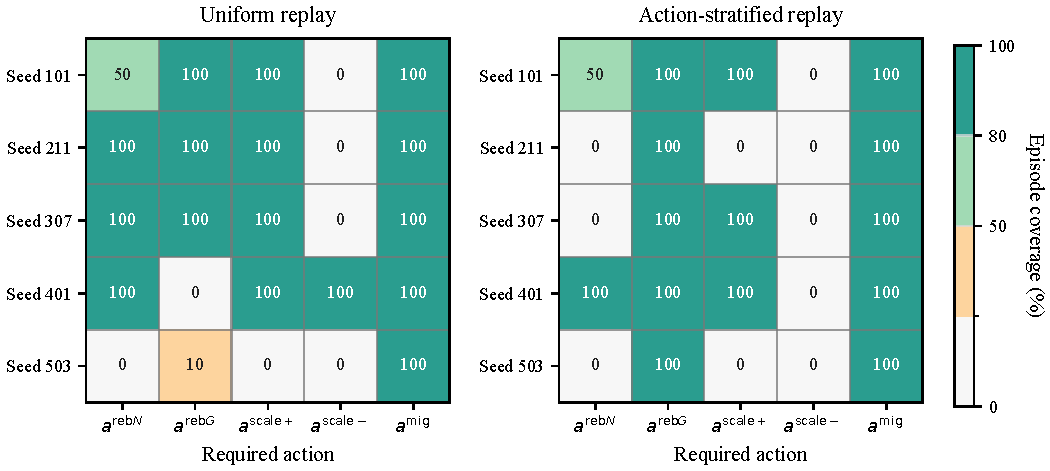
\includegraphics[width=\textwidth]{figures/v4-action-coverage.pdf}
  \caption{Fixed-validation episode coverage for required actions in the two
  v4 development runs.  A cell gives the percentage of admissible episodes in
  which the frozen candidate selected the indicated action; the predeclared
  pass threshold was $80\%$ for every column in one row.}
  \Description{Two five-by-five square heatmaps compare uniform and
  action-stratified replay.  Rows are candidate seeds and columns are the five
  required intervention actions.  A vertical color bar ranges from zero to one
  hundred percent.  No row reaches at least eighty percent in all five columns,
  primarily because scale-down remains zero.}
  \label{fig:v4-action-coverage}
\end{figure}

All ten candidates passed the scripted scenario-feasibility checks and every
fault-safety contract. No row in
Figure~\ref{fig:v4-action-coverage} passes all five policy-coverage conditions.
Uniform-replay seed 401 exercises scale-down but misses backlog rebalancing;
the other uniform candidates miss scale-down.  Every action-stratified
candidate misses scale-down, and several also miss subscription rebalancing or
scale-up. Action-stratified replay left gaps in frozen-policy action coverage.
Under the declared stopping rule, both v4 studies ended at the development
gate and retained their checkpoints for diagnosis. Their results concern
action coverage rather than new holdout performance estimates.

V5 then changed only the scale-down admissibility rule and used fresh candidate
and validation seeds. The historical target-metric checks passed, including a
$49.6\%$ connection-cost reduction for scale-down. All five frozen candidates passed every fault guard and
selected $a^{\mathrm{reb}G}$, $a^{\mathrm{scale}+}$, and
$a^{\mathrm{mig}}$ in all ten intended validation episodes.  However, each
selected $a^{\mathrm{reb}N}$ and $a^{\mathrm{scale}-}$ in zero of ten intended
episodes.  For the diagnostic candidate with the best reward, we evaluated each missed
action for one step from the same state. Both improved reward, but its Q-values ranked \emph{stay}
higher. A later audit showed that the old $a^{\mathrm{scale}+}$ action reduced
its declared maximum-subscription metric by $21.78\%$ but lowered mean scalar
reward by 0.04946 relative to static placement. The v5 diagnostics therefore
distinguish missed one-step reward gains from a scale-up implementation that
conflicted with its reward objective. The coverage gate was not met, and the
study ended without a holdout evaluation.

V6 changed only the scale-up contract. The revised $a^{\mathrm{scale}+}$ opens
one connection and performs bounded, receipt-gated $a^{\mathrm{reb}N}$ moves
until the subscription target is restored or no eligible move remains. In the
locked ten-seed preflight, the option improved mean interval reward by 0.04350
with a paired bootstrap 95\% interval of [0.03559, 0.05114]. It reduced the
mean maximum subscriptions per connection by 38.824, with interval [-38.824,
-38.824]. Every episode restored the target using exactly 50 moves, without an
executor no-op or scale-down reversal. This scripted preflight verifies the
revised action contract in the simulator; learned selection is evaluated in
the study below.

The locked v6 study then tested each combination of Target-Max or Double-DQL
bootstrapping with squared or Huber temporal-difference loss. Each arm trained five fresh
candidates for $20{,}000$ transitions and evaluated them on ten fresh
development-validation seeds. Table~\ref{tab:v6-factorial-coverage} reports
the number of candidates passing each action gate. Every candidate passed all
four safety scenarios, but no candidate passed all five action gates. The
predeclared requirement of at least four fully eligible candidates was
therefore unmet in every arm. No policy was selected and no holdout was defined
or executed. Squared and Huber loss magnitudes are not ranked against each
other because the two losses have different numerical scales.

\begin{table}[t]
  \caption{V6 development-gate results. Each action and safety entry is the
  number of passing candidates out of five. TM denotes Target-Max bootstrap;
  DDQL denotes Double-DQL. An arm required at least four candidates that each
  passed all action and safety gates.}
  \Description{Four rows report action coverage and safety counts for the v6
  Target-Max and Double-DQL arms with squared and Huber losses. Every arm has
  zero fully eligible candidates. All safety counts are five, while scale-up is
  zero except for one passing candidate in the Target-Max Huber arm.}
  \label{tab:v6-factorial-coverage}
  \centering
  \small
  \setlength{\tabcolsep}{3pt}
  \begin{tabular}{llccccccc}
    \toprule
    Arm & Learner/loss & Eligible & $a^{\mathrm{reb}N}$ & $a^{\mathrm{reb}G}$ & $a^{\mathrm{scale}+}$ & $a^{\mathrm{scale}-}$ & $a^{\mathrm{mig}}$ & Safety \\
    \midrule
    A & TM/squared & 0 & 0 & 1 & 0 & 5 & 5 & 5 \\
    B & DDQL/squared & 0 & 2 & 2 & 0 & 5 & 5 & 5 \\
    C & TM/Huber & 0 & 3 & 5 & 1 & 5 & 5 & 5 \\
    D & DDQL/Huber & 0 & 4 & 5 & 0 & 5 & 5 & 5 \\
    \bottomrule
  \end{tabular}
\end{table}

\FloatBarrier
The cap-restoring executor improves the fixed reward, while learned selection
varies across candidates. The diagnostics distinguish the corrected action
contract from policy coverage. They leave the individual effects of value
estimation, visited states, replay sampling, and credit across several moves
unresolved.

\bibliographystyle{ACM-Reference-Format}
\bibliography{example}


\end{document}
